\documentclass{article}

\usepackage{coursenotes}

\set{AuthorName}{TC Fraser}
\set{Email}{tcfraser@tcfraser.com}
\set{Website}{www.tcfraser.com}
\set{ClassName}{Electricity \& Magnetism 3}
\set{School}{University of Waterloo}
\set{CourseCode}{Phys 442}
\set{InstructorName}{Chris O'Donovan}
\set{Term}{Fall 2016}
\set{Version}{1.1 - Course Complete}

\draftprofile[TC Fraser]{TC}{Purple}

\pgfplotsset{
    standardplot/.style={
        axis x line=middle,
        axis y line=middle,
        enlarge x limits=0.05,
        enlarge y limits=0.05,
        every axis x label/.style={at={(current axis.right of origin)},anchor=north east},
        every axis y label/.style={at={(current axis.above origin)},anchor=north east},
        ytick=\empty,
        xtick=\empty,
        width=3in,
        height=2.5in,
        axis line style=thick,
    }
}
\begin{document}

\titlePage

\tableOfContents

\disclaimer

\section{Review}

\subsection{Coordinates and Symmetry}

A clever choice of coordinates systems typically makes solving a problem considerably easier. Mathematically, this is due to \textit{Noether's Theorem}. A typical three dimensional Lagrangian will have three dependent generalized coordinates $L = L \br{x,y,z} = L \br{s,\theta,\zeta} = \cdots$. However, if one can identify generalized coordinates $q$ that make the Lagrangian invariant $\pder{L}{q} = 0$, then the \textit{Euler-Lagrange} equations are considerably similar,
\[ \der{}{t}\br{\pder{L}{\dot{q}}} - \pder{L}{q} = 0 \implies \pder{L}{\dot{q}} = \textrm{const.} \implies L \propto \dot{q} \]
As such, the number of equations that remain to solved has been reduced.

\subsection{Review Problems}

\begin{center}
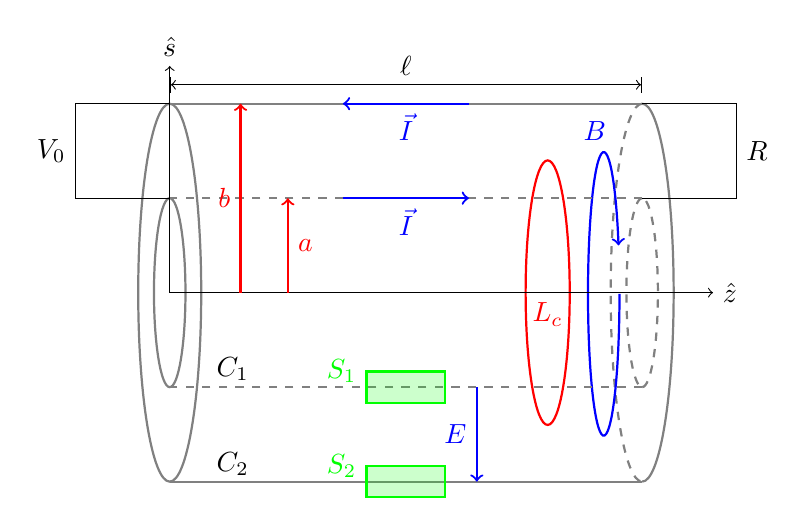
\begin{tikzpicture}[axis/.style={->,black}, conductor/.style={gray}]
    \pgfmathsetmacro\R{1.2}
    \pgfmathsetmacro\skew{0.2}
    \pgfmathsetmacro\outf{2}
    \pgfmathsetmacro\Lhalf{3}
    \pgfmathsetmacro\wire{\outf*\R - \R}

    \coordinate (top) at (\Lhalf,0);
    \coordinate (bot) at (-\Lhalf,0);
    % \coordinate (topshift) at (\R,\R);
    % \draw[thick] (top) ellipse (0.2 and 1);
    \draw[conductor, thick] (-\Lhalf,0) ellipse ({\skew} and {\R});
    \draw[conductor, thick] (-\Lhalf,0) ellipse ({\outf*\skew} and {\R*\outf});
    \draw[thick, red, ->] (0.6*\Lhalf,0) ellipse ({0.7*\outf*\skew} and {0.7*\R*\outf});
    \draw[thick, red] (0.6*\Lhalf,0) node[below]{$\s{L}_c$};
    \draw[conductor, thick, dashed] (\Lhalf,\R) arc [start angle=90, end angle=270, x radius={\skew}, y radius={\R}];
    \draw[conductor, thick, dashed] (\Lhalf,-\R) arc [start angle=-90, end angle=90, x radius={\skew}, y radius={\R}];
    \draw[conductor, thick, dashed] (\Lhalf,\R*\outf) arc [start angle=90, end angle=270, x radius={\outf*\skew}, y radius={\outf*\R}];
    \draw[conductor, thick, solid] (\Lhalf,-\R*\outf) arc [start angle=-90, end angle=90, x radius={\outf*\skew}, y radius={\outf*\R}];

    \draw[blue, thick, <-] (0.9*\Lhalf,\R-0.50*\R) arc [start angle=20, end angle=360, x radius={\skew}, y radius={1.5*\R}];
    \draw[blue, thick] (0.8*\Lhalf,1.5*\R) node[above]{$\ve B$};
    % \draw[thick] (\R, -\R) arc [start angle=-90, end angle=90, x radius=0.2, y radius=1];
    % \draw[thick, blue, <-] (0.5, -1.3) arc [start angle=-60, end angle=60, x radius=0.3, y radius=1.5];
    % \draw[thick, blue] (0.5, 1.3) node[right]{$\ve{B}$};
    % \draw[thick, dashed, red, fill, fill opacity=0.2] (0.5, 0) arc [start angle=0, end angle=360, x radius=0.2, y radius=1] node[left, fill opacity=1.0]{$\s{S}$};
    \draw[conductor,thick] (\Lhalf,\R*\outf) -- (-\Lhalf,\R*\outf);
    \draw[conductor,thick] (\Lhalf,-\R*\outf) -- (-\Lhalf,-\R*\outf);
    \draw[conductor,thick, dashed] (\Lhalf,-\R) -- (-\Lhalf,-\R);
    \draw[conductor,thick, dashed] (\Lhalf,\R) -- (-\Lhalf,\R);
    \draw[] (\Lhalf,\R) -- (\Lhalf + \wire,\R) -- node[right]{$R$} (\Lhalf + \wire,\R + \wire) -- (\Lhalf,\R + \wire);
    \draw[] (-\Lhalf,\R) -- (-\Lhalf - \wire,\R) -- node[left]{$V_0$} (-\Lhalf - \wire,\R + \wire) -- (-\Lhalf,\R + \wire);
    \draw[|<->|] (-\Lhalf,1.1*\outf*\R) -- node[above]{$\ell$} (\Lhalf,1.1*\outf*\R);

    \draw[thick, blue] (-0.8, \R) edge[->] node[below]{$\vec{I}$} (0.8, \R);
    \draw[thick, blue] (-0.8, \outf*\R) edge[<-] node[below]{$\vec{I}$} (0.8, \outf*\R);

    \draw[->, thick, blue] (0.3*\Lhalf, -\R)-- node[left]{$\ve E$}(0.3*\Lhalf, -\outf*\R) ;

    \draw[thick] (-\Lhalf+0.8, -\R-0.05) node[above]{$\s{C}_1$};
    \draw[thick] (-\Lhalf+0.8, -2*\R-0.05) node[above]{$\s{C}_2$};

    \draw[axis] (-\Lhalf, 0)--(1.3*\Lhalf, 0) node[right]{$\hat{z}$};
    \draw[->, thick, red] (-0.5*\Lhalf, 0)--node[right]{$a$} (-0.5*\Lhalf, \R) ;
    \draw[->, thick, red] (-0.7*\Lhalf, 0)-- node[left]{$b$}(-0.7*\Lhalf, \outf*\R) ;
    \draw[axis] (-\Lhalf, 0)--(-\Lhalf, 1.2*\outf*\R) node[above]{$\hat{s}$};
    \draw[thick, green, fill, fill opacity=0.2] (-0.5, -\R + 0.2) node[above, left, fill opacity=1.0]{$\s{S}_1$} -- (-0.5, -\R - 0.2) -- (0.5, -\R - 0.2) -- (0.5, -\R + 0.2) -- cycle;
    \draw[thick, green, fill, fill opacity=0.2] (-0.5, -\outf*\R + 0.2) node[above, left, fill opacity=1.0]{$\s{S}_2$} -- (-0.5, -\outf*\R - 0.2) -- (0.5, -\outf*\R - 0.2) -- (0.5, -\outf*\R + 0.2) -- cycle;

\end{tikzpicture}
\end{center}
First consider the problem of two coaxial cables. There are two key symmetries that need to be exploited. First, the entire configuration of charges and currents are left invariant under rotations about the $z$-axis. Therefore the electric field and magnetic fields \text{cannot} depend on $\phi$,
\[ \ve B\br{z, s, \phi} = \ve B\br{z, s} \qquad \ve E\br{z, s, \phi} = \ve E\br{z, s} \]
Secondly, we take the conductors to be very long $(\ell \gg 1)$ exposing translation symmetries along the $z$-axis. Therefore,
\[ \ve B\br{z, s, \phi} = \ve B\br{s} \qquad \ve E\br{z, s, \phi} = \ve E\br{s} \]
Furthermore, since the current $\ve I$ is constant, the electric field only depends on the distribution of charges $\la$. Since the global charge distribution is left invariant under inversion of the $\hat{z}$ or $\hat{\phi}$ directions, the electric field can only be radial outward\footnote{A manifestation of $\vdel \times \ve E = \ve 0$},
\[ \ve E = E\br{s} \hat{s} \eq \label{eq:2_radial}\]
Analogously, the charge distribution $\la$ is constant in time ($\pder{\la}{t} = 0$). Therefore the magnetic field only depends on global configurations of current $\ve I$. Suppose $\ve B$ had a contribution in the tangential direction ($\hat{z} \cdot \ve B > 0$). Then by inverting the $z$-axis, the sign of the currents have changed but $\ve B$ has not\footnote{As a pseudo-vector, the direction of $\vB$ needs to be inverted when acted upon by coordinate symmetries. Therefore $B_z \mapsto B_z$ whenever $z \mapsto z$}. Therefore $\hat{z} \cdot \ve B < 0$ which is a contradiction. Therefore $\ve B$ has no tangential components $\ve B \cdot \hat{z} = 0$. An analogous argument can demonstrate that the magnetic field carries no radial components $\ve B \cdot \hat{s} = 0$ (i.e. currents are flipped by inversion of the $s$-axis). However, this argument does not hold for radial components. The currents are left \textit{invariant} under $\hat{\phi}$ inversions. Therefore\footnote{A manifestation of $\vdel \cdot \ve B = 0$},
\[ \ve B = B\br{s} \hat{\phi} \eq \label{eq:2_phi}\]

Now that \cref{eq:2_radial,eq:2_phi} have been established by symmetries, it becomes trivial to discover surface boundary conditions for $\ve E$ and $\ve B$.

Let $\s{C}_1$ denote the inner conductor and $\s{C}_2$ denote the outer conductor. Parallel boundary conditions for $\ve E$ can be obtained from \cref{eq:2_radial},
\[ E_{\parallel \s{C}_1} = E_{\parallel \s{C}_2} = 0 \eq \label{eq:e_boundary_1}\]
Which can be read as: \textit{The components of $\ve E$ parallel to the conductor surfaces $\s{C}_i$ at $\s{C}_i$ are zero.} Analogously by \cref{eq:2_phi}, we have that,
\[ B_{\perp \s{C}_1} = B_{\perp \s{C}_2} = 0 \eq \label{eq:b_boundary_1} \]

Let $\di_{\ep} \s{C}_i$ denote the Gaussian surface obtained from taking the boundary of conductor $\s{C}_i$ and expanding its radius by an amount $\ep \in \R$. Next consider Maxwell's equations and the charge contained in $\di_{\ep} \s{C}_2$ and $\di_{-\ep} \s{C}_1$:
\[ \vdel \cdot \ve E = \f{\rho}{\ep_0} \implies \iint_{\s{S}} \dif \ve a \cdot \ve E = \f{q\tsb{enc}}{\ep_0} \]
Since all of the charge is allocated to the surface of the conductors, the enclosed charge for $\s{S} = \di_{-\ep} \s{C}_1$ is zero. There is also no enclosed charge for $\s{S} = \di_{\ep} \s{C}_2$ since there is a charge $\ell \la$ on $\s{C}_1$ and $-\ell \la$ on $\s{C}_2$. Therefore it must be that,
\[E_\perp\br{a^{-}} = 0 \qquad E_\perp\br{b^{+}} = 0 \eq \label{eq:e_boundary_2}\]
To obtain the perpendicular boundary conditions for $\ve{E}$ between the two conductors consider two Gaussian surfaces $\s{S}_1$ and $\s{S}_2$ (depicted) that are rectangular prisms (length $l$, angular spread $\De \phi$, height $h \ll 1$, oriented outward) that curve along with the surface of their respective conductors. Focus on $\s{S}_1$ as an example,
\[ \iint_{\s{S}_1} \dif \ve a \cdot \ve E = E_\perp\br{a^{+}}\int_{\s{S}^{+}_1} \dif a = E_\perp\br{a^{+}} \br{\De \phi a l} = \f{q\tsb{enc}}{\ep_0} = \la \cdot \br{\f{\De \phi}{2 \pi}l} \f{1}{\ep_0} \eq \label{eq:surf_arb}\]
Therefore,
\[E_\perp\br{a^{+}} = \f{\la}{2 \pi a \ep_0} \qquad E_\perp\br{b^{-}} = \f{\la}{2 \pi b \ep_0} \eq \label{eq:e_boundary_3}\]
Analogously, let $\s{L}_c$ be a Amperian loop of radius $c$ (depicted),
\[ \vdel \times \vB = \mu_0 \ve J \implies \oint_{\s{L}_c} \dif \ve l \cdot \ve B = \mu_0 I\tsb{enc}  \eq \label{eq:loop_c}\]
Since loops with radius $c < a$ or $c > b$ enclose no (net-)current, the tangential boundary conditions become,
\[ B_\parallel\br{a^{-}} = 0 \qquad B_\parallel\br{b^{+}} = 0 \eq \label{eq:b_boundary_2}\]
However when $c \to a^{+}$, $I\tsb{enc} \to I$,
\[ \oint_{\s{L}_{a^{+}}} \dif \ve l \cdot \ve B = 2 \pi a B_{\parallel}\br{a^{+}} = \mu_0 I \]
Which by analogy yields,
\[ B_\parallel\br{a^{+}} = \f{\mu_0 I }{2 \pi a} \qquad B_\parallel\br{b^{-}} = \f{\mu_0 I }{2 \pi b}  \eq \label{eq:b_boundary_3}\]
Therefore \cref{eq:e_boundary_1,eq:e_boundary_2,eq:e_boundary_3} and \cref{eq:b_boundary_1,eq:b_boundary_2,eq:b_boundary_3} define the complete set of boundary conditions for the electric and magnetic field respectively.\\

In summary, symmetries dictate that the electric field is purely radial and the magnetic field is purely azimuthal. Moreover, the electric and magnetic fields are only non-zero between the conducts $\s{C}_1$ at $a$ and $\s{C}_2$ at $b$. It is also clear that the electric field points radially outward from the central axis and the magnetic field points in the direction depicted above. \\

The boundary conditions both seem to scale as ${1}/{s}$ indicating that the relative strength of either field decreases and one moves radial outward. Geometrically, the fields between the two conductors behave precisely like the field around the inner conductor (without the presence of $\s{C}_2$) on \textit{capped} at $s > b$. The outer conductor $\s{C}_2$ shields the fields generated by $\s{C}_2$. \\

The electric potential is defined in terms of the electric field, $\ve E = - \vdel V$. Therefore a qualitative description of $\ve E$ induces a qualitative description of $V$. First, $\ve E = E\br{s} \hat{s}$ is a function of only $s$; thus $V$ can be constructed to only depend on $s$ as well.
\[ E\br{s} = - \der{}{s} V\br{s} \eq \label{eq:etov}\]
In doing do, any cylinder coaxial to cylinders $\s{C}_1$ and $\s{C}_2$ will form an equipotential surface. Additionally, since the there is a battery connecting the two coaxial cables,
\[ V\br{a} = V_0 \qquad V\br{b} = 0 \eq \label{eq:vbound} \]
This is in agreement with the idea that the electric field decreases in magnitude as one moves radially outward.\\

In order to obtain the magnetic field between the conductors, recall \cref{eq:loop_c} but instead leave $c$ arbitrary $a \leq c \leq b$:
\[ \oint_{\s{L}_c} \dif \ve l \cdot \ve B = B\br{c} \oint_{\s{L}_c} \dif l = B\br{c} 2 \pi c = \mu_0 I\tsb{enc} = \mu_0 I \]
Therefore,
\[ \ve B \br{s} = \begin{cases}
    \ve 0 & s \leq a \\
    \f{\mu_0 I}{2 \pi s}\hat{\phi} & a \leq s \leq b \\
    \ve 0 & s \geq b
\end{cases} \]
Which satisfies boundary conditions \cref{eq:b_boundary_1,eq:b_boundary_2,eq:b_boundary_3} by construction.\\

In order to obtain the electric field between the conductors, recall \cref{eq:surf_arb} and consider an arbitrary cylindrical Gaussian surface $\s{S}$ with radius $c$ such that $a \leq c \leq b$ and length $\ell$,
\[ \iint_{\s{S}} \dif \ve a \cdot \ve E = E\br{c} \iint_{\s{S}} \dif a = E\br{c} 2 \pi c \ell = \f{q\tsb{enc}}{\ep_0} = \f{1}{\ep_0} \ell \la  \]

Therefore,
\[ \ve E \br{s} = \begin{cases}
    \ve 0 & s \leq a \\
    \f{\la}{2 \pi s \ep_0}\hat{s} & a \leq s \leq b \\
    \ve 0 & s \geq b
\end{cases} \]
Which satisfies boundary conditions \cref{eq:e_boundary_1,eq:e_boundary_2,eq:e_boundary_3} by construction. In order to eliminate $\la$ we can make use of \cref{eq:etov} and \cref{eq:vbound}. Letting $s$ run from $a$ to $b$ be an arbitrary radius to be determined,
\[ \De V = 0 - V_0 = -\intl_{a}^{b} \dif s' E\br{s'} = -\intl_{a}^{b} \dif s' \f{\la}{2 \pi s \ep_0} = -\f{\la}{2 \pi \ep_0} \ln\br{\f{b}{a}} \]
Therefore,
\[ \la = 2 \pi \ep_0 V_0 \br{\ln\br{\f{b}{a}}}^{-1} \]
Rewriting the electric field,

\[ \ve E \br{s} = \begin{cases}
    \ve 0 & s \leq a \\
    \f{V_0}{s} \br{\ln\br{\f{b}{a}}}^{-1}\hat{s} & a \leq s \leq b \\
    \ve 0 & s \geq b \eq \label{eq:e_field_2}
\end{cases} \]
Inside the conductor, there are no sources of charge. Consequently,
\[ \del^2 V = 0 \]
In cylindrical coordinates,
\[ \f{1}{s}\pder{}{s}\br{s \pder{V}{s}} + \f{1}{s^2} \pdder{V}{\phi} + \pdder{V}{z} = 0 \]
But by symmetry, $V$ has no dependence on $\phi$ or $z$ and thus,
\[ \der{}{s}\br{s \der{V}{s}} = 0 \]
Therefore let $k_1$ be some constant,
\[ s \der{V}{s} = k_1 \]
\[ \der{V}{s} = \f{k_1}{s} \]
At this point, one can compare $\f{k_1}{s}$ with $E\br{s}$ directly. Nonetheless,
\[ V\br{s} = k_1 \ln \br{s} + k_2 \]
Matching boundary conditions given by \cref{eq:vbound},
\[ V\br{b} = 0 = k_1 \ln \br{b} + k_2 \]
\[ V\br{a} = V_0 = k_1 \ln \br{a} + k_2 \]
Therefore,
\[ V_0 = k_1 \ln \br{a} + k_2 = k_1 \ln \br{a} - k_1 \ln \br{b} = k_1 \ln \br{\f{a}{b}} \]
And thus,
\[ k_1 = \f{V_0}{\ln \br{\f{a}{b}}} \qquad k_2 = - \f{V_0 \ln \br{b}}{\ln \br{\f{a}{b}}}  \]
Therefore the potential is given by,
\[ V\br{s} = V_0\f{\ln\br{\f{s}{b}}}{\ln \br{\f{a}{b}}} \eq \label{eq:Vlapl}\]
Using \cref{eq:Vlapl} and \cref{eq:etov},
\[ E\br{s} = - \der{}{s} \br{V_0\f{\ln\br{\f{s}{b}}}{\ln \br{\f{a}{b}}}} = -\f{V_0}{s}\br{\ln\br{\f{a}{b}}}^{-1}\]
Matching \cref{eq:e_field_2} exactly.

\newcommand{\coord}[4]{\coordinate (#1) at (#2,#3,#4);}
\newcommand{\cylindcoord}[4]{\coordinate (#1) at ({#2*cos(#3)},{#2*sin(#3)},{#4});}
\newcommand{\spherecoord}[4]{\coordinate (#1) at ({#2*cos(#3)*sin(#4)},{#2*sin(#3)*sin(#4)},{#2*cos(#4)});}

%polar coordinates of visibility
\pgfmathsetmacro\th{70}
\pgfmathsetmacro\az{110}
\tdplotsetmaincoords{\th}{\az}

\begin{center}

\begin{tikzpicture} [scale=1, tdplot_main_coords, axis/.style={->,black}]

    %parameters of the cone
    \pgfmathsetmacro\R{1.6} % Radius of cylinder
    \pgfmathsetmacro\H{3} % Height of cylinder
    \pgfmathsetmacro\aL{3.5} % Length of the axis

    \pgfmathsetmacro\rr{4}
    \pgfmathsetmacro\r{4}
    \pgfmathsetmacro\rphi{60}
    \pgfmathsetmacro\rh{4}
    \cylindcoord{r}{\rr}{\rphi}{\rh}
    \cylindcoord{rflat}{\rr}{\rphi}{0}
    \cylindcoord{rp}{\R}{-40}{1.4}
    \cylindcoord{radius}{\R}{-60}{0}
    \cylindcoord{hmark}{1.8}{-70}{0}
    \cylindcoord{hmarktop}{1.8}{-70}{\H}

    % Axis declaration
    \coordinate (O) at (0,0,0);
    \coordinate (x) at (1,0,0);
    \coordinate (y) at (0,1,0);
    \coordinate (z) at (0,0,1);
    \coordinate (X) at ($\aL*(x)$);
    \coordinate (Y) at ($\aL*(y)$);
    \coordinate (Z) at ($\aL*(z)$);

    %draw axes
    \draw[axis] (O)--(X) node[anchor=north]{$\hat{x}$};
    \draw[axis] (O)--(Y) node[anchor=north]{$\hat{y}$};
    \draw[axis] (O)--(Z) node[anchor=south]{$\hat{z}$};

    % % angles for transformed lines
    \pgfmathsetmacro\PhiOne{180+(\az)}
    \pgfmathsetmacro\PhiTwo{0+(\az)}

    % % coordinates for transformed surface lines
    \pgfmathsetmacro\sinPhiOne{{sin(\PhiOne)}}
    \pgfmathsetmacro\cosPhiOne{{cos(\PhiOne)}}
    \pgfmathsetmacro\sinPhiTwo{{sin(\PhiTwo)}}
    \pgfmathsetmacro\cosPhiTwo{{cos(\PhiTwo)}}

    % % draw basis circle
    \tdplotdrawarc[tdplot_main_coords]{(O)}{\R}{\PhiOne}{360+\PhiTwo}{}{}
    \tdplotdrawarc[tdplot_main_coords]{(O)++($\H*(z)$)}{\R}{0}{360}{}{}
    \tdplotdrawarc[tdplot_main_coords,dashed]{(O)}{\R}{\PhiTwo}{\PhiOne}{}{}

    \tdplotdrawarc[tdplot_main_coords,color=red]{(O)}{0.3}{0}{\rphi}{anchor=north}{$\phi$}

    % % displaying tranformed surface of the cone (rotated)
    \draw (\R*\cosPhiOne,\R*\sinPhiOne,\H) -- (\R*\cosPhiOne,\R*\sinPhiOne,0);
    \draw (\R*\cosPhiTwo,\R*\sinPhiTwo,\H) -- (\R*\cosPhiTwo,\R*\sinPhiTwo,0);

    \draw[thick,color=red, ->] (O) -- node[midway, below]{$\vr$} (r);
    \draw[thick,color=blue, ->] (O) -- node[midway, below]{$\vr'$} (rp);
    \draw[thick, ->] (rp) -- node[midway, below]{$\vec{\rcurs}$} (r);
    \draw[dashed,color=red, ->] (O) -- node[midway, below left]{$s\hat{s}$} (rflat);
    \draw[dashed,color=red, ->] (rflat) -- node[midway, right]{$\zeta\hat{\zeta}$} (r);
    \draw[->] (O) -- node[midway, below]{$R$} (radius);
    \draw[|<->|] (hmark) -- node[midway, left]{$h$} (hmarktop);

\end{tikzpicture}
\end{center}

\textbf{A1.1}: Use cylindrical coordinates with $\zeta$ along the axis of the cable,

\[ V\br{\zeta} = \f{1}{4 \pi \ep_0} \int_{\s{C}}\f{\dif \rho}{\rcurs} \]

Where $\ve{\rcurs} = \ve{r} - \ve{r}'$, $\ve{r}'$ is the source point and $\ve{r}$ is the field point. The entire cylinder is the set of all source points $\ve{r}'$ that are contained inside $\abs{\ve{r}'} \leq R$.
\[ \ve{r} = \zeta \hat{\zeta} \]
\[ \ve{r}' = s' \hat{s}' + \zeta' \hat{\zeta} \]

\[ V\br{\zeta} = \f{\rho}{4 \pi \ep_0} \int_{\s{C}}\f{\dif V}{\abs{\ve{r} - \ve{r}'}} \]

Where $ \dif V = s \dif s \dif \theta \dif \zeta$. One can then find the electric \textit{field} by doing $\ve{E} = - \vdel V = E_{\zeta} \hat{\zeta} = -\pder{V}{\zeta} \hat{\zeta}$

\textbf{A1.2}:

Between the two conductors, there will be a radial electric field $\ve{E} = E\br{s} \hat{s}$ and parallel magnetic field $\ve{B} = B\br{s} \hat{\zeta} $. Outside the two conductors, there will be no electric or magnetic field.

\[ E^{\parallel}\tsb{vac} = 0 \]
\[ E^{\perp}\tsb{vac} = \f{\si}{\ep_0} \]
\[ \vdel \cdot \ve{E} = \f{\rho}{\ep_0} \]

For part g), use Laplace's equation $\del^2 V = 0$. In cylindrical coordinates, Laplace's equation is,
\[ \del^2 V = \f{1}{s} \pder{}{s}\br{s \pder{V}{s}} = 0 \]
Cylindrical coordinates gives us the following symmetries $\pder{V}{\phi} = \pder{V}{\zeta} = 0$.
Solving this system gives the potential in terms of $s$: $V\br{s} = \cdots$. Then the electric field can then be obtained via $\vec{E} = - \vdel V$.

\textbf{A1.3}: Using cylindrical coordinates once again, the electric field is going to be radial outwards to the uniform charge density. For the uniform density cylinder, construct a Gaussian surface cylindrically around the cylinder. For the current density cylinder, the current density is the current per cross sectional area. Construct an Amperian loop,
\[ \oint_{\s{A}} \dif \vec{\ell} \cdot \vec{B} = \mu I\tsb{enc}  \]
Part e), finding the vector potential,
\[ A\br{\vr} = \f{\mu_0}{4\pi} \int_{\s{C}} \dif \tau' \f{\vec{J}\br{\vec{r}}}{\rcurs} \]
Evidently, $\hat{s}$ and $\hat{s}'$ are in \textit{different} directions.
Solving such an equation yields,
\[ A\br{s} = \f{\mu_0}{4 \pi} \int_{0}^{2\pi} \dif \phi' \int_{0}^{a} s' \dif s' \int_{-\inf}^{\inf} \dif \zeta' \f{J\br{s}}{\abs{s \hat{s} - s' \hat{s}' - \zeta' \hat\zeta}} \]
Recognize the structure of the potential integral,
\[ V\br{s} = \f{1}{4\pi \ep_0} \int_{\s{C}} \dif \tau' \f{\rho\br{r'}}{\rcurs} = \f{\rho_0}{4 \pi \ep_0} \int_{\s{C}} \f{\dif \tau'}{\rcurs}\]
Comparing to the vector potential, we have an equivalent integral (up to a constant).
\[ A\br{s} = \f{\mu_0 J_0}{4 \pi} \int_{\s{C}} \f{\dif \tau'}{\rcurs} \]
For question f), use the definition of $\vec{B}$ in terms of $\vec{A}$,
\[ \vec{B} = \vdel \times \vec{A} \]
Further, recall that if $\vec{E} = -\vdel V$, then by Stoke's theorem for some loop $\s{L}$,
\[ V = - \int_{\s{L}} \dif \vec{\ell} \cdot \vec{E} \]

\subsection{Conservation Laws}
Beginning with one of Maxwell's equations,
\[ \vdel \times \vec{B} = \mu_0 \vec{J} + \mu_0 \ep_0 \pder{\vec{E}}{t} \]
Taking the divergence of the above equation,
\[ \cancelto{0}{\vdel \cdot \br{\vdel \times \vec{B}}} = \mu_0 \vdel \cdot \vec{J} + \mu_0 \ep_0 \pder{}{t}\br{\vdel \cdot \vec{E}} \]
Luckily, the divergence of a curl is always $0$. Dividing by relevant constants we obtain the following conservation law,
\[ 0 = \vdel \cdot \vec{J} + \pder{\rho}{t} \eq \label{eq:conservation_charge}\]
This is a conservation of charge. It is a \textit{local} conservation law because it holds for all points in space $\vec{r}$. Intuitively, it claims that the rate of change of charge at a point is equal to the amount of current following in or out of the take point. \\

\textbf{A2.1}: Again using cylindrical coordinates $\vec{r} = s \hat{s} + \zeta \hat{\zeta}$. Let the current flow in such a way that the magnetic field points along the $\zeta$-axis. Let $\s{L}$ be an Amperian loop with one side at distance $\abs{\vec{r}} \to \inf$,
\[ \int_{\s{L}} \dif \vec{\ell} \cdot \vec{B} = \mu_0 I\tsb{enc} \]
The same equation can be reused to calculate the vector potential for a Gaussian surface $\s{S}$,
\[ \int_{\s{L}} \dif \vec{\ell} \cdot \vec{A} = \int_{\s{S}} \dif \vec{a} \cdot \vec{B} = \Phi \]
Where $\Phi$ is the magnetic flux through $\s{S}$. Furthermore, the energy required to set up a magnetic field is,
\[ W = \f{1}{2 \mu_0} \int_{\s{C}} \dif \tau B^2 = \f{1}{2} \int_{\s{C}} \dif \tau \vec{J} \cdot \vec{A} = \f{1}{2} L I^2 \]
Where $L$ is the self-inductance of the solenoid.

\subsection{Poynting's Theorem}
First we begin with two of Maxwell's equations,
\[ \vdel \times \vec{E} = - \pder{\ve B}{t} \eq \label{eq:poyn_max_1}\]
\[ \vdel \times \vec{B} = \mu_0 \vec{J} + \mu_0 \ep_0 \pder{\vec{E}}{t} \eq \label{eq:poyn_max_2}\]
Computing the inner product between \cref{eq:poyn_max_1} and $\vec{B}$, and the inner product between \cref{eq:poyn_max_2} and $\vec{E}$ and taking a difference,
\[ \vec{B} \cdot \br{\vdel \times \vec{E}} - \vec{E} \cdot \br{\vdel \times \vec{B}} = - \pder{}{t}\br{\f{\ep_0}{2} E^2 + \f{1}{2 \mu_0} B^2} = \mu_0 \vec{E} \cdot \vec{J}\]
Letting $\f{\ep_0}{2} E^2 + \f{1}{2 \mu_0} B^2$ be the \textbf{electromagnetic energy density} $u$, we have the following identity,
\[ \vdel\cdot\br{\vec{E} \times \vec{B}} = - \mu_0 \pder{u}{t} - \mu_0 \vec{E} \cdot \vec{J} \eq \label{eq:poyn_conservation_energy} \]
Physically \cref{eq:poyn_conservation_energy} corresponds to a conservation of energy. We refer to the term $\f{1}{\mu_0} \br{\vec{E} \times \vec{B}}$ as the Poynting vector $\vec{S}$ as it determines the direction of electromagnetic radiation. The Poynting vector $\vec{S}$ represents the power density.
\[ \vdel \cdot \vec{S} + \pder{u}{t} + \vec{E} \cdot \vec{J} = 0 \eq \label{eq:poyn_eq}\]
Much like \cref{eq:conservation_charge}, \cref{eq:poyn_eq} is a local conservation of \textit{energy}. The only algebraic difference is the term $\vec{E} \cdot \vec{J}$. If there is a flowing charge $\vec{J}$ through an electric field $\vec{E}$, then there is work done on the charge. By Gauss's theorem, the energy leaving through a surface $\s{S}$ per unit time is,
\[ \int_{\s{V}} \vdel \cdot \vec{S} \dif \tau =  \oint_{\s{S}} \dif \vec{a}\cdot \vec{S} \]
and the E-M energy in the volume $\s{V}$ is given by,
\[ \int_{\s{V}} \dif \tau u \]
Where again, $u$ is the electromagnetic energy density. If we integrate over \cref{eq:poyn_eq},
\[\int_{\s{V}} \dif \tau \br{\vdel \cdot \vec{S} +\pder{u}{t} + \vec{E} \cdot \vec{J}} = \oint_{\s{S}} \dif \vec{a}\cdot \vec{S} + \int_{\s{V}} \dif \tau \pder{u}{t} + \int_{\s{V}} \dif \tau \vec{E} \cdot \vec{J} \]
Each term in \cref{eq:poyn_eq} has it's purpose illuminated. The final term $\int_{\s{V}} \dif \tau \vec{E} \cdot \vec{J}$ corresponds to the work done on moving charges $\vec{J}$ in the volume $\s{V}$. In it important to note that there are no terms that corresponding to ``magnetic work''. \\

Consider the work done to move a charge $q$ a displacement $\dif \vec{\ell}$ by E-M forces,
\begin{align*}
\dif W &= \dif \vec{\ell} \cdot \vec{F} \\
&= \dif \vec{\ell} \cdot q \br{\vec{E} + \vec{v} \times \vec{B}}\\
&= \vec{v} \dif t \cdot q \br{\vec{E} + \vec{v} \times \vec{B}}\\
&= q \dif t \br{\vec{v} \cdot \vec{E}} + q \dif t \underbrace{\br{\vec{v} \cdot \bc{\vec{v} \times \vec{B}}}}_{= 0} \\
&= q \dif t \br{\vec{v} \cdot \vec{E}}
\end{align*}
So for a continuous charge distribution we have that $\dif q = \rho \dif \tau$ and $\rho \vec{v} = \vec{J}$. Which means that the rate of work done on the charge $\rho$ in the volume $\s{V}$ (i.e. creating the current density $\vec{J}$) is,
\[ \dot{W} = \int_{\s{V}} \dif \tau \vec{E} \cdot \vec{J} \]
We can interpret this as the work done per unit time rearranging the charge in $\s{V}$. One again \cref{eq:poyn_eq} is given by
\[ \vdel \cdot \vec{S} + \pder{u}{t} + \vec{E} \cdot \vec{J} = 0 \]
With the following interpretations,
\begin{itemize}
    \item $\vdel \cdot \vec{S}$: amount of radiation energy leaving the point $\vr$
    \item $\pder{u}{t}$: increase in E-M energy at the point $\vr$
    \item $\vec{E} \cdot \vec{J}$: the amount of work done on charges at the point $\vr$
\end{itemize}

% \begin{tikzpicture}
%     \draw[thin, dashed] (0,0) circle (2);
%     \draw[fill] (0,0) circle (0.1);
% \end{tikzpicture}

As an illustrative example, consider a parallel plate capacitor with an electric field $\vec{E}$ between them.
\begin{center}
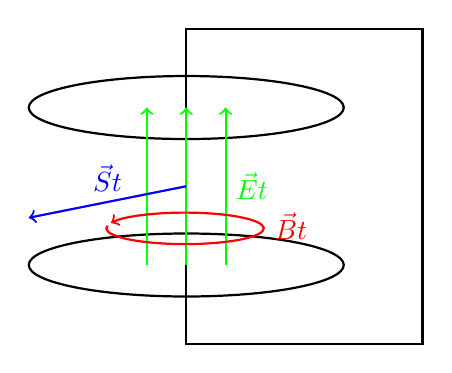
\begin{tikzpicture}
    \coordinate (top) at (0,1);
    \coordinate (bot) at (0,-1);
    \draw[thick] (top) ellipse (2 and 0.4);
    \draw[thick] (bot) ellipse (2 and 0.4);
    \draw[thick] (top) -- (0, 2) -- (3, 2) -- (3, -2) -- (0, -2) -- (bot);
    \draw[thick, green] (top) edge[<-] (bot);
    \draw[thick, green] (0.5, 1) edge[<-] node[midway, right]{$\vec{E}\br{t}$} (0.5, -1);
    \draw[thick, green] (-0.5, 1) edge[<-] (-0.5, -1);
    \draw[thick, blue] (0, 0) edge[->] node[midway, above]{$\vec{S}\br{t}$} (-2, -0.4);
    \draw[->, thick, red] (-1,-0.5) arc [start angle=-190, end angle=160, x radius=1, y radius=0.2];
    \draw[red] (1, -0.5) node[right]{$\vec{B}\br{t}$};
\end{tikzpicture}
\end{center}
We have that the magnetic field points in the $\hat{\phi}$ direction, $\vec{B} = V \hat{\phi}$. The electric field $\vec{E} = E \hat{\zeta}$, and Poynting vector are $\vec{S} = S \hat{s}$. We have that the radiation through the surface $\s{S}$,
\[ \int_{\s{S}} \dif \vec{a} \cdot \vec{S} = - \br{2 \pi a h} S \]
Therefore $\pder{U}{t} = - \br{2 \pi a h} S$ corresponding to the amount of energy flowing out of the capacitor and therefore,
\[ U = \intl_{0}^{\inf} \dif t \br{- 2 \pi a h S} = \f12 C V^2 \]

\textbf{Ex 8.1}:
\begin{center}
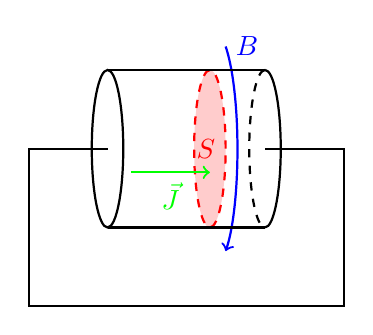
\begin{tikzpicture}
    \pgfmathsetmacro\R{1} % Radius of cylinder
    \coordinate (top) at (\R,0);
    \coordinate (bot) at (-\R,0);
    \coordinate (topshift) at (\R,\R);
    % \draw[thick] (top) ellipse (0.2 and 1);
    \draw[thick] (bot) ellipse (0.2 and 1);
    \draw[thick, dashed] (\R, \R) arc [start angle=90, end angle=270, x radius=0.2, y radius=1];
    \draw[thick] (\R, -\R) arc [start angle=-90, end angle=90, x radius=0.2, y radius=1];
    \draw[thick, blue, <-] (0.5, -1.3) arc [start angle=-60, end angle=60, x radius=0.3, y radius=1.5];
    \draw[thick, blue] (0.5, 1.3) node[right]{$\ve{B}$};
    \draw[thick, dashed, red, fill, fill opacity=0.2] (0.5, 0) arc [start angle=0, end angle=360, x radius=0.2, y radius=1] node[left, fill opacity=1.0]{$\s{S}$};
    \draw[thick] (\R, \R) -- (-\R, \R);
    \draw[thick] (\R, -\R) -- (-\R, -\R);
    \draw[thick] (top) -- (2, 0) -- (2, -2) -- (-2, -2) -- (-2, 0) -- (bot);

    \draw[thick, green] (-0.7, -0.3) edge[->] node[below]{$\vec{J}$} (0.3, -0.3);
\end{tikzpicture}
\end{center}
Inside the conductor the electric field moves parallel to its axis $\vec{E} = \f{V_0}{\ell} \hat{\zeta}$. The magnetic field is then given by,
\[ \vdel \times \vec{B} = \mu_0 \ep_0 \pder{E}{t} + \mu_0 \vec{J} \]
Integration over the surface $\s{S}$,
\[ \int_{\s{S}} \dif \vec{a} \cdot \br{\vdel \times \vec{B}} = \mu_0 \int_{\s{S}} \dif \vec{a} \cdot \vec{J} = \mu_0 I\tsb{enc} \]
Therefore computing this integral $\int \dif \vec{\ell} \cdot \vec{B}$ yields,
\[ \vec{B} = \f{\mu_0I}{2\pi a}\hat{\phi} \]
Moreover, the Poynting vector is given by,
\begin{align*}
\vec{S} &= \f{1}{\mu_0} \vec{E}\times \vec{B} \\
&= \f{1}{\mu_0} \f{V_0}{\ell} \hat{\zeta} \times \f{\mu_0 I}{2 \pi a} \hat{\phi} \\
&= -\f{V_0 I}{2\pi a \ell}\hat{s}
\end{align*}
Therefore the radiation flux,
\[ \int_{\s{S}} \dif \vec{a} \cdot \vec{S} = -\f{V_0 I}{2 \pi a \ell} \int_{\s{S}} \dif a = - V_0 I \]
Which is exactly the amount of Joule heating for a current $I$ though a wire with voltage $V_0$ across it. Using $V = I R$,
\[ \int_{\s{S}} \dif \vec{a} \cdot \vec{S} = -I^2 R \]
\textbf{Ex 8.2 (Griffiths Problem 8.13):}
A long thin solenoid of radius $a$ has a time dependent current $I_{s}\br{t}$ flowing around it. Encircling the solenoid is a ring of radius $b$ with current $I_{r}\br{t}$ ($b \gg a$) passing through it. The ring has resistance $R$. There is an induced electro-motive-force in the ring due to the solenoid,
\[ \s{E} = - \dot{\Phi}_S = - \pder{}{t}\br{\pi a^2 B_S} \]
Where $B_s = \mu_0 n I_s$. The EMF $\s{E}$ must also equal $\s{E} = I_r R$. Therefore,
\[ I_r = - \f{1}{R}\br{\mu_0 \pi a^2 n}\dot{I}_S \]
In order to calculate the electric and magnetic fields just outside solenoid, recognize that $\ve B_s = B_s\br{t} \hat{z}$ point along the axis of the solenoid. Similarly recognize that $\ve E = E \hat{\phi}$. Therefore the Poynting vector is given by,
\[ \ve S = \f{1}{\mu_0} \ve E \times \ve B_s = \f{1}{\mu_0} E B_{s} \hat{s} = ? \]
We first need to calculate $\ve E$ and $\ve B_s$. The magnetic field is known to be $\ve B = \mu_0 n I_s \hat{z}$ on axis and $\vdel \times \ve E = - \pder{\ve B}{t}$,
\[ \int \dif \ve a \cdot \vdel \times \ve E = - \der{}{t} \int \dif \ve a \cdot \ve B \]
\[ \int \dif \ve \ell \cdot \ve E = - \dot \Phi = 2 \pi a E \]
Which gives,
\[ \ve E = \f{\dot \Phi}{2\pi a}\hat{\phi} \]
The magnetic field off axis and outside the solenoid due to the ring is given by,
\[ \dif \ve B_r \br{s} = \f{\mu_0 I}{4 \pi} \f{\dif \ve \ell \times \ve \rcurs}{\rcurs^2} \]
Where $\ve \rcurs = \ve r - \ve r'$ and we take $\ve r ' = b \hat s '$ and $\ve r = z \hat z$.
\[ \ve \rcurs = z \hat z - b \hat s' \]
We will take the infinitesimal loop to be $\dif \ve \ell = b\dif \phi'\hat \phi'$.
\begin{align*}
\dif \ve \ell \times \ve \rcurs &= \br{b \hat \phi' \dif \hat \phi'}\times\br{z\hat z - b \hat s '} \\
&= a z \dif \phi' \hat s' + b^2 \dif \phi' \hat z
\end{align*}
We integrating around the loop $\s{L}$, all of the contributions in the $\hat{s}'$ directions will cancel out.
\[ \int_{\s{L}} \dif \ve \ell \times \ve \rcurs = \cdots \]
Thus,
\begin{align*}
\ve B_r &= \f{\mu_0 I_r}{4\pi} \int \f{b^2 \dif \phi' \hat z}{\br{z^2 + b^2}^{3/2}} \\
&= \f{\mu_0 I_r b^2 2 \pi \hat z}{4\pi \br{z^2 + b^2}^{3/2}} \\
&= \f{\mu_0 b^2}{2\br{z^2 + b^2}^{3/2}}I_r\hat z
\end{align*}
Therefore the Poynting vector points radial outward,
\begin{align*}
\ve S &= \f{1}{\mu_0}\ve E_r \times \ve B_r \\
&= \f{1}{\mu_0}\br{\f{\pi a^2 \mu_0 n \dot I_s}{2 \pi a} \hat \phi} \times \br{\f{\mu_0 b^2}{2\br{z^2 + b^2}^{3/2}}I_r\hat z} \\
&= \f{\mu_0}{4} a n \dot I_s \f{b^2}{\br{z^2 + b^2}^{3/2}} I_r \hat{s}
\end{align*}
Now that the Poynting vector is known, one can calculate the power radiated from the system.
\begin{align*}
P &= \int \dif \ve a \cdot \ve S \\
&= \f{\mu_0}{4} a n \dot I_s I_r b^2 \int \dif z a \dif \phi \hat s \cdot \f{1}{\br{z^2 + b^2}^{3/2}} \hat{s} \\
&= \f{\mu_0}{4} a n \dot I_s I_r b^2 \br{2 \pi a} \int \dif z \f{1}{\br{z^2 + b^2}^{3/2}} \\
&= \f{\mu_0}{4} a n \dot I_s I_r b^2 \br{2 \pi a} \f{2}{b^2} \note{Integral Table} \\
&= \mu_0 \pi a^2 n \dot I_s I_r
\end{align*}
But we know that $\mu_0 \pi a^2 n \dot I_s = - I_r R$. Therefore $P = - I_r^2 R$ as expected.\\
\textbf{A2.2:}\\
a,b) Answers in Griffiths. \\
c) Consider parallel metal strips with height $h$ and width $w$ where $h \ll w$. A current flows down one plate and up the other. The system will act as a capacitor. The magnetic field outside will be zero and non-negative inside. \\
d) Griffiths 8.1 \\
\textbf{A2.3:}\\
Positive and negative charge build up on the surfaces between the capacitor. Of course, there will be a time varying current $I\br{t}$, electric field $\ve E \br{t}$ and magnetic field $\ve B \br{t}$.

\subsection{Stress Energy Tensor}

Last week we looked at conservation laws and we found,
\[ \vdel \cdot \ve J + \pder{\rho}{t} = 0 \note{(charge)} \]
and,
\[ \vdel \cdot \ve S + \pder{u}{t} + \ve J \cdot \ve E = 0 \note{(energy)} \]
This week we will continue with momentum and angular momentum and then we will examine the Maxwell stress tensor; the field equivalent for force in Newton's second law. But first we will look at momentum.
\subsection{Momentum}
Consider two charges $+q_1$ and $-q_2$ with velocities $\ve v_1$ and $\ve v_2$. The electric field at point $2$ due to charge $1$ will be denoted $\ve E_1$. Analogously for $\ve B_1$. The net force acting on charge $q_2$ is then,
\[ \ve F_{2;E} = q_2 \ve E_1 \qquad \ve F_{2;B} = q_2 \ve v_2 \times \ve B_1 \]
\[ \ve F_{1;E} = q_1 \ve E_2 \qquad \ve F_{1;B} = q_1 \ve v_1 \times \ve B_2 \]
One will notice that $\ve F_{1;B}$ and $\ve F_{2;B}$ are not equal and opposite forces like $\ve F_{1;E}$ and $\ve F_{2;E}$ are. What does this say about Newton's third law?
\[ \sum \dve p_i = \sum \ve F\tsb{net} \]
We forgot about the fact that the electric and magnetic fields carry not only energy (via $\ve S$) but momentum as well. Recall that for photons,
\[ E = h f = \hbar \w  \]
\[ p = \f{h}{\la} = \hbar k \]
Therefore we have that,
\[ E = pc \]
Therefore knowing the energy density of the field gives you then momentum density of the field. The momentum density will be denoted $\ve g$.
\[ \ve g = \f{1}{c^2} \ve S = \mu_0 \ep_0 \ve S = \f{1}{4 \pi c} \ve E \times \ve B \]
Let $\ve f = \De \ve F / \De \tau$ be the force per \textit{unit volume} acting on a particle. The Lorentz force determines the $\ve f$.
\[ \ve f = \rho \ve E + \ve J \times \ve B\]
We can eliminate the dependence on the source terms $\rho$ and $\ve J$ by invoking Maxwell's equations,
\[ \ve f = \ep_0 \br{\vdel \cdot \ve E} \ve E + \br{\f{1}{\mu_0} \vdel \times \ve B - \ep_0 \pder{\ve E}{t}} \times \ve B \]
By product rule,
\[ \pder{}{t}\br{\ve E \times \ve B} = \ve E \times \pder{\ve B}{t} + \pder{\ve E}{t} \times \ve B \]
Invoke Maxwell's equation again $\vdel \times \ve E = - \pder{\ve B}{t}$,
\[ \pder{}{t}\br{\ve E \times \ve B} = -\ve E \times \br{\vdel \times \ve E} + \pder{\ve E}{t} \times \ve B \]
Therefore,
\begin{align*}
\ve f
&= \ep_0 \br{\vdel \cdot \ve E} \ve E + \f{1}{\mu_0} \br{\vdel \times \ve B} \times \ve B - \ep_0 \pder{\ve E}{t}\times\ve B  \\
&= \ep_0 \br{\vdel \cdot \ve E} \ve E + \f{1}{\mu_0} \br{\vdel \times \ve B} \times \ve B - \ep_0 \pder{}{t}\br{\ve E \times \ve B} - \ep_0\ve E \times \br{\vdel \times \ve E}
\end{align*}
Recognize the Poynting vector $\mu_0 \ve S = \ve E \times \ve B$. We will also make use of the product rule for the gradient,
\[ \vdel E^2 = 2 \br{\ve E \cdot \vdel} \ve E + 2 \ve E \times \br{\vdel \times \ve E} \]
After some algebra we arrive at,
\[ \ve f = \ep_0 \bs{\br{\vdel \cdot \ve E} \ve E + \br{\ve E \cdot \vdel} \ve E} + \f{1}{\mu_0} \bs{\br{\vdel \cdot \ve B} \ve B + \br{\ve B \cdot \vdel} \ve B} - \vdel \br{\f{\ep_0}{2} E^2 + \f{1}{2 \mu_0} B^2} - \mu_0 \ep_0 \pder{\ve S}{t} \eq \label{eq:messy}\]
We now introduce \term{Maxwell's stress-energy tensor} $T$ with components,
\[ T_{ij} = \ep_0 \br{E_i E_j - \f{1}{2} \de_{ij} E^2} + \f{1}{\mu_0} \br{B_i B_j - \f{1}{2} \de_{ij} B^2} \eq \label{eq:components_of_MST}\]
Where $\ve E = \sum_{i} E_i \hat{e}_i$ and $\ve B = \sum_{i} B_i \hat{e}_i$. We now have that \cref{eq:messy} gives,
\[ \ve f = \vdel \cdot T - \ep_0 \mu_0 \pder{\ve S}{t} \]
Where the divergence of $T$ can be written as,
\[ \pder{T_{ij}}{x_i} = \ep_0 \br{\pder{E_i}{x_i} E_j + E_i \pder{E_j}{x_i} - \f12 \pder{E^2}{x_j}} + \f{1}{\mu_0} \br{\pder{B_i}{x_i} B_j + B_i \pder{B_j}{x_i} - \f12 \pder{B^2}{x_j}} \]
As defined $\ve F = \int_{\s{V}} \dif \tau \ve f$ is the net mechanical force acting on the matter in a volume $\s{V}$. Therefore,
\begin{align*}
\der{}{t} \ve p\tsb{mech} &= \int_{\s{V}} \dif \tau \ve f \\
&= \int_{\s{V}} \dif \tau \br{\vdel \cdot T - \ep_0 \mu_0 \pder{S}{t}} \\
&= \oint_{\s{S}} \dif \ve a \cdot T - \der{}{t} \int_{\s{V}} \dif \tau \ep_0 \mu_0 \ve S
\end{align*}
We usually define the second term here to be the momentum contained in the electromagnetic field,
\[ \ve p\tsb{em} = \int_{\s{V}} \dif \tau \ep_0 \mu_0 \ve S \]
Therefore the conservation of momentum is,
\[ \der{}{t} \br{\ve p\tsb{mech} + \ve p\tsb{em}} = \oint_{\s{S}} \dif \ve a \cdot T \eq \label{eq:conservation_momentum}\]

To draw intuition from continuum mechanics, the \term{Cauchy stress tensor} is a representation of the total forces acting on a chunk $\s{V}$ of a material due to the neighboring pieces $\s{N}\br{\s{V}}$. Each neighboring chunk $n \br{\s{V}}$ can exert parallel or shear forces on $\s{V}$. This defines a matrix on force components on each face of $\s{V}$. Let $\ve f = \si \cdot \dif \ve a$ where $\ve{\si}$ is a rank 2 (3D) tensor. We call $\si$ the Cauchy stress tensor such that,
\[ \ve f = \si \cdot \dif \ve a \]
The divergence of the Maxwell stress tensor is,
\[ \pder{}{x_i} T_{ij} = \ep_0 \br{\pder{E_i}{x_i}E_j + E_i \pder{E_j}{x_i} - \f12 \de_{ij} \pder{E^2}{x_i}} + \f{1}{\mu_0} \br{\pder{B_i}{x_i}B_j + B_i \pder{B_j}{x_i} - \f12 \de_{ij} \pder{B^2}{x_i}} \]
The divergence can also be written in vector notation.
\[ \vdel \cdot T = \ep_0 \bs{\br{\vdel \cdot \ve E} \ve E + \br{\ve E \cdot \vdel} \ve E} - \f12 \ep_0 \vdel E^2 + \f{1}{\mu_0} \br{\br{\vdel \cdot \ve B} \ve B + \br{\ve B \cdot \vdel} \ve B} - \f12 \ep_0 \vdel B^2 \]
We have just derived that the force per unit volume $\ve f$ satisfies the following equation,
\[ \ve f = \vdel \cdot T - \ep_0 \mu_0 \pder{\ve S}{t} \]
Which can be integrated over a volume $\s{V}$ in order to obtain the total force,
\begin{align*}
\int_{\s{V}} \dif \tau \ve f &= \int_{\s{V}} \dif \tau \vdel \cdot T \\
&= \int_{\s{V}} \dif \tau \vdel \cdot T - \mu_0 \ep_0 \der{}{t} \int_{\s{V}} \dif \tau \ve S\\
\der{\ve p\tsb{mech}}{t}&= \oint_{\s{S}} \dif \ve a \cdot T - \der{}{t} \underbrace{\int_{\s{V}} \dif \tau \ve g}_{\ve p\tsb{em}}
\end{align*}
Therefore we recover \cref{eq:conservation_momentum} again,
\[ \der{}{t} \br{\ve p\tsb{mech} + \ve p\tsb{em}} = \oint_{\s{S}} \dif \ve a \cdot T \]
This conservation of momentum equation can be interpreted as Newton's second law for E\&M. \\

\textbf{Ex 8.4:} Two point charges a distance $2 \ell$ apart. Due to the rotational symmetry of the problem, we can exploit cylindrical coordinates $\ve r = s\hat{s} + z \hat{z}$ because no physical quantities can depend on $\phi$.\\
\textbf{a)} The electric field in a plane ($\phi = 0$) can be obtained as follows. Let $\ve r'$ be the location of the source $q$ and $\ve r$ be the field location. The origin is between the two identical charges. Let $\ve E_{+}$ be the electric field due to the charge in the $z > 0$ direction.
\[ \ve r'_{\pm} = \pm \ell \hat{z} \]
And on the axis perpendicular to $\hat{z}$,
\[ \ve r = s \hat{s} \]
Therefore,
\[ \ve \rcurs = \ve r - \ve r' = s\hat{s} - \ell \hat z \]
Which gives electric field,
\begin{align*}
\ve E_{\pm} &= \f{q_{\pm} \ve \rcurs_\pm}{4 \pi \ep_0 \rcurs_\pm^3} \\
&= \f{q_{\pm}}{4 \pi \ep_0} \f{s \hs \mp \ell \vz}{\br{ s^2 + \ell^2}^{3/2}}
\end{align*}
Therefore,
\[ \vE_{\bc{z = 0}} = \vE_{+} + \vE_{-} = \f{q_{\pm}}{4 \pi \ep_0} \f{2 s \hs}{\br{ s^2 + \ell^2}^{3/2}} \]
Upon reflection, the direction of $\vE_{\bc{z = 0}}$ could have only been in the $\hat s$ direction by symmetry. \\
\textbf{b)} Calculate the Maxwell Stress Tensor using \cref{eq:components_of_MST}. Notice that $\ve B = \ve 0 $ and $\vE_{\bc{z=0}} = E\br{s} \hat{s}$,
\[ \hat{s} = \hat{x}\cos\phi + \hat{y}\sin\phi \]
So in Cartesian coordinates,
\[ \vE_{\bc{z = 0}} = \f{q_{\pm}}{4 \pi \ep_0} \f{2 \sqrt{x^2 + y^2}\br{\hat{x}\cos\phi + \hat{y}\sin\phi}}{\br{ x^2 + y^2 + \ell^2}^{3/2}} \]
The components of $\ve E$ are then,
\[ E_1 = E_x = \f{q_{\pm}}{4 \pi \ep_0} \f{2 \sqrt{x^2 + y^2}\cos\phi}{\br{ x^2 + y^2 + \ell^2}^{3/2}} \]
\[ E_2 = E_y = \f{q_{\pm}}{4 \pi \ep_0} \f{2 \sqrt{x^2 + y^2}\sin\phi}{\br{ x^2 + y^2 + \ell^2}^{3/2}} \]
\[ E_3 = E_z = 0 \]
For convenience let,
\[ E_0 = \f{q_{\pm}}{4 \pi \ep_0} \f{2 \sqrt{x^2 + y^2}}{\br{ x^2 + y^2 + \ell^2}^{3/2}} \eq \label{eq:E_0}\]
Such that,
\[ E_1 = E_0 \cos \phi \quad E_2 = E_0 \sin \phi\]
And also,
\[ E^2 = E_0^2 \]
Therefore the components of $T$ are determined by \cref{eq:components_of_MST},
\[ T = \ep_0 E_0^2 \begin{pmatrix}
    \cos^2 \phi - \f12 & \sin \phi \cos \phi & 0 \\
    \cos \phi \sin \phi & \sin^2 \phi - \f12 & 0 \\
    0 & 0 & - \f12 \\
\end{pmatrix} \]
Which by trig-identities becomes,
\[ T = \f12\ep_0 E_0^2 \begin{pmatrix}
    \cos\br{2\phi} & \sin \br{2\phi} & 0 \\
    \sin \br{2\phi} & -\cos\br{2\phi} & 0 \\
    0 & 0 & - 1 \\
\end{pmatrix} \]
\textbf{c)} Construct a closed hemisphere $\s H$ above $z > 0$ enclosing the charge $q_{+}$ but not $q_{-}$. Since the charges are not moving, we have that,
\[ \der{}{t} \br{\ve p\tsb{mech} + \ve p\tsb{em}} = \ve 0 \]
Therefore it must be,
\[ \oint_{\s{H}} \dif \ve a \cdot T = 0 \]
However, $\s{S}$ does \textit{not} lie in the same plane as the Maxwell stress tensor computed above. Instead, we can take the radius $R$ of the hemisphere to be $R \to \inf$ such that the ``hemisphere'' becomes a flat plane with a central circular region. The net force acting on $q_{+}$ is,
\[ \ve F_{+} = \int_{\s{V}} \dif \tau \ve f = \int_{\s{V}} \dif \ve a  \vdel \cdot T - \ep_0 \mu_0 \der{}{t} \int_{\s{V}} \dif \tau \cancelto{0}{\ve S} = \int_{\s{S}} \dif \ve a \cdot T \]
Therefore,
\begin{align*}
    \ve F_{+} &= \intl_{-\inf}^{\inf} \dif x \intl_{-\inf}^{\inf} \dif y \f12\ep_0 E_0^2 \begin{pmatrix}
        0 & 0 & -1
    \end{pmatrix} \begin{pmatrix}
        \cos\br{2\phi} & \sin \br{2\phi} & 0 \\
        \sin \br{2\phi} & -\cos\br{2\phi} & 0 \\
        0 & 0 & - 1 \\
    \end{pmatrix}\\
    &= \intl_{-\inf}^{\inf} \dif x \intl_{-\inf}^{\inf} \dif y \f12\ep_0 E_0^2 \begin{pmatrix}
        0 \\ 0 \\ 1
    \end{pmatrix}
\end{align*}
Where $E_0 = E_0\br{x,y}$ is given by \cref{eq:E_0}.
\begin{align*}
\ve F_{+} &= \f{1}{2} \ep_0 \hat z \intl_{-\inf}^{\inf} \dif x \intl_{-\inf}^{\inf} \dif y E_0^2 \\
&= \f{1}{2} 2 \pi \ep_0 \br{\f{q}{2 \pi \ep_0}}^2 \hat z \intl_{0}^{\inf} \dif s \f{s \br{s^2}}{\br{s^2+ \ell^2}^{3}} \\
&= \cdots \\
&= \f{q^2 \hat z}{4 \pi \ep_0 \br{2 \ell}^2}
\end{align*}
Which is simply a result of Coulomb's law which was expected.

\subsection{Method of Images}

\textbf{8.4:}
\[ \ve F = \int_{\s{S}} \dif \ve a \cdot T \]
\textbf{A3.1:}
\[ \ve E\tsb{vac} \cdot \hat t = 0 \]
\[ \int \dif \ve \ell \cdot \ve E = 0 \]
\[ \int \dif \ve a \cdot \vdel \times \ve E = - \der{}{t} \int \dif \ve a \cdot \ve B = 0 \]
\[ V\br{x,y,z>0} = V\br{z,y,z} \quad V\br{x,y,z < 0} = 0\]
The boundary condition,
\[ \ve E \cdot \hat n = \f{\si}{\ep_0} \]
Gives the potential at $z = 0^{+}$. \\
Recall that the energy stored in the electromagnetic field is given by,
\[ W = \f{\ep_0}{2} \int \dif \tau E^2 \]
\textbf{A3.?:} The electromagnetic momentum,
\[ \ve g = \mu_0 \ep_0 \ve S = \ep_0 \br{\ve E \times \ve B} \]
The electric field is in the $z$ direction $\ve E = E \hat z$ and the magnetic field is $\ve B = B \hat \phi$. Therefore $\ve S = - S \hat s$. Now consider a charge $q$ and a magnetic dipole $\ve m$ near each other. The magnetic field generated by $\ve m$ and the electric field generated by $q$ generate a joint $\ve S$ field. The $\ve S$ forms closed circles around the system, meaning no energy is moving in or out of the system. Because of this, $\ve g$ is non-zero and is rotational around the system indicating that there is angular momentum stored in the field. The angular momentum density is then,
\[ \ve \ell = \ve r \times \ve g \]
The angular momentum comes from \textit{resisting} the magnetic force in a radial direction when trying to bring the charge $q$ toward the dipole $\ve m$.

\textbf{Feynman Vol. 2 17-4:} Consider a plastic disk that is free to rotate and with surface charge $\si$ (generating field $\ve E$). Then place a solenoid in the center of the disk and turn it on, generating a magnetic field $\ve B$. This field induces an electric field $\ve E'$ in the disk because of Maxwell's law,
\[ \vdel \times \ve E = - \pder{\ve B}{t} \]
Generating some torque $\ve N$, the total angular momentum in the disk is given by,
\[ \ve L\tsb{mech} = \int_{0}^{t} \dif t' \ve N \]
Turning the solenoid on and off transfers angular momentum from the mechanical system to the field system.\\
\textbf{A3.3: (Griffiths 8.4, 8.21):} Solenoid with radius $R$.

\section{Waves}

As it turns out, Maxwell's equations in a vacuum reduce to a pair of similar wave equations. We begin with Maxwell's equations in free space,
\begin{align*}
    \vdel \cdot \ve E &= 0 \\
    \vdel \times \ve E &= -\pder{\ve B}{t} \\
    \vdel \times \ve B &= 0 \\
    \vdel \times \ve B &= \mu_0 \ep_0 \pder{\ve E}{t}
\end{align*}

It is possible to solve these equations by exploiting some vector identities. For an arbitrary vector field $\ve A$,
\[  \vdel \times \br{\vdel \times \ve A} = \vdel \br{\vdel \cdot \ve A} - \vdel^2 A \]
Then take the curl of Faraday's law,
\[ \vdel \times \br{\vdel \times \ve E} = \vdel \times \br{-\pder{\ve B}{t}} \]
Therefore $\vdel \times \br{\vdel \times \ve E} = \vdel \br{\vdel \cdot \ve E} - \vdel^2 E = - \vdel^2 E$,
\[  - \del^2 \ve E = \vdel \times \br{-\pder{\ve B}{t}} \]
But Ampere's law tells us $\vdel \times \ve B$. Therefore,
\[  - \del^2 \ve E = \mu_0 \ep_0 \pdder{\ve E}{t} \]
But we know that $c^2 = 1/\mu_0 \ep_0$ is the speed of the wave. We have derived electromagnetic waves from Maxwell's equations in a vacuum,
\begin{align*}
\del^2 \ve E - \f{1}{c^2} \pdder{\ve E}{t} &= 0 \\
\del^2 \ve B - \f{1}{c^2} \pdder{\ve B}{t} &= 0
\end{align*}
Which is in practice a system of $6$ equations one for each component $f = \bc{E_x, E_y, E_z, B_x, B_y, B_z}$. Today, we will start by examining the 1D wave equation,
\[ v^2 \pdder{f}{z} - \pdder{f}{t} = 0 \eq \label{eq:1d_Wave}\]
Where $v$ is the wave speed and $f\br{z,t}$ is the \textit{displacement} of the \textit{medium} from its equilibrium position. To solve this second order PDE, D'Alembert came up with the substitution,
\[ q_{\pm} = z \pm v t \]
Which has the inversion,
\begin{align*}
\eq \label{eq:dalembert_inversion}
\begin{split}
z &= \f{1}{2}\br{q_{+} + q_{-}} \\
v &= \f{1}{2v}\br{q_{+} - q_{-}}
\end{split}
\end{align*}
This substitution has the following chain rule,
\begin{align*}
    \pder{}{z} &= \pder{q_{+}}{z}\pder{}{q_{+}} + \pder{q_{-}}{z}\pder{}{q_{-}}\\
    \pder{}{t} &= \pder{q_{+}}{t}\pder{}{q_{+}} + \pder{q_{-}}{t}\pder{}{q_{-}}
\end{align*}
So that \cref{eq:1d_Wave} becomes,
\begin{align*}
\pdder{f}{z}
&= \br{\pder{}{q_{+}} + \pder{}{q_{-}}}^2 f \\
&= \pdder{f}{q_{+}} + \pdder{f}{q_{-}} + 2 \f{\di^2 f}{\di q_{+} \di q_-}
\end{align*}
Similarly,
\[ \pdder{f}{t} = v^2\br{\pdder{f}{q_{+}} + \pdder{f}{q_{-}} - 2 \f{\di^2 f}{\di q_{+} \di q_-}} \]
Therefore \cref{eq:1d_Wave} becomes,
\[ \f{\di^2 f}{\di q_{+} \di q_-} = 0 \]
Which has the general solution of a separable function,
\[ f\br{q_+, q_-}= f_+\br{q_+} + f_-\br{q_-} \]
Or in terms of \cref{eq:dalembert_inversion},
\[ f\br{z, t}= f_+\br{z+vt} + f_-\br{z-vt} \]
We will usually write this as:
\[ f\br{z, t}= f_+\br{kz+\w t} + f_-\br{kz-\w t} \eq \label{eq:dalembert_solution} \]
Where $v = \w /k$ and $\w$ is the temporal frequency and $k$ is the spatial frequency. We shall see that the 3D generalization is easy to digest,
\[ f_{\pm}\br{k_z z + k_y y + k_x x \pm \w t} = f_{\pm}\br{\ve k \cdot \ve r \pm \w t} \]
What we will see is that the \term{wave vector} $\ve k$ points in the same direction as the Poynting vector $\ve S$. \\

Due to the linearity of the wave equations, $v^2 \pdder{}{z} - \pdder{}{t}$ can be treated as linear operator $\hat L$ such that,
\[ \hat L \br{\al f + \be g} = \al \hat L \br{f} + \be \hat L \br{g} \]
We can make use of Fourier and his friends so that we only have to solve the wave equation for one frequency (both spatial and temporal). Promote $f\br{z,t}$ to be a complex amplitude $\ti f\br{z, t}$ and then decompose it using spectral analysis,
\[ \ti f\br{z,t} = \int_{-\inf}^{\inf} \dif k e^{i \br{kz - \w t}} f_{k} \br{t} = \s{F}\bs{ \ti f_{k} \br{t}}\br{z,t} \eq \label{eq:fourier}\]
Where $\ti f_{k} \br{t}$ is a complex function of $k$ and $t$ which can be found using an inverse Fourier transform,
\[ \ti f_{k} \br{t} = \f{1}{2\pi}\int_{-\inf}^{\inf} \dif z e^{-i \br{k z - \w t} }\ti f\br{z,t}  \]
To verify that this works, substitute in $\ti f\br{z,t}$ using \cref{eq:fourier},
\begin{align*}
    \f{1}{2\pi} \int_{-\inf}^{\inf} \dif z e^{-i \br{k z - \w t} }\ti f\br{z,t}
    &= \f{1}{2\pi}\int_{-\inf}^{\inf} \dif z e^{-i \br{k z - \w t} }\int_{-\inf}^{\inf} \dif k' e^{i \br{k'z - \w t}} \ti f_{k'} \br{t}f_{k'} \br{t} \\
    &= \f{1}{2\pi}\int_{-\inf}^{\inf} \dif k'  \ti f_{k'} \br{t}f_{k'} \br{t} \int_{-\inf}^{\inf} \dif z e^{-i \br{k z - \w t} } e^{i \br{k'z - \w t}} \\
    &= \f{1}{2\pi}\int_{-\inf}^{\inf} \dif k'  \ti f_{k'} \br{t}f_{k'} \br{t} \int_{-\inf}^{\inf} \dif z e^{-i\br{k - k'} z} \\
    &= 2 \pi \br{\f{1}{2\pi}} \int_{-\inf}^{\inf} \dif k'  \ti f_{k'} \br{t}f_{k'} \br{t} \de\br{k - k'} \\
    &= \ti f_{k} \br{t}
\end{align*}
We write as shorthand,
\[ \ti f_k \br{t} = \s{F}^{-1}\bs{\ti f\br{z,t}}_k \br{t} \]
Recovering the actual solution to the wave equation corresponds to taking the real part to $\ti f$,
\[ \Re \bs{\ti f \br{z, t}} = \Re \bs{\abs{\ti f}e^{i \de}} = \abs{\ti f}\cos\br{\de} \]

\textbf{Ex. 9.1:}
\textbf{a)}
\[ \cos \br{A + B} = \cos \br{A} \cos \br{B} - \sin \br{A} \sin \br{B} \]
Therefore,
\[ y_1\br{x,t} = A_1 \cos\br{kx - \w t} \cos S_1 - A_1 \sin\br{kx - \w t} \sin S_1 \]
\[ y_2\br{x,t} = A_2 \cos\br{kx - \w t} \cos S_2 - A_2 \sin\br{kx - \w t} \sin S_2 \]
Combining yields, \\
\textbf{b)}
\[ y\br{x,t} = \underbrace{\br{A_1 \cos S_1 + A_2 \cos S_2}}_{a}\cos\br{k x - \w t} - \underbrace{\br{A_1 \sin S_1 + A_2 \sin S_2}}_{b}\sin\br{k x - \w t} \]
\textbf{c)}
\[ y\br{x,t} = \sqrt{a^2 + b^2} \br{\f{a}{\sqrt{a^2 + b^2}} \cos \br{kx - \w t} - \f{b}{\sqrt{a^2 + b^2}} \sin \br{kx - \w t}} \]
\textbf{d)}
\[ y\br{x,t} = A \cos \br{kx - \w t + \de} \]
Where,
\[ A = \sqrt{a^2 + b^2} \quad \de = \tan^{-1}\br{\f{b}{a}} \]
\textbf{e)}
\[ y\br{x,t} = \sqrt{A_1^2 + A_2^2 + 2 A_1 A_2 \cos \br{\de_1 - \de_2}}\sin\br{kx - \w t + \tan^{-1}\br{\f{A_1 \sin \de_1 + A_2 \sin \de_2}{A_1 \cos \de_1 + A_2 \cos \de_2}}} \]
\textbf{f)}
\[ y_1 = \Re \bc{A_1 e^{i \de_1} e^{i \br{kx - \w t}}} \]
\[ y_2 = \Re \bc{A_2 e^{i \de_2} e^{i \br{kx - \w t}}} \]
Abusing notation a little bit,
\[ y = y_1 + y_2 = \Re\bc{\br{A_1 e^{i\de_1} + A_2 e^{i\de_2}} e^{i \br{kx - \w t}}} \]
\begin{align*}
A^2
&= \br{A_1 e^{i \de_1} + A_2 e^{i \de_2}}\br{A_1 e^{-i \de_1} + A_2 e^{-i \de_2}} \\
&= \cdots \\
&= A_1^2 + A_2^2 + 2 A_1A_2 \cos \br{\de_1 - \de_2}
\end{align*}
\begin{align*}
\tan \de
&= \f{\Im\bc{A_1 e^{i \de_1} + A_2 e^{i \de_2}}}{\Re\bc{A_1 e^{i \de_1} + A_2 e^{i \de_2}}} \\
&= \cdots \\
&= \f{A_1 \sin \de_1 + A_2 \sin \de_2}{A_1 \cos \de_1 + A_2 \cos \de_2}
\end{align*}

\textbf{Ex. 9.2:}
\begin{center}
    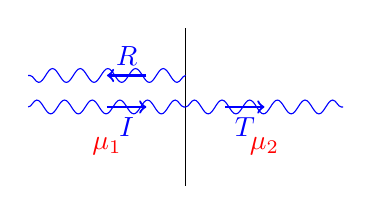
\begin{tikzpicture}
        \draw (0, -1) -- (0, 1);
        \draw [blue,decorate, decoration=snake] (-2, 0) -- (0,0);
        \draw [blue,decorate, decoration=snake] (0, 0.4) -- (-2,0.4);
        \draw [blue,decorate, decoration=snake] (0, 0) -- (2,0);
        \draw [blue, ->, thick] (-1, 0) -- node[below]{$I$} (-0.5,0);
        \draw [blue, ->, thick] (0.5, 0) -- node[below]{$T$} (1,0);
        \draw [blue, ->, thick] (-0.5, 0.4) -- node[above]{$R$} (-1,0.4);
        \draw [red] (-1, -0.5) node[]{$\mu_1$};
        \draw [red] (1, -0.5) node[]{$\mu_2$};
    \end{tikzpicture}
\end{center}

\[ y_I\br{x,t} = A_I \sin \br{k_1 \br{x - v_1 t}} \]
\[ y_R\br{x,t} = A_R \sin \br{k_1 \br{x + v_1 t}} \]
\[ y_T\br{x,t} = A_T \sin \br{k_2 \br{x - v_2 t}} \]
\textbf{a)}
\[ \w_1 = \w_2 \implies k_1 v_1 = k_2 v_2 \]
This means that the ``knot'' at the interface is a ``good'' knot -- i.e. the string at either side of the interface ($x=0$) move with the same frequency -- i.e. the strings are connected.\\

\textbf{b)}

\begin{center}
    \begin{tikzpicture}
        \draw[fill] (0,0) circle (0.05);
        \draw[thick,->] (0,0) -- (1,1) node[above right]{$\ve F_2$};
        \draw[thick,->] (0,0) -- (-1,-0.6) node[below left]{$\ve F_1$};
    \end{tikzpicture}
\end{center}

\[ m \ve a\tsb{net} = \ve F_1 + \ve F_2 \]
If the slopes are the same then $\ve F_1 \parallel \ve F_2$ and so $\ve a\tsb{net}$ is also parallel.

\begin{center}
    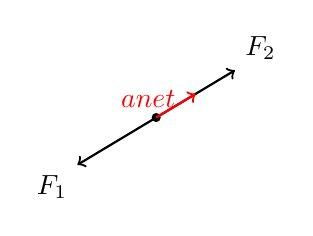
\begin{tikzpicture}
        \draw[fill] (0,0) circle (0.05);
        \draw[red] (-0.1,0) node[above]{$\ve a\tsb{net}$};
        \draw[thick,->] (0,0) -- (1,0.6) node[above right]{$\ve F_2$};
        \draw[thick,->] (0,0) -- (-1,-0.6) node[below left]{$\ve F_1$};
        \draw[thick,red, ->] (0,0) -- (0.5,0.3);
    \end{tikzpicture}
\end{center}
By the principle of superposition the equations for the waves in the first medium can be simply added together,
\[ y_1 \br{x,t} = y_I\br{x,t} + y_R\br{x,t} \]
\[ y_2 \br{x,t} = y_T\br{x,t} \]
Introduce the constraints of a good string,
\[ y_1\br{x=0, t} = y_2\br{x=0, t} \]
Therefore,
\[ A_I \sin\br{-k_1 v_1 t} + A_R \sin\br{k_1 v_1 t} = A_T \sin\br{-k_2 v_2 t} \]
Therefore,
\[ - A_I + A_R = - A_T \]
Equivalently,
\[ A_I = A_R + A_T \]
\textbf{d)}
The next constraint imposes,
\[ \pder{}{x}y_1\br{x=0, t} = \pder{}{x}y_2\br{x=0, t} \]
\[ k_1A_I \cos\br{-k_1 v_1 t} + k_1A_R \cos\br{k_1 v_1 t} = k_2A_T \cos\br{-k_2 v_2 t} \]
Thus,
\[ k_1 A_I + k_2 A_R = k_2 A_T \]
Now solve for the reflected and transmitted $A_R, A_T$ in terms of the given incidence amplitude. So,
\[ A_R = \f{v_1 - v_2}{v_1 + v_2} A_I \]
\[ A_T = \f{2v_2}{v_1 + v_2} A_I \]
\textbf{e)}
If $v_2 > v_1$ then $A_R \propto - \br{A_I}$.

\subsection{Polarization}
So far, we have only considered 1D waves. However, the electric and magnetic fields are vector quantities. As we shall see shortly, EM radiation has field components that are perpendicular to the direction of propagation. We can thus write a traveling wave as
\[ \ti {\ve f}\br{z, t} = \ti f_{k} \hat n e^{i\br{kz - \w t}} \]
Where $e^{i\br{kz - \w t}}$ acts as the traveling wave, $\hat n$ is the polarization and $\ti f_{k}$ is the amplitude and phase. Note that $\ti f_{k}$ is not a function of position $\ve r$ and time $t$. The possible polarizations of this plane wave are $\hat x, \hat y$ or a linear combination thereof. An important linear combination is,
\[ \hat n_{\pm} = \hat x \pm i \hat y = \hat x \pm e^{i \pi / 2} \hat y \]
So that,
\[ \hat n_{\pm} e^{i\br{kz - wt}} = \hat x e^{i\br{kz - wt}} \pm \hat y e^{i\br{kz - wt + \pi/2}}\]
Which makes the total wave,
\begin{align*}
\Re\bc{\ti f_{k}\hat n_{\pm} e^{i\br{kz - wt}}}
&= \Re\bc{\abs{\ti f_{k}} e^{i \de} \hat n_{\pm} e^{i\br{kz - wt}}} \\
&= \abs{\ti f_{k}}\Re\bc{\br{\hat x + i \hat y} \br{\cos \br{kz - wt + \de} + i\sin \br{kz - wt + \de}}} \\
&= \abs{\ti f_{k}}\br{\hat x \cos \br{kz - wt + \de} - \hat y\sin \br{kz - wt + \de}} \\
\end{align*}

\begin{center}
    \begin{tikzpicture}
        \pgfmathsetmacro\rs{1.5}
        \draw (-2, 0) -- (2, 0) node[right]{$x$};
        \draw (0, -2) -- (0, 2) node[above]{$y$};
        \draw[red, ->] (0,0) -- (\rs, 0) node[above right]{$t = 0$};
        \draw[green, ->] (0,0) -- ({cos(60)*\rs}, {sin(60)*\rs}) node[above right]{$t = 2\De t$};
        \draw[green, ->] (0,0) -- ({cos(90)*\rs}, {sin(90)*\rs}) node[above]{$t = 3\De t$};
        \draw[green, ->] (0,0) -- ({cos(30)*\rs}, {sin(30)*\rs}) node[above right]{$t = \De t$};
    \end{tikzpicture}
\end{center}

\subsection{EM Plane Waves}
While this is sufficient for a generic wave equation however, for those satisfying Maxwell's Equations there are further conditions to impose. In particular, for a plane wave traveling in the $z$-direction we have,
\[ \ti {\ve E} \br{z, t} = \ti{\ve E}_0 e^{i\br{k z - \w t}} \]
With derivatives,
\[ \pder{}{x} \ti {\ve E} = \pder{}{y} \ti {\ve E} = \ve 0 \]
\[ \pder{}{z} \ti {\ve E} = ik \ti {\ve E} \]
\[ \pder{}{t} \ti {\ve E} = -i\w \ti {\ve E} \]
We will write,
\[ \ti{{\ve E}}_0 = \hat x \ti {E}_{0, x} + \hat y \ti {E}_{0, y} + \hat z \ti {E}_{0, z} \]
And similarly for the magnetic field,
\[ \ti {\ve B}_0 = \hat x \ti {B}_{0, x} + \hat y \ti {B}_{0, y} + \hat z \ti {B}_{0, z} \]
Note that this is not the same as the electric field itself,
\[ \ti E_x = \ti{\ve E} \cdot \hat x = \ti{\ve E}_0 \cdot \hat x e^{i \br{kz - \w t}} = \ti{E}_{0,x} e^{i \br{kz - \w t}} \]
Next make use of Gauss's law (in vacuum),
\[ 0 = \vdel \cdot \ve E = \ti E_{0,z} i k e^{i\br{kz - \w t}} \implies \ti E_{0,z} = 0 \]
Similarly for $\ve B$,
\[ \ti B_{0,z} = 0 \]
So that EM waves are \textit{transverse} and $\ti {\ve E}_0$ only has components in the $\hat x$ and $\hat y$ directions.\\

Moreover make use of Faraday's law,
\[ \vdel \times \ve E = - \pder{\ve B}{t} \]
Which gives,
\[ - i k \hat x \ti E_y + i k \hat y \ti E_x = i \w \br{ \hat x \ti B_x + \hat y \ti B_y + \hat z \ti B_z} \]
Therefore matching components,
\begin{align*}
    -i k \ti E_y &= i \w \ti B_x \\
    i k \ti E_x &= i \w \ti B_y \\
    0 &= i \w \ti B_z
\end{align*}
Which makes,
\begin{align*}
    \ti E_y &= - \f{\w}{k} \ti B_x = - c \ti B_x \\
    \ti E_x &= + \f{\w}{k} \ti B_y = + c \ti B_y
\end{align*}
And so $\ti{\ve E}$ and $\ti{\ve B}$ have the same phase but are in the different directions. In this case, we can write $c \ti{\ve B} = \hat z \times \ti{\ve E}$ so that the set $\bc{\ti{\ve E} , \ti{\ve B} , \hat z}$ form a right-hand set (which was already known from $\mu_0 \ve S = \ve E \times \ve B$). We can generalize this to a plane wave traveling in an arbitrary direction by introducing the \term{wave vector} $\ve k = k_x \hat x + k_y \hat y + k_z \hat z$. Also,
\[ \ve k = k \hat k = \sqrt{k_x^2 + k_y^2 + k_z^2} \hat k \]
The recurring relation $k z - \w t$ becomes,
\[ \ve k \cdot \ve r - \w t  \]
Monochrome plane waves in vacuum traveling in the $\hat k$ direction are,
\begin{align*}
\ti{\ve E}\br{\ve r , t} &= \ti{\ve E}_0 e^{i\br{\ve k \cdot \ve r - \w t}} \\
c\ti{\ve B}\br{\ve r , t} &= \hat k \times \ti{\ve E}\br{\ve r , t}
\end{align*}
The quantity $\ti{\ve E}_0 = \hat x \ti{E}_{0,x} + \hat y \ti{E}_{0,y} + \hat z \ti{E}_{0,z} = \hat n E_0 e^{i \de}$ represents the polarization, amplitude, and phase of the wave but contains no space or time dependence.
\subsection{Energy and Momentum}
We are now equipped with the general setting of a monochromatic plane wave traveling in a direction $\hat k$. It has already been seen that $\hat k$ is in the same direction as the Poynting vector $\ve S$ which points in the direction of electromagnetic radiation. $\ve S$ satisfies Poynting's theorem,
\[ \vdel \cdot \ve S + \pder{u}{t} + \ve E \cdot \ve J = 0 \]
Which in a vacuum indicates that $\ve S \cdot \dif \ve a$ is the amount of energy flowing out of a point in a time $\dif t$. Therefore the electromagnetic waves previously discussed are carrying electromagnetic energy. The electromagnetic energy density is,
\[ u = \f{\ep_0}{2}E^2 + \f{1}{2 \mu_0} B^2 \]
But for electromagnetic waves, $B^2 = \mu_0 \ep_0 E^2$. Thus
\begin{align*}
    u = \f{\ep_0}{2} E^2 + \f{1}{2\mu_0} \mu_0 \ep_0 E^2 = \ep_0 E^2
\end{align*}
Which for a monochromatic 1D wave becomes,
\[  u = \ep_0 E_0^2 \cos^2\br{kz - \w t + \de} \]
At a point $z$ at time $t$ there is local energy density of $u\br{z,t}$ stored in the electromagnetic field. The Poynting vector however is,
\[ \ve S = \f{1}{\mu_0} \ve E \times \ve B = \f{1}{\mu_0} \ve E \times \br{\f{1}{c} \ve k \times \ve E} \]
Which by a triple product vector identity $\ve A \times \br{\ve B \times \ve C} = \ve B \br{\ve A \cdot \ve C} - \ve C \br{\ve A \cdot \ve B}$ yields,
\[ \ve S = \f{1}{c \mu_0} \bs{\ve k E^2 - \ve E \br{\ve E \cdot \ve k}} \]
But $\ve k$ is orthogonal to $\ve E$,
\[ \ve S = \f{1}{c\mu_0} E^2 \ve k = c\ep_0 E^2 \ve k = c u \ve k \]
This is remarkable. The Poynting vector indicates that there is a flow of energy per unit area per unit time of $c u$ in the $\ve k$ direction.

\subsection{Electromagnetic Waves in Media}

Heretofore, we have studied electromagnetic fields in the vacuum of space. In materials/media that are linear, isotropic and homogeneous (LIH) there are few modifications that need to be made. The electric polarization $\ve P$ is,
\[ \ve P = \chi \ve D \]
Such that the total electric field is $\ve E = \ve P + \ve D$. Inside a dielectric (where there is no free charge), Maxwell's equations are,
\begin{align*}
    \vdel \cdot \ve D &= 0 \\
    \vdel \cdot \ve B &= 0 \\
    \vdel \times \ve E &= - \pder{\ve B}{t} \\
    \vdel \times \ve H &= \pder{\ve D}{t}
\end{align*}

For LIH materials, we define $\ve D = \ep \ve E$ and $\ve H = \f{1}{\mu} \ve B$ such that,
\begin{align*}
    \vdel \cdot \ve E &= 0 \\
    \vdel \cdot \ve B &= 0 \\
    \vdel \times \ve E &= - \pder{\ve B}{t} \\
    v^2 \vdel \times \ve B &= \pder{\ve E}{t}
\end{align*}

Where $v^2 = 1 / \ep \mu$ is the speed of light in the medium.

\[ c = \f{1}{\sqrt{\ep_0 \mu_0}} \mapsto v = \f{1}{\sqrt{\ep \mu}} \]

As such, Maxwell's equations in LIH materials are nearly identical; the only necessary modification is to replace the speed of propagation $c$ with a speed $v$ that is dependent on the material. \\

In a higher level course, one would explore how to modify Maxwell's equations for materials that do not obey the assumptions of linearity, isotropy, and homogeneity. Doing so is of great importance; material sciences are a very versatile field of physics with countless applications. \\

If one has a dielectric media adjacent to vacuum and a light source emanating isotropically, there are two contributions to light incident on an observer sitting on the interface: the source ray, and the ray reflected off the vacuum dielectric interface.

\begin{center}
    \begin{tikzpicture}
        \draw[] (-3, 0) -- (3,0);
        \draw (3,2) node[](source){$S$};
        \draw (-2,0.5) node[](obs){$O$};
        \coordinate (r) at (-0.2,0);
        \begin{scope}[decoration={markings, mark=at position 0.5 with {\arrow{>}}}]
            \draw[thick, postaction={decorate}] (source) -- node[below right]{$\ve k$} (r);
            \draw[thick, postaction={decorate}] (r) -- (obs);
            \draw[thick, postaction={decorate}] (source) -- (obs);
            \draw[dashed, thick, postaction={decorate}] (r) -- (-1.6, -1);
        \end{scope}
        \draw (2,0) node[above right]{Vacuum};
        \draw (2,0) node[below right]{Dielectric};
        \draw (r) -- (-0.2, 2);
        \draw (-0.2, 0.2) node[above left]{$\te_{R}$};
        \draw (-0.2, 0.2) node[above right]{$\te_{I}$};
    \end{tikzpicture}
\end{center}

The reflected ray is polarized horizontally upon reflecting off the surface of the medium.

\subsection{Conductors}

Inside a conductor we have,
\[ \ve J_f = \si \ve E \eq \label{eq:ohms_law}\]
Where $\si$ is the conductivity, $\ve J_f$ is the free current density and $\ve E$ is the electric field. More generally $\si$ can be a tensor that has components for every pair of directions. However for homogeneous and isotropic media, we can take the conductivity to be a scalar quantity. In contrast, the bound current density $\ve J_b$ is the set of moving charges that are bound to atoms in the material. Specifically the \textit{ensemble} of electrons bound orbitally to atoms contribute a current that flows through the medium (typically surface currents).\\

\Cref{eq:ohms_law} is called \term{Ohm's law}. Ohm's law is typically introduced as $V = IR$. The $V = IR$ equation is a consequence of the local equation that is \cref{eq:ohms_law} together with the assumptions of homogeneity and isotropy. \\

Recall that for constant electric fields, Ohm's law holds initially. However, the electric field with polarize the material to the point where the internal induced electric field exactly cancels the applied electric field. The system approaches equilibrium. \\

However for time depended electric fields, the material's polarization with be a function of time as well. Considering the applied field as an oscillation at frequency $f$, the material's amplitude of oscillation will peak at its resonant frequency. Moreover, there will be a phase shift at the resonant frequency as well.

\subsection{Absorption \& Dispersion}

Inside a conductor we have $\ve J_f = \si \ve E$ where $\si$ is the conductivity (resistivity is $1/\rho$). In order to determine how the wave equations are modified, first begin with Ampère's circuital law,
\[ \vdel \times \ve B = \mu_0 \ve J + \mu_0 \ep_0 \pder{\ve E}{t} \]
In materials this law becomes,
\[ \vdel \times \ve B = \mu \ve J_f + \mu \ep \pder{\ve E}{t} \]
Which can be written,
\[ v^2 \vdel \times \ve B = \f{1}{\ep} \ve J_f + \pder{\ve E}{t} \]
Now make use of Ohm's law for conductors ($\ve J = \si \ve E$) to arrive at,
\[ v^2 \vdel \times \ve B = \f{\si}{\ep} \ve E + \pder{\ve E}{t} \eq \label{eq:ampere}\]
Faraday's law gives us the useful relationship,
\[ \vdel\br{\vdel \cdot \ve E} - \del^2 \ve E = \vdel \times \br{\vdel \times \ve E} = - \pder{}{t}\br{\vdel \times \ve B} \eq \label{eq:faraday} \]
But we have that $\vdel \cdot \ve E = \f{1}{\ep} \rho_{f}$. In a conductor $\rho_{f} \approx 0$ because the time scale to equilibrate $\tau_{d} = \f{\ep}{\si} \approx \SI{1e-20}{\s}$ is short (of course if your frequency is $f \geq \tau_d^{-1}$ this approximation doesn't hold). Making the conductive approximation that $\vdel \cdot \ve E \propto \rho_f \approx 0$ makes a solution more conducive. Substitute \cref{eq:faraday} into \cref{eq:ampere},
\[ v^2 \del^2 \ve E = \f{\si}{\ep} \pder{\ve E}{t} + \pdder{\ve E}{t} \eq \label{eq:wave_dispersion} \]
Therefore we arrive at,
\[ v^2 \del^2 \ve E = \pdder{\ve E}{t} + \f{\si}{\ep} \pder{\ve E}{t} \]
Which suggests the ansatz solution $\ve E = \Re\br{\ti{\ve E}}$ where,
\[ \ti{\ve E} \br{\ve r, t} = \ti{\ve E}_0 e^{i\br{\ti{\ve k}\cdot \ve r - \w t}} = \ti{\ve E}_0 e^{i\br{\ti{k}_x x + \ti{k}_y y + \ti{k}_z z - \w t}} \eq \label{eq:ansatz}\]
Where $\ti{\ve k} \in \C^3$. If \cref{eq:ansatz} is to solve \cref{eq:wave_dispersion} then,
\begin{align*}
    \del^2 \ti{\ve E} &= \br{-\ti{k}_x^2 -\ti{k}_y^2 -\ti{k}_z^2} \ti{\ve E} = -\ti{\ve k}\cdot\ti{\ve k} \ti{\ve E}\\
    \pder{\ti{\ve E}}{t} &= -i\w \ti{\ve E}_0 e^{i\br{\ti{\ve k}\cdot \ve r - \w t}} = - i\w \ti{\ve E} \\
    \pdder{\ti{\ve E}}{t} &= -\w^2 \ti{\ve E}
\end{align*}
Therefore,
\[ v^2 \ti{\ve k}\cdot\ti{\ve k} \ti{\ve E} = \f{\si}{\ep} i\w \ti{\ve E} + \w^2 \ti{\ve E} \]
Assuming the trivial solution $\ti{\ve E}$ is not permitted,
\[ \ti{\ve k}\cdot\ti{\ve k} = i \mu \si \w + \mu \ep \w^2 \eq \label{eq:aux}\]
Which is the auxiliary equation for materials. Let $\ti{\ve k} = \ti{k} \hat k = \Re\br{\ti{k}} \hat k + i\Im\br{\ti{k}} \hat k$. Now introduce the real part of $\ti{k}$ to be simply $k$ and $\kappa$ to be the imaginary part,
\begin{align*}
\ti{\ve k}\cdot\ti{\ve k}
&= \br{\ti{k}}^2 \\
&= \br{\Re\br{\ti{k}} + i\Im\br{\ti{k}}}^2 \\
&= \br{k + i\kappa}^2 \\
&= k^2 - \kappa^2 + 2i k \kappa
\end{align*}
Making real and imaginary parts of \cref{eq:aux},
\begin{align*}
    2 k \kappa &= \mu \si \w \eq \label{eq:1_imaginary_match}\\
    k^2 - \kappa^2 &= \mu \ep \w^2 \eq \label{eq:1_real_match}
\end{align*}
Squaring \cref{eq:1_imaginary_match} and subbing in \cref{eq:1_real_match},
\[ \mu^2 \si^2 \w^2 = 4 k^2 \kappa^2 = 4 k^2 \br{k^2 - \mu \ep \w^2}  \]
\[ 0 = k^4 - \mu \ep \w^2 k^2 - \f14\mu^2 \si^2 \w^2  \]
Which can be solved using the quadratic equation,
\begin{align*}
k^2
&= \f{\mu \ep \w^2 \pm \sqrt{\br{\mu \ep \w^2}^2 + 4\br{\f14\mu^2 \si^2 \w^2}}}{2} \\
&= \f{\mu \ep \w^2 \pm \mu \ep \w^2 \sqrt{1 + \br{\f{\si}{\w\ep}}^2}}{2} \\
&= \f{\mu \ep \w^2}{2}\bc{1 \pm \sqrt{1 + \br{\f{\si}{\w\ep}}^2}} \\
&= \f{\mu \ep \w^2}{2}\bc{1 + \sqrt{1 + \br{\f{\si}{\w\ep}}^2}} \note{Assert that $k \in \R$} \eq \label{eq:quad_solve}\\
\end{align*}
Therefore,
\[ k = \w \sqrt{\f{\mu \ep}{2}}\sqrt{1 + \sqrt{1 + \br{\f{\si}{\w\ep}}^2}} \]
As required. \cref{eq:1_real_match} immediately forces $\kappa$ to be,
\[ \kappa = \w \sqrt{\f{\mu \ep}{2}}\sqrt{-1 + \sqrt{1 + \br{\f{\si}{\w\ep}}^2}} \]

In order to solve \cref{eq:wave_dispersion} we first need to define boundary conditions. Consider the interface of a conductor and a vacuum, Maxwell's equations in a conductor are,
\begin{align*}
    \vdel \cdot \ve D &= \rho_f \\
    \vdel \cdot \ve B &= 0 \\
    \vdel \times \ve E &= - \pder{\ve B}{t} \\
    \vdel \times \ve H &= \ve J_f + \pder{\ve D}{t}
\end{align*}

At the interface we can consider the usual pill-box domain $\s V$,
\[ \int_{\s V} \vdel \cdot \ve D \dif \tau = \oint_{\di \s V} \ve D \cdot \dif \ve a = \int_{\s V} \rho_f \dif \tau = Q \]
When placed on the interface we arrive at the first boundary condition,
\[ \ep_1 E_1^{\perp} - \ep_2 E_2^{\perp} = \si_f \]
Next consider a loop $\di \s A$ across the surface,
\[ \int_{\di \s A} \ve E \cdot \dif \ve \ell = \int_{\s A} \vdel \times \ve E \cdot \dif \ve a = - \dot \Phi_m = 0  \]
Therefore we arrive at the second boundary condition,
\[ \ve E_1^{\parallel} - \ve E_{2}^{\parallel} = 0 \]
There are analogously boundary conditions for the magnetic field,
\[ B_1^{\perp} - B_2^{\perp} = 0 \]
\[ \f{1}{\mu_1}\ve B_1^{\parallel} - \f{1}{\mu_2}\ve B_2^{\parallel} = \ve K_f \times \hat n \]

If we consider a wave incidence on a conductor with normal in the $\hat z$ direction,
\begin{center}
    \begin{tikzpicture}
        \draw (-3, 0) -- (3, 0);
        \coordinate (o) at (0, 0);
        \coordinate (I) at (-1, 2);
        \coordinate (R) at (1, 2);
        \begin{scope}[decoration={markings, mark=at position 0.5 with {\arrow{>}}}]
            \draw[thick, postaction={decorate}] (I) -- node[left]{$\ve k_I$} (o);
            \draw[thick, postaction={decorate}] (o) -- node[right]{$\ve k_R$} (R);
        \end{scope}
        \draw[->] (I) -- ($(I) + (0.5, 0.25)$) node[above]{$\ve E_I$};
        \draw[->] (R) -- ($(R) + (-0.5, 0.25)$) node[above]{$\ve E_R$};
        \draw[dashed] (o) -- ($(o) + (0, 3)$);
        \draw ($(o) + (-0.2, 1)$) node[]{$\te$};
        \draw (2, 0) node[above]{vacuum};
        \draw (2, 0) node[below]{conductor};
    \end{tikzpicture}
\end{center}

Let the incidence plane wave (in region $1$) be monochrome with wave-vector $\ve k_I$,
\begin{align*}
    \ti {\ve E}_I\br{\ve r, t} &= \ti {\ve E}_{I,0} e^{i\br{\ve k_I \cdot \ve r - \w t}} \\
    \ti {\ve B}_I\br{\ve r, t} &= \f{1}{v_{1}} \br{\hat k_I \times \ti {\ve E}_I}
\end{align*}
Analogously for the reflected and transmitted waves,
\begin{align*}
    \ti {\ve E}_R\br{\ve r, t} &= \ti {\ve E}_{R,0} e^{i\br{\ve k_R \cdot \ve r - \w t}} \\
    \ti {\ve B}_R\br{\ve r, t} &= \f{1}{v_{1}} \br{\hat k_R \times \ti {\ve E}_R} \\
    \ti {\ve E}_T\br{\ve r, t} &= \ti {\ve E}_{T,0} e^{i\br{\ve k_T \cdot \ve r - \w t}} \\
    \ti {\ve B}_T\br{\ve r, t} &= \f{1}{v_{2}} \br{\hat k_T \times \ti {\ve E}_T}
\end{align*}
At the interface (say $z = 0$) Maxwell's equations induce boundary conditions such that components of the fields in region $1$ must match the fields in region $2$,
\begin{align*}
    \eq \label{eq:boundary1}
    \begin{split}
    \ti {E}_{I; x,y}\br{z=0, t} + \ti {E}_{R; x,y}\br{z=0, t} &= \ti {E}_{T; x,y}\br{z=0, t}  \\
    \ti {B}_{I; z}\br{z=0, t} + \ti {B}_{R; z}\br{z=0, t} &= \ti {B}_{T; z}\br{z=0, t}
    \end{split}
\end{align*}
Moreover their derivatives must match,
\begin{align*}
    \eq \label{eq:boundary2}
    \begin{split}
   \pder{}{\chi} \ti {E}_{I;x,y}\br{z=0, t} + \pder{}{\chi}\ti {E}_{R;x,y}\br{z=0, t} &= \pder{}{\chi}\ti {E}_{T;x,y}\br{z=0, t}  \\
    \pder{}{\chi}\ti {B}_{I;z}\br{z=0, t} + \pder{}{\chi}\ti {B}_{R;z}\br{z=0, t} &= \pder{}{\chi}\ti {B}_{T;z}\br{z=0, t}
    \end{split}
\end{align*}
Where $\chi \in x,y,z,t$. Therefore \cref{eq:boundary1} gives,
\[ \ti {\ve E}_{I;0} e^{i\br{x k_{I;x} + y k_{I;y} - \w t}} + \ti {\ve E}_{R;0} e^{i\br{x k_{R;x} + y k_{R;y} - \w t}} = \ti {\ve E}_{T;0} e^{i\br{x k_{T;x} + y k_{T;y} - \w t}} \quad (z=0, x) \]
Since \cref{eq:boundary1} must be satisfied for all space and time, set $x=y=t=0$ to obtain,
\[ \ti {\ve E}_{I;0} + \ti {\ve E}_{R;0} = \ti {\ve E}_{T;0}  \quad (z=0) \eq \label{eq:direction_sum}\]
More explicitly, set $x=y=t=0$ and $\chi = t$ in \cref{eq:boundary2} to obtain,
\[ -i\w\ti {\ve E}_{I,0} + -i\w\ti {\ve E}_{R,0} = -i\w\ti {\ve E}_{T,0}  \quad (z=0) \]
This acts as confirmation that the frequency of all three wave $\w$ is fixed by the source. Therefore,
\[ \w = k_I v_{1}= k_R v_{1}= k_T v_{2} \eq \label{eq:vv}\]
Similarly set $x = y = t = 0$ and $\chi = y$,
\[ ik_{I;y}\ti {\ve E}_{I,0} + ik_{R;y}\ti {\ve E}_{R,0} = ik_{T;y}\ti {\ve E}_{T,0}  \quad (z=0) \]
Any resolution between this and \cref{eq:direction_sum} requires,
\[ k_{I;y} = k_{R;y} = k_{T;y} \eq \label{eq:wavey} \]
Similarly for $x$,
\[ k_{I;x} = k_{R;x} = k_{T;x} \eq \label{eq:wavex} \]
For convenience (and without loss of generality), place all wave-vectors in the $x,z$-plane.
\[ k_{I;y}= k_{R;y} = k_{T;y} = 0 \]
Then we have,
\[ \tan \te_i = \f{k_{i; z}}{k_{i; x}} \quad \forall i \in I, T, R \]
Where the following relationships must hold (as a consequence of \cref{eq:wavex,eq:wavey,eq:vv}),
\[ k_R = k_I \]
\[ k_T\f{v_2}{v_1} = k_T\f{n_1}{n_2} = k_I \]
\[ k_{I}\cos\te_{I} = k_{R}\cos\te_{R} = k_{T}\cos\te_{T} \]
\[ k_{I}\sin\te_{I} = k_{R}\sin\te_{R} = k_{T}\sin\te_{T} \]
\[ \te_I = \te_R \eq \label{eq:ir}\]
\[ \f{\sin\te_{T}}{\sin\te_{I}} = \f{n_1}{n_2} \eq \label{eq:snell}\]
The remaining boundary conditions reduce to (at $z=0$),
\begin{align*}
    \eq \label{eq:b1}\ep_{1} \ti {E}_{I, 0; z} + \ep_{1} \ti {E}_{R, 0; z} &= \ep_{2} \ti {E}_{T, 0; z} \\
    \eq \label{eq:b2}\ti {E}_{I, 0; x,y} + \ti {E}_{R, 0; x,y} &= \ti {E}_{T, 0; x,y} \\
    \eq \label{eq:b3}\ti {B}_{I, 0; z} + \ti {B}_{R, 0; z} &= \ti {B}_{T, 0; z} \\
    \eq \label{eq:b4}\f{1}{\mu_1}\ti {B}_{I, 0; x,y} + \f{1}{\mu_1}\ti {B}_{R, 0; x,y} &= \f{1}{\mu_2}\ti {B}_{T, 0; x,y}
\end{align*}
The reflection and transmission coefficients are defined as,
\begin{align*}
    R &= \f{I_R}{I_I} = \br{\f{\ti E_{R,0}}{\ti E_{I,0}}}^2 \\
    T &= \f{I_T}{I_I} = \f{\ep_2 v_2}{\ep_1 v_1}\br{\f{\ti E_{T,0}}{\ti E_{I,0}}}^2 \f{\cos \te_T}{\cos \te_I}
\end{align*}

\subsubsection{Parallel Incidence}

Up until this point, the polarizations $\ti {\ve E}_{I, 0}, \ti {\ve B}_{I, 0}$ have been assumed arbitrary. In order to solve the boundary conditions \cref{eq:b1,eq:b2,eq:b3,eq:b4}, assume that the polarization is \textit{parallel} to the incidence plane. Namely,
\[ \ti {\ve E}_{i, 0} = \ti {E}_{i, 0; x} \hat x + \ti {E}_{i, 0; z} \hat z \quad \forall i \in I, R, T\eq \label{eq:parallel}\]
Where,
\begin{align*}
    \ti {E}_{I, 0; x} &= \ti {E}_{I, 0} \cos \te_I \\
    \ti {E}_{I, 0; z} &= \ti {E}_{I, 0} \sin \te_I
\end{align*}
Using this, \cref{eq:b2} claims that,
\[ \ti E_{I,0} \cos \te_I + \ti E_{R,0} \cos \te_R = \ti E_{T,0} \cos \te_T\]
But \cref{eq:ir} reveals that $\te_I = \te_R$,
\[ \ti E_{I,0} + \ti E_{R,0}  = \ti E_{T,0} \f{\cos \te_T}{\cos \te_I}\]
Moreover \cref{eq:b1} yields,
\[ -\ep_1\ti E_{I,0} \sin \te_I + \ep_1\ti E_{R,0} \sin \te_R = -\ep_2\ti E_{T,0} \sin \te_T \eq \label{eq:parallel_B1}\]
Where the negative signs are present because $\ti {\ve E}_{I,0}$ and $\ti {\ve E}_{T,0}$ point in the $+z$-direction while $\ti {\ve R}_{I,0}$ points in the $-z$-direction.
Notice that \cref{eq:b3} is already satisfied at $z=0$. All that remains is to solve is \cref{eq:b4}. Beginning with \cref{eq:b4} and $\ti {\ve B}_{i, 0} = \f{1}{v_i} \hat k_{i} \times \ti {\ve E}_{i, 0}$,
\[ \ti {B}_{i, 0;l} = \ep_{mnl} \f{1}{v_i} k_{i;m} \ti {E}_{i, 0;n} \]
As an example $l = x$,
\begin{align*}
\ti {B}_{i, 0;x} &= \ep_{mnx} \f{1}{v_i} k_{i;m} \ti {E}_{i, 0;n} \\
&= \ep_{yzx} \f{1}{v_i} \underbrace{k_{i;y}}_{0} \ti {E}_{i, 0;z} + \ep_{zyx} \f{1}{v_i} k_{i;z} \underbrace{\ti {E}_{i, 0;y}}_{0} \\
&= 0 \\
\end{align*}
By geometry, $\ti {\ve E}_{i, 0}$ and $\hat k_i$ are in the same $x,z$-plane. Therefore the only non-zero components of $\ve B$ is perpendicular to the $x,z$-plane. Namely,
\begin{align*}
\ti {\ve B}_{i, 0}
&= \ti {B}_{i, 0}\hat{y} \\
&= \ep_{mny} \f{1}{v_i} k_{i;m} \ti {E}_{i, 0;n}\hat{y} \\
&= \br{\ep_{xzy} \f{1}{v_i} k_{i;x} \ti {E}_{i, 0;z} + \ep_{zxy} \f{1}{v_i} k_{i;z} \ti {E}_{i, 0;x}}\hat{y} \\
&= \br{- \f{1}{v_i} k_{i;x} \ti {E}_{i, 0;z} + \f{1}{v_i} k_{i;z} \ti {E}_{i, 0;x}}\hat{y} \\
&= \bc{- k_{i;x} \sin\br{\te_i} + k_{i;z} \cos\br{\te_i}}\f{1}{v_i}\ti {E}_{i, 0}\hat{y}\\
&= \bc{k_{i;x}^2 + k_{i;z}^2}\f{1}{v_i}\ti {E}_{i, 0}\hat{y} \\
&= \f{1}{v_i}\ti {E}_{i, 0}\hat{y}
\end{align*}
Therefore \cref{eq:b4} becomes,
\[ \f{1}{\mu_1}\ti {B}_{I, 0; y} + \f{1}{\mu_1}\ti {B}_{R, 0; y} = \f{1}{\mu_2}\ti {B}_{T, 0; y} \]
\[ \f{1}{\mu_1v_1}\br{\ti E_{I, 0} - \ti E_{R, 0}} = \f{1}{\mu_2 v_2} \ti E_{T, 0} \]
\[ \ti E_{I, 0} - \ti E_{R, 0} = \f{\mu_1 v_1}{\mu_2 v_2} \ti E_{T, 0} \]
This is identical to \cref{eq:parallel_B1}. Define $\al, \be$ such that,
\[ \al = \f{\cos \te_T}{\cos \te_I} = \f{\sqrt{1 - \bs{\br{n_1 /n_2} \sin \te_I}^2}}{\cos \te_I} \qquad \be = \f{\mu_1 v_1}{\mu_2 v_2} \]
Which gives the amplitudes as Fresnel's equations,
\[ \ti E_{R,0} = \br{\f{\al - \be}{\al + \be}} \ti E_{I,0} \quad \ti E_{T,0} = \br{\f{2}{\al + \be}} \ti E_{I,0} \eq \label{eq:fresnel_parallel}\]
As a sanity check, at normal incidence ($\te_I = 0$),
\[ \al = \f{\sqrt{1 - \bs{\br{n_1 / n_2} \sin \br{0}}^2}}{\cos \br{0}} = 1 \]

\term{Brewster's angle} $\te_B$ is the special angle at which all transmitted waves go to zero. This occurs when $\f{\ti E_{R,0}}{\ti E_{I,0}} = 1$. This occurs when $\al\br{\te_B} = \be$,
\[ \f{\sqrt{1 - \bs{\br{n_1 /n_2} \sin \te_B}^2}}{\cos \te_B} = \f{\mu_1 v_1}{\mu_2 v_2} = \be \]
\[ 1 - \bs{\br{n_1 /n_2} \sin \te_B}^2 = \cos^2 \te_B\be^2 \]
\[ 1 - \f{n_1^2}{n_2^2}\sin^2 \te_B = \be^2 - \sin^2 \te_B\be^2 \]
\[ \sin^2 \te_B = \br{\be^2 - 1}\br{\be^2 - \f{n_1^2}{n_2^2}}^{-1}  \]
The reflected and transmitted amplitudes become equal at $\te_C$ when $\al - \be \approx 2$
\[ \f{\sqrt{1 - \bs{\br{n_1 /n_2} \sin \te_C}^2}}{\cos \te_C} - \be = 2\]
Using the previous analysis $\be \mapsto 2 + \be$,
\[ \f{\sqrt{1 - \bs{\br{n_1 /n_2} \sin \te_C}^2}}{\cos \te_C} = 2 + \be\]
\[ \sin^2 \te_C = \br{\br{2+ \be}^2 - 1}\br{\br{2+ \be}^2 - \f{n_1^2}{n_2^2}}^{-1}\]
For typical values,
\begin{center}
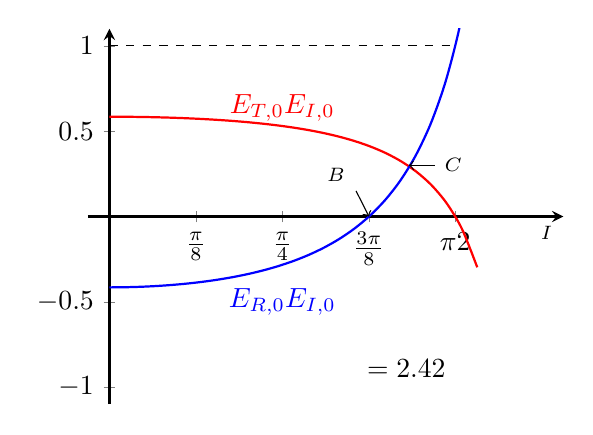
\begin{tikzpicture}
        \pgfmathsetmacro\ben{2.42}
        \pgfmathsetmacro\ls{0.15}
        \begin{axis}[
            standardplot,
            xmin=0, xmax=5, ymin=-1, ymax=1,
            xlabel={$\te_I$},
            domain=0:4,
            range=-1:1,
            xtick={0,1,2,3,4},
            xticklabels={$0$,$\frac{\pi}{8}$,$\frac{\pi}{4}$,$\frac{3\pi}{8}$,$\f{\pi}{2}$},
            ytick={-1,-0.5,0,0.5,1},
            yticklabels={$-1$,$-0.5$,$0$,$0.5$,$1$},
            ylabel={},
        ]
        \addplot[domain=0:pi/2+0.1,smooth,thick,red] ({\x/pi*8}, {(2)/(sqrt(1 - (sin(deg(\x))/\ben)^2)/(cos(deg(\x))) + \ben)});
        \addplot[domain=0:pi/2+0.1,smooth,thick,blue] ({\x/pi*8}, {(sqrt(1 - (sin(deg(\x))/\ben)^2)/(cos(deg(\x))) - \ben)/(sqrt(1 - (sin(deg(\x))/\ben)^2)/(cos(deg(\x))) + \ben)});
        \draw[dashed] (0,1) -- (4,1);
        \draw[red] (2,0.5) node[above]{$\f{\ti E_{T,0}}{\ti E_{I,0}}$};
        \draw[blue] (2,-0.5) node[]{$\f{\ti E_{R,0}}{\ti E_{I,0}}$};
        \draw[->] (1.179 / pi * 2 * 4 - \ls,\ls) node[above left]{$\te_B$} -- (1.179 / pi * 2 * 4 ,0);
        \draw[->] (1.36 / pi * 2 * 4 + 2*\ls,0.3) node[right]{$\te_C$} -- (1.36 / pi * 2 * 4 ,0 + 0.3);
        \draw (4,-1) node[above left]{$\be = 2.42$};
        \end{axis}
\end{tikzpicture}
\end{center}

\subsubsection{Perpendicular Incidence}

The previous analysis is valid generally up until the assumption that the polarization is parallel to the plane of incidence (see \cref{eq:parallel}). Here we consider modifying \cref{eq:parallel} to become perpendicular to the plane of incidence,
\[ \ti {\ve E}_{i, 0} = \ti {E}_{i, 0; y} \hat y \quad \forall i \in I, R, T\]
Repeat the boundary condition analysis. \cref{eq:b2} becomes,
\[ \ti {E}_{I, 0} + \ti {E}_{R, 0} = \ti {E}_{T, 0} \eq \label{eq:amplitudes_perpend} \]
This already differs from the parallel case. Next consider the $\ti{\ve B}$ fields,
\[ \ti {\ve B}_{i, 0} = \ti {B}_{i, 0; x} \hat x - \ti {B}_{i, 0; y} \hat y \quad \forall i \in I, R, T\]
Where,
\begin{align*}
\ti {B}_{i, 0; x} = \ti {B}_{i, 0} \cos \br{\te_i} \\
\ti {B}_{i, 0; y} = \ti {B}_{i, 0} \sin \br{\te_i}
\end{align*}
In this case \cref{eq:b3} becomes,
\[ \f{1}{v_1}\ti {E}_{I, 0} \sin \te_I + \f{1}{v_1}\ti {E}_{R, 0} \sin \te_R = \f{1}{v_2}\ti {E}_{T, 0} \sin \te_T \]
Which reduces to (using $\te_I = \te_R$),
\[ \ti {E}_{I, 0} + \ti {E}_{R, 0} = \br{\f{v_1 \sin \te_T}{v_2 \sin \te_I}}\ti {E}_{T, 0}= \br{\f{v_1 n_1}{v_2 n_2}}\ti {E}_{T, 0} = \ti {E}_{T, 0} \]
This is no different than the relationship derived above (\cref{eq:amplitudes_perpend}). Moreover the $x$ components of \cref{eq:b4} become,
\[ \f{1}{\mu_1}\bs{\f{1}{v_1} \ti E_{I, 0} \cos \te_I - \f{1}{v_1} \ti E_{R, 0} \cos \te_R} = \f{1}{\mu_2 v_2} \ti E_{T, 0} \cos \te_T \]
Rearranging, one arrives at,
\[ \ti E_{I,0} - \ti E_{R,0} = \br{\f{\mu_1 v_1}{\mu_2 v_2}}\br{\f{\cos \te_T}{\cos \te_I}}\ti E_{T,0} = \al \be\ti E_{T,0} \]
Combining this with \cref{eq:amplitudes_perpend} gives the Fresnel equations,
\[ \ti E_{T,0} = \br{\f{2}{1 + \al \be}}\ti E_{I,0} \qquad \ti E_{R,0} = \br{\f{1 - \al\be}{1 + \al \be}}\ti E_{I,0} \eq \label{eq:fresnel_perpend}\]
This is in stark contrast to the Fresnel equations for parallel polarization derived as \cref{eq:fresnel_parallel}.
\[ \al\br{\te_I} = \f{\cos \te_T}{\cos \te_I} = \f{\sqrt{1 - \sin^2 \te_T}}{\cos \te_I} = \f{\sqrt{1 - \br{n_1/n_2}^2\sin^2 \te_I}}{\cos \te_I} \]
\begin{center}
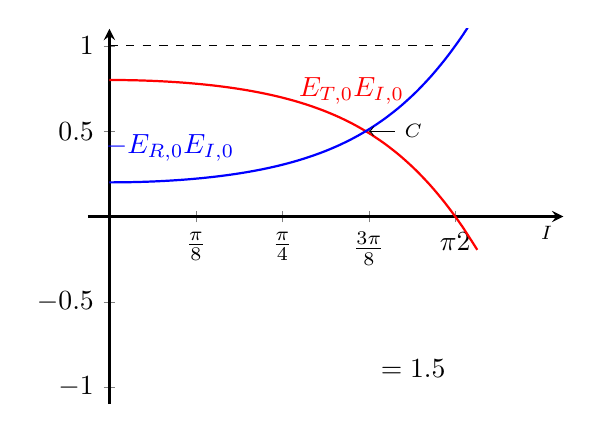
\begin{tikzpicture}
        \pgfmathsetmacro\ben{1.5}
        \pgfmathsetmacro\ls{0.15}
        \begin{axis}[
            standardplot,
            xmin=0, xmax=5, ymin=-1, ymax=1,
            xlabel={$\te_I$},
            domain=0:4,
            range=-1:1,
            xtick={0,1,2,3,4},
            xticklabels={$0$,$\frac{\pi}{8}$,$\frac{\pi}{4}$,$\frac{3\pi}{8}$,$\f{\pi}{2}$},
            ytick={-1,-0.5,0,0.5,1},
            yticklabels={$-1$,$-0.5$,$0$,$0.5$,$1$},
            ylabel={},
        ]
        \addplot[domain=0:pi/2+0.1,smooth,thick,red] ({\x/pi*8}, {(2)/(1 + sqrt(1 - (sin(deg(\x))/\ben)^2)/(cos(deg(\x)))*\ben)});
        \addplot[domain=0:pi/2+0.1,smooth,thick,blue] ({\x/pi*8}, {-(1 - sqrt(1 - (sin(deg(\x))/\ben)^2)/(cos(deg(\x)))*\ben)/(1 + sqrt(1 - (sin(deg(\x))/\ben)^2)/(cos(deg(\x)))*\ben)});
        \draw[dashed] (0,1) -- (4,1);
        \draw[red] (2.8,0.6) node[above]{$\f{\ti E_{T,0}}{\ti E_{I,0}}$};
        \draw[blue] (0.7,0.4) node[]{$-\f{\ti E_{R,0}}{\ti E_{I,0}}$};
        \draw[->] (3 + 2*\ls,0.5) node[right]{$\te_C$} -- (3,0.5);
        \draw (4,-1) node[above left]{$\be = 1.5$};
        \end{axis}
\end{tikzpicture}
\end{center}
It can be seen that (for this $\be$), the reflected wave is always out of phase,
\[ \sgn\br{\Re\bc{\ti E_{R,0}}} = \sgn\br{\f{1 - \al\be}{1 + \al \be}}\Re\bc{\ti E_{I,0}} \]
\[ E_{R,0} = \abs{\br{\f{1 - \al\be}{1 + \al \be}}}E_{I,0} \]
Therefore the plot is flipped about the $E_{0} = 0$ axis.\\

As depicted, it is clear to see that there is no Brewster's angle for this system. Are Brewster's angles absent generally?
\[ 0 = \ti E_{R,0} = \br{\f{1-\al\be}{1+\al\be}} \ti E_{I,0} \]
This requires,
\[ 1 = \al\be = \br{\f{\mu_1 v_1}{\mu_2 v_2}}\br{\f{\cos \te_T}{\cos \te_I}} = \f{\sqrt{1 - \br{n_1/n_2}^2\sin^2 \te_I}}{\cos \te_I}\br{\f{\mu_1 v_1}{\mu_2 v_2}} \]
\[ 1 = \f{1 - \br{v_2/v_1}^2\sin^2 \te_I}{\cos^2 \te_I}\br{\f{\mu_1}{\mu_2}}^2\br{\f{v_1}{v_2}}^2 \]
\[ 1 = - \br{\f{v_2}{v_1}}^2\sin^2 \te_I\f{1}{\cos^2 \te_I}\br{\f{\mu_1}{\mu_2}}^2\br{\f{v_1}{v_2}}^2 +   \f{1}{\cos^2 \te_I}\br{\f{\mu_1}{\mu_2}}^2\br{\f{v_1}{v_2}}^2 \]
\[ 1 = - \sin^2 \te_I\f{1}{\cos^2 \te_I}\br{\f{\mu_1}{\mu_2}}^2+\f{1}{\cos^2 \te_I}\br{\f{\mu_1}{\mu_2}}^2\br{\f{v_1}{v_2}}^2 \]
\[ \cos^2 \te_I \br{\f{\mu_2}{\mu_1}}^2 = -\sin^2 \te_I+\br{\f{v_1}{v_2}}^2 \]
\[ \cos^2 \te_I \br{\f{\mu_2}{\mu_1}}^2 + 1 - \cos^2 \te_I = +\br{\f{v_1}{v_2}}^2 \]
\[ \cos^2 \te_I = \f{\br{\f{v_1}{v_2}}^2 - 1}{\br{\f{\mu_2}{\mu_1}}^2 - 1} \]
Which gives a Brewster's angle of,
\[ \te_B = \arccos\br{\sqrt{\f{\br{{v_1}/{v_2}}^2 - 1}{\br{{\mu_2}/{\mu_1}}^2 - 1}}} \]
In order for $\te_B$ to exist, it must be that
\[ 0 \leq \f{\br{{v_1}/{v_2}}^2 - 1}{\br{{\mu_2}/{\mu_1}}^2 - 1} \leq 1 \]
This requires ${\mu_2}/{\mu_1}$ to be different from $1$. Therefore for materials where ${\mu_2}/{\mu_1} \approx 1$, there is no Brewster angle (unless ${v_2}/{v_1} \approx {\mu_2}/{\mu_1}$). This exotic case corresponds to the case where the two media are optically indistinguishable. Nonetheless, there could easily be a Brewster angle for $\be = 1.5$.\\

At normal incidence, $\te_I = 0$,
\[ \al\br{\te_I} = 1 \]
This reduces the Fresnel equations from \cref{eq:fresnel_perpend} to,
\[ \ti E_{T,0} = \br{\f{2}{1 +  \be}}\ti E_{I,0} \qquad \ti E_{R,0} = \br{\f{1 - \be}{1 +  \be}}\ti E_{I,0}\]

The reflection and transmission coefficients are defined as,
\begin{align*}
    R &= \f{I_R}{I_I} = \br{\f{\ti E_{R,0}}{\ti E_{I,0}}}^2 \\
    T &= \f{I_T}{I_I} = \f{\ep_2 v_2}{\ep_1 v_1}\br{\f{\ti E_{T,0}}{\ti E_{I,0}}}^2 \f{\cos \te_T}{\cos \te_I}
\end{align*}
Explicitly,
\begin{align*}
    R &= \br{\f{1 - \al\be}{1 + \al\be}}^2 \\
    T &= \be\br{\f{2}{1+\al\be}}^2 \al
\end{align*}
Checking that the coefficients sum to $1$,
\begin{align*}
    T + R
    &= \be\br{\f{2}{1+\al\be}}^2 \al + \br{\f{1 - \al\be}{1 + \al\be}}^2 \\
    &= \f{1}{\br{1 + \al\be}^2} \br{4 \al\be + 1 - 2 \al\be + \al^2\be^2} \\
    &= \f{1}{\br{1 + \al\be}^2} \br{1 + 2 \al\be + \al^2\be^2} \\
    &= \f{1}{\br{1 + \al\be}^2} \br{1 + \al\be}^2 \\
    &= 1
\end{align*}

\subsection{Frequency Dependence of Permittivity}
Electromagnetic wave propagation depends on $\ep, \mu$ and $\si$ and we have, so far, assumed that these are frequency independent. If we elevate $\mu, \ep$ and $\si$ to depend on $\w$ we have that,
\[ v\br{\w} = \f{1}{\sqrt{\mu\br{\w} \ep \br{\w}}} \]
This phenomena is know as \term{dispersion}. The index of refraction is modified also,
\[ n \br{\w} = \f{c}{v\br{\w}} \]
Any wave packet will have a \term{phase velocity} (the speed of the surfaces of constant phase),
\[ v = \f{\w}{k} = f \la \]
While the \term{group velocity} is the speed of the wave packet.
\[ v_g = \der{\w}{k} = \f{\dif E / \dif k}{\dif E / \dif \w} \]
We will learn that $v v_g = c^2$ always.\\

In order to get a mathematical model for this, let's look at the 1D, damped, driven, harmonic oscillator.
\[ m \ddot {\ti x} = - m\w_0^2 {\ti x} - m \ga \dot {\ti x} + F_0 e^{i \w t} \]
Where $m \ga \dot {\ti x}$ and $F_0 e^{i \w t}$ is a driven force. This equation motivates the ansatz,
\[ x\br{t} = \Re\br{\ti x_0 e^{i\w t}} \]
Which induces the auxiliary equation,
\[ - \w^2 \ti x_0 - i \ga \w \ti x_0 + \w_0^2 \ti x_0 = \f{F_0}{m} \]
Rearranging,
\[ \ti x_0 = \f{F_0}{m} \f{1}{\w_0^2 - \w^2 - i \ga \w} = \f{F_0}{m} \f{\br{\w_0^2 - \w^2} + i \ga \w}{\br{\w_0^2 - \w^2} + \br{\ga \w}^2} = x_0 e^{i \de} \]
If $\ti{F}\br{t} = w E_0 e^{i \w t}$ then the dipole moment of the oscillator will be the real part of $\ti p \br{t} = \w \ti x \br{t}$ where $\ti p \br{t}$ is,
\[ \ti p \br{t} = \f{q^2 E_0 e^{i \w t}}{m} \f{1}{\w_0^2 - \w^2 - i \ga \w} = \f{q^2 E_0 e^{i \w t}}{m} \f{\br{\w_0^2 - \w^2} + i \ga \w}{\br{\w_0^2 - \w^2} + \br{\ga \w}^2} \]
So that $\ti p \br{t}$ an $\ti E\br{t}$ will have a phase difference,
\[ \de = \tan^{-1} \br{\f{\ga \w}{\w_0^2 - \w^2}} \]
So that the phase difference itself is frequency dependent. \\

We now have the result for a damped, driven, harmonic oscillator and found the  polarization to be,
\[ \ti{p}\br{t} = \f{q^2 E_0 e^{-i\w t}}{\ep_0 m} \f{1}{\w_0^2 - \w^2 - i \ga \w} \]
This result holds for a single oscillator with natural frequency $\w_0$ and damping $\ga$ ($\w$ is the frequency of the driving force and $\w_0$ is the natural frequency).\\

For polarizable media we have many oscillators and we can write the polarization density as,
\[ \ti{\ve P}\br{\w} = \f{N q^2}{\ep_0 m} \bc{\sum_{j} \f{f_j}{\w_j^2 - \w^2 - i \ga_j \w}} \ti{\ve E}\br{\w} \]
Recall that $\ve E = \ve D - \ve P$ and $\ve E = \ep \ve D, \ve P = \ep_0 \chi \ve E$. Where the susceptibility is,
\[ \chi = \f{N q^2}{\ep_0 m} \bc{\sum_{j} \f{f_j}{\w_j^2 - \w^2 - i \ga_j \w}} \]
Previously, this was taken to be a constant but now it is frequency dependent $\chi \mapsto \chi\br{\w}$. It is convenient to introduce the complex dielectric constant,
\[ \ti \ep = \ep_0 \br{1 + \ti \chi} \]
We make the approximation that $\ti \chi$ is reasonably small such that we can make the approximation,
\[ \sqrt{\ti \ep} \approx \sqrt{\ep} \br{1 + \f12 \ti \chi} \]
And the wave equation can be rewritten as,
\[ \del^2 \ti{\ve E} = \ti \ep \mu_0 \pdder{\ti{\ve E}}{t} \]
With solution,
\[ \ti{\ve E}\br{z, t} = \ti{\ve E}_0 e^{i\br{\ti k z - \w t}} = \ti{\ve E}_0 e^{- \Im\br{\ti k} z} e^{i\br{\Re\br{\ti k} z - \w t}} \]
Where,
\[ \ti k = \w \sqrt{\ti \ep \mu_0} = \f{\w \sqrt{\ti \ep \mu_0}}{c \sqrt{\ep \mu_0}} = \f{\w}{c}\br{1 + \f{N q^2}{2 m \ep_0} \sum_j \f{f_j}{\w_j^2 - \w^2 - i \ga_j \w}} \]
And the refractive index is,
\[ n = \f{c}{v} = \f{ck}{\w} = \f{c}{\w} \Re\br{\ti k} \]
\[ n \approx 1 + \f{N q^2}{2 m \ep_0} \sum_j \f{f_j\br{\w_0^2 - \w^2}}{\br{\w_j^2 - \w^2}^2 + \br{\ga_j \w}^2} \]
We make a distinction: \term{Normal Dispersion} occurs when $\dif n / \dif \la > 0$ while \term{Anomalous Dispersion} occurs when $\dif n / \dif \la < 0$. (do not get confused here; $n = \f{c}{v} = \f{c}{\la f} = \f{c k}{\w}$ holds for always)\\
While the absorption coefficient is $\al = 2 \Im\br{\ti k}$,
\[ \al \approx \f{N q^2 \w^2 }{m c \ep_0} \sum_j \f{f_j \ga_j}{\br{\w_j^2 - \w^2}^2 + \br{\ga_j \w}^2} \]
\subsection{Plasma Frequency}
In the high frequency limit we can expand the sum.
\[ \ti k \sqrt{\ti \ep \mu_0} \w = \f{\w}{c} \sqrt{\ti \ep} = \f{\w}{c} \br{1 + \f{N q^2}{m} \sum_j \f{f_j}{\w_j^2 - \w^2 - i \ga_j \w}} \approx \f{\w}{c}\br{1 - \f{NZ q^2}{m \w^2}} \]
Where $Z = \sum_j f_j$ is the number of electrons per unit volume. This can be wrtitten as $\ti n = \f{c \ti k}{\w} = 1 - \f{\w_p^2}{\w^2}$ where,
\[ \w_p^2 = \f{Nq^2 Z}{m} \]
Is the \term{plasma frequency}.

\subsection{Guided Waves}

A \term{waveguide} is a tube in which a good conductor is evenly spread across the inner walls. It will be our working setting that the wave guide is oriented along the $z$-axis. A \textit{good} waveguide is one where the walls wrap entirely around the central axis and is very long such that there are no fringing effects to consider. In particular, waveguides are designed with specific wavelengths in mind so that these waves are resonant with the waveguide, guiding it down its axis. \\

Along the waveguide there will typically be a traveling wave component $e^{i\br{kx - \w t}}$ and a transverse component with a functional dependence on $x ,y$. The boundary conditions for a waveguide are,
\[ \hat n \times \ve E \mid\tsb{inner walls} = \ve 0 \]
\[ \hat n \cdot \ve B \mid\tsb{inner walls} = 0 \]
Where $\hat n$ is the normal to the walls oriented inward.\\

Recall that for plane waves,
\[ \ti {\ve E}\br{\ve r, t} = \ti {\ve E}_0 e^{i\br{\ve k \cdot \vr r - \w t}}\]
In waveguides we no longer have plane waves. The waves will be traveling in the $z$ direction with $x,y$ dependence. Now we have,
\[ \ti {\ve E}\br{\ve r, t} = \ti {\ve E}_0 e^{i\br{k_z z - \w t}}\]
Where $\ti {\ve E}_0$ has functional dependence,
\[ \ti {\ve E}_0 = \ti {\ve E}_0\br{x,y} = \ti {\ve E}_0\br{r, \phi} \]
Where $r, \phi$ are the polar coordinates. The same holds for the $\ve B$ field as well. Note that $\ti {\ve E}_0$'s doesn't depend on $z$ but certainly can have a $\hat z$ component.
\[ \pder{}{z}\ti {\ve E}_0 = 0 \qquad \ti {\ve E}_0 \cdot \hat z = {\ti E}_{0z}\]
So that,
\[ \ti {\ve E}_0 = \ti {E}_{0x} \br{x,y} \hat x + \ti {E}_{0y} \br{x,y} \hat y + \ti {E}_{0z} \br{x,y} \hat z \]
Naturally the wave equation takes on a different form in a waveguide. We introduce the \term{transverse vector differential},
\[ \vdel_{\perp} = \vdel - \hat z \pder{}{z} \]
Which can be written in different coordinates,
\[ \vdel_{\perp} = \hat x \pder{}{x} + \hat y \pder{}{y} = \hat s \pder{}{s} + \hat \phi \f{1}{s} \pder{}{\phi} \]
The \term{transverse Laplacian} is,
\[ \del_{\perp}^2 = \del^2 - \pdder{}{z} \]
Generally, the wave equation takes the form,
\[ \br{\del^2 - \mu \ep \pdder{}{t}} \ti {\ve E} = 0 \]
This becomes,
\[ \br{\del_{\perp}^2 + \pdder{}{z} - \mu \ep \pdder{}{t}} \ti {\ve E} = 0 \]
With for the traveling wave solution is really,
\[ \br{\del_{\perp}^2 - k_z^2 + \mu \ep \w^2} \ti {\ve E} = 0 \eq \label{eq:wave_guide_E}\]
Similarly,
\[ \br{\del_{\perp}^2 - k_z^2 + \mu \ep \w^2} \ti {\ve B} = 0 \eq \label{eq:wave_guide_B}\]
It is often useful to use the following notation,
\[ \ti {\ve E} = \hat z \ti {E}_z + \br{\hat z \times \ti {\ve E}} \times z = \ti {\ve E}_z + \ti {\ve E}_{\perp} \]

To solve waveguide problems, we need to solve \cref{eq:wave_guide_E,eq:wave_guide_B}.
\[ \ti {\ve E}\br{\ve r, t} = \ti {\ve E}_0\br{x,y} e^{i\br{k_z z - \w t}}\]
Explicitly,
\[ \vdel \times \ti {\ve E} = - \pder{\ti {\ve B}}{t} = i \w \ti {\ve B} \implies \hat z \cdot \vdel_{\perp} \times \ti {\ve E}_{\perp} = i \w \ti B_z \]
Where $\br{\vdel \times \ti {\ve E}}$ has $z$ component,
\begin{align*}
\hat z \times \br{\vdel \times \ti {\ve E}}
&= i \w \hat z \times \br{\hat z \ti B_z + \ti{\ve B}_{\perp}}\\
&= i \w \hat z \times \ti{\ve B}_{\perp}\\
&= \br{\pder{\ti E_z}{y} - \pder{\ti E_y}{z}} \hat y - \br{\pder{\ti E_x}{z} - \pder{\ti E_z}{x}} \hat x \\
&= \br{\hat y \pder{}{y} + \hat x \pder{}{x}} \ti E_z - \pder{}{z}\br{\ti E_y \hat y + \ti E_x \hat x} \qquad \text{Collect terms}\\
&= \vdel_{\perp} \ti E_z - i k_z \ti {\ve E}_{\perp}
\end{align*}
There we have the following wave equation,
\[ i \w \hat z \times \ti{\ve B}_{\perp} + i k_z \ti {\ve E}_{\perp} = \vdel_{\perp} \ti E_z \]
Analogously for Faraday's equation we have the following,
\[ \vdel \times \ti {\ve B} = \mu_0 \ep_0 \pder{\ti {\ve E}}{t} \]
Which, after similar algebra yields,
\[ i \w \mu_0 \ep_0 \hat z \times \ti{\ve E}_{\perp} + i k_z \ti {\ve B}_{\perp} = \vdel_{\perp} \ti B_z \]
The remaining of Maxwell's equations can be written for waveguides,
\[ \vdel \cdot \ti {\ve E} = 0 \implies \vdel_{\perp} \cdot \ti{\ve E}_{\perp} = -i k_z \ti E_z \]
\[ \vdel \cdot \ti {\ve B} = 0 \implies \vdel_{\perp} \cdot \ti{\ve B}_{\perp} = -i k_z \ti B_z \]

Altogether we have \term{Maxwell's equations for waveguides}:
\begin{align*}
    \eq \label{eq:wave_guide_me}
    \begin{split}
    \vdel_{\perp} \cdot \ti{\ve E}_{\perp} &= -i k_z \ti E_z \\
    \vdel_{\perp} \cdot \ti{\ve B}_{\perp} &= -i k_z \ti B_z \\
    i \w \hat z \times \ti{\ve B}_{\perp} + i k_z \ti {\ve E}_{\perp} &= \vdel_{\perp} \ti E_z \\
    i \w \mu_0 \ep_0 \hat z \times \ti{\ve E}_{\perp} + i k_z \ti {\ve B}_{\perp} &= \vdel_{\perp} \ti B_z \\
    \vdel_{\perp} \times \ti {\ve E}_{\perp} &= i \w \ti {\ve B}_z
    \end{split}
\end{align*}

\subsubsection{Transverse Electric and Magnetic (TEM) waves}

Transverse electric and magnetic waves are those where $\ti E_z = \ti B_z = 0$. However through substitution into \cref{eq:wave_guide_me}, one arrives at $\vdel \times \ve E = 0$ which enforces that $\del^2 V = 0$ holds true in the waveguide. Since $\del^2 V$ has no local extrema away from the sides of the waveguide, this implies that hollow metal tubes don't emit EM radiation! This is obviously wrong so our assumption that the waves were transverse must be mistaken. Therefore either $\ti E_z$ or $\te B_z$ or both must be \textit{non-zero}. In fact, rectangular, circular, elliptical (any shaped hollow, metallic waveguides) \textbf{cannot} support TEM waves. Nonetheless, it can be shown that at least two separate conductors are required for TEM waves to exist. \\

To illustrate this concretely, consider the case of a coaxial cable as a waveguide. The transverse components are exactly as was found for a DC system:
\[ \ve E_{0}\br{s, \phi} = \hat s \f{V_0}{s \ln \br{\f{b}{a}}} \qquad \ve B_{0}\br{s, \phi} = \hat \phi \f{\mu I}{2 \pi s} \]
Which admits no longitudinal components!\\

To illustrate the TEM problem more clearly, it is possible to connect the transverse and longitudinal components directly together. Upon examination of \cref{eq:wave_guide_me}, it is possible to take,
\[ \w \hat z \times \ti{\ve B}_{\perp} + i k_z \ti {\ve E}_{\perp} = \vdel_{\perp} \ti E_z \]
And substitute for $\ti{\ve B}_{\perp}$ from
\[ i \w \mu \ep \hat z \times \ti{\ve E}_{\perp} + i k_z \ti {\ve B}_{\perp} = \vdel_{\perp} \ti B_z \]
To get,
\[ \f{\w}{i k_z} \hat z \times \bc{\vdel_{\perp} \ti B_z - i \w \mu \ep \hat z \times \ti{\ve E}_{\perp}} + i k_z \ti {\ve E}_{\perp} = \vdel_{\perp} \ti E_z \]
\[ \f{\w}{i k_z} \hat z \times \vdel_{\perp} \ti B_z + i k_z \ti {\ve E}_{\perp} = \vdel_{\perp} \ti E_z \]
Which yields the followings equations,
\[ \ti {\ve E}_{\perp} = \f{i}{\mu \ep \w^2 - k_z^2} \br{k_z \vdel_{\perp} \ti E_{z} - \w \hat z \times \vdel_{\perp} \ti B_z} \eq \label{eq:long_from_trans_1} \]
And similarly one can derive,
\[ \ti {\ve B}_{\perp} = \f{i}{\mu \ep \w^2 - k_z^2} \br{k_z \vdel_{\perp} \ti B_{z} - \mu \ep \w \hat z \times \vdel_{\perp} \ti E_z} \eq \label{eq:long_from_trans_2} \]
Which means that if we know the longitudinal parts $\ti E_z$ or $\ti B_z$, then we can easily find the transverse parts $\ti {\ve E}_{\perp}$ and $\ti {\ve E}_{\perp}$. \\

Note that for TEM waves, $k^2 = \mu \ep \w^2$ and so the equations above are not valid. In order to study the cases of transverse electric and transverse magnetic waves, let us consider a rectangular waveguide with width $a$ and height $b$.

\subsubsection{Transverse Electric (TE) waves}
In a rectangular wave guide, the following boundary conditions for TE waves are imposed by Maxwell's equations,
\begin{align*}
    \ve E^{\parallel} &= \ve 0 \\
    B^{\perp} &= 0
\end{align*}
Treating the waveguide as a tube oriented in the $z > 0$ direction, a generic monochromatic wave has form,
\begin{align*}
    \ti{\ve E}\br{x, y, z, t} &= \ti{\ve E}_0 \br{x, y} e^{i\br{k z - \w t}} \eq \label{eq:TM}\\
    \ti{\ve B}\br{x, y, z, t} &= \ti{\ve B}_0 \br{x, y} e^{i\br{k z - \w t}} \eq \label{eq:TE}
\end{align*}
Maxwell's equations enforce the following system of constraints,
\begin{align*}
\eq \label{eq:main_waveguide_eqn}
\begin{split}
    E_x &= \f{i}{\br{\w / c}^2 - k^2} \br{k \pder{E_z}{x} + \w \pder{B_z}{y}} \\
    E_y &= \f{i}{\br{\w / c}^2 - k^2} \br{k \pder{E_z}{y} - \w \pder{B_z}{x}} \\
    B_x &= \f{i}{\br{\w / c}^2 - k^2} \br{k \pder{B_z}{x} - \f{\w}{c^2} \pder{E_z}{y}} \\
    B_y &= \f{i}{\br{\w / c}^2 - k^2} \br{k \pder{B_z}{y} + \f{\w}{c^2} \pder{E_z}{x}}
\end{split}
\end{align*}
Whose second derivatives reduce the system to,
\begin{align*}
    \bs{\pdder{}{x} + \pdder{}{y} + \br{\f \w c}^2 - k^2} E_z &= 0 \eq \label{eq:Ez}\\
    \bs{\pdder{}{x} + \pdder{}{y} + \br{\f \w c}^2 + k^2} B_z &= 0 \eq \label{eq:Bz}
\end{align*}
Since \cref{eq:long_from_trans_1,eq:long_from_trans_2} can be used to calculate the longitudinal components, the Poynting vector is entirely determined. Explicitly its time-averaged value can be calculated directly using a trick,
\[ \ba{\ve S} = \f{1}{\mu_0} \ba{\ve E \times \ve B} = \f{1}{2 \mu_0} \Re\br{\ti{\ve E} \times \ti{\ve B}^*} \]
For a rectangular waveguide, $B_z$ becomes a standing wave quantized by the boundary conditions. Separation of variables for the $x$ and $y$ components gives the following,
\[ B_z = B_0 \cos \br{\f{m \pi x}{a}} \cos \br{\f{n \pi y}{b}} \quad m, n = 0, 1, 2,\ldots \]
This result in conjunction with the above system of equations (\cref{eq:main_waveguide_eqn}) fixes the $x,y$ components of both $\ve E$ and $\ve B$. For ease of notation let,
\[ \text{cc}_{mn}\br{x,y} = \cos \br{\f{m \pi x}{a}} \cos \br{\f{n \pi y}{b}} \]
Compactly written,
\begin{align*}
    E_z &= 0 \\
    E_y &= \f{-i \w}{\br{\w / c}^2 - k^2} \br{- \f{m \pi}{a}} B_0 \text{sc}_{mn} \\
    E_x &= \f{i \w}{\br{\w / c}^2 - k^2} \br{- \f{n \pi}{b}} B_0 \text{cs}_{mn} \\
    B_x &= \f{i k}{\br{\w / c}^2 - k^2} \br{- \f{m \pi}{a}} B_0 \text{sc}_{mn} \\
    B_y &= \f{i k}{\br{\w / c}^2 - k^2} \br{- \f{n \pi}{b}} B_0 \text{cs}_{mn} \\
    B_z &= B_0 \text{cc}_{mn}
\end{align*}
Therefore,
\begin{align*}
\br{\ti{\ve E} \times \ti{\ve B}^*} \cdot \hat x
&= \ti{E}_y\ti{B}_z^* - \ti{E}_z\ti{B}_y^* \\
&= \ti{E}_y\ti{B}_z^* \\
&= \ti{E}_{0, y}\ti{B}_{0, z}^* e^{i \br{k z - \w t}}e^{-i \br{k z - \w t}} \\
&= \ti{E}_{0, y}\ti{B}_{0, z}^* \\
&= \f{-i \w}{\br{\w / c}^2 - k^2} \br{- \f{m \pi}{a}} B_0 \text{sc}_{mn} B_0 \text{cc}_{mn}
\end{align*}
Similarly for $y$,
\[ \br{\ti{\ve E} \times \ti{\ve B}^*} \cdot \hat y = - \f{i \w}{\br{\w / c}^2 - k^2} \br{- \f{n \pi}{b}} B_0 \text{cs}_{mn} B_0 \text{cc}_{mn}\]
While $z$ is different,
\begin{align*}
\br{\ti{\ve E} \times \ti{\ve B}^*} \cdot \hat z
&= \ti{E}_x\ti{B}_y^* - \ti{E}_y\ti{B}_x^* \\
&= \ti{E}_{0,x}\ti{B}_{0,y}^* - \ti{E}_{0,y}\ti{B}_{0,x}^* \\
&= \f{i \w}{\br{\w / c}^2 - k^2} \br{- \f{n \pi}{b}} B_0 \text{cs}_{mn} \f{\br{-i} k}{\br{\w / c}^2 - k^2} \br{- \f{n \pi}{b}} B_0 \text{cs}_{mn} \\ &\quad- \f{-i \w}{\br{\w / c}^2 - k^2} \br{- \f{m \pi}{a}} B_0 \text{sc}_{mn} \f{\br{-i} k}{\br{\w / c}^2 - k^2} \br{- \f{m \pi}{a}} B_0 \text{sc}_{mn}
\end{align*}
Therefore there are components of $\ba{\ve S}$ in all directions. The only component that is relevant for the cross-sectional area of the waveguide is the $\hat z$ component. Therefore cleaning up the previous result,
\[ \br{\ti{\ve E} \times \ti{\ve B}^*} \cdot \hat z = \f{i \w}{\br{\w / c}^2 - k^2} \br{\f{n \pi}{b}}^2 B_0^2 \text{cs}^2_{mn} \f{-i k}{\br{\w / c}^2 - k^2} - \f{-i \w}{\br{\w / c}^2 - k^2} \br{\f{m \pi}{a}}^2 B_0^2 \text{sc}^2_{mn} \f{-i k}{\br{\w / c}^2 - k^2} \]
\[ \br{\ti{\ve E} \times \ti{\ve B}^*} \cdot \hat z = \w k\bs{\br{\w / c}^2 - k^2}^{-2} B_0^2 \bc{\br{\f{n \pi}{b}}^2  \text{cs}^2_{mn} + \br{\f{m \pi}{a}}^2 \text{sc}^2_{mn}} \]
Therefore,
\[ \ba{\ve S} \cdot \hat z = \f{1}{2\mu_0}\w k\bs{\br{\w / c}^2 - k^2}^{-2} B_0^2 \bc{\br{\f{n \pi}{b}}^2  \text{cs}^2_{mn} + \br{\f{m \pi}{a}}^2 \text{sc}^2_{mn}} \]
Make use of the following shorthand,
\[ \w_{mn} = c \pi \sqrt{\br{m/a}^2 + \br{n/b}^2} \]
And,
\[ k = c^{-1} \sqrt{\w^2 - \w_{mn}^2} \]
Cleans up the notation,
\[ \ba{\ve S} \cdot \hat z = \f{\pi^2 \w k}{2\mu_0} \f{c^4}{\w_{mn}^4} B_0^2 \bc{\br{\f{n}{b}}^2  \text{cs}^2_{mn} + \br{\f{m}{a}}^2 \text{sc}^2_{mn}} \]
Integrating across the entire cross section of the tube amounts to calculating,
\[ \int_{0}^{a} \dif x \int_{0}^{b} \dif y \br{\br{\f{n}{b}}^2  \text{cs}^2_{mn} + \br{\f{m}{a}}^2 \text{sc}^2_{mn}} = \f{ab}{4}\br{\br{\f{n}{b}}^2 + \br{\f{m}{a}}^2} \eq \label{eq:area_sum}\]
Therefore,
\[ \int_{\s{A}} \ba{\ve S} \cdot \dif \ve a = \f{\pi^2 \w k}{2\mu_0} \f{c^4}{\w_{mn}^4} B_0^2 \f{ab}{4}\br{\br{\f{n}{b}}^2 + \br{\f{m}{a}}^2} \]
\[ \int_{\s{A}} \ba{\ve S} \cdot \dif \ve a = \f{\w k}{2\mu_0} \f{c^2}{\w_{mn}^2} B_0^2 \f{ab}{4} \]
Analogous we have the total energy density averaged over time,
\begin{align*}
    \ba{u}
    &= \f14 \Re\br{\ep_0 \ti{\ve E} \cdot \ti{\ve E}^* + \f{1}{\mu_0} \ti{\ve B} \cdot \ti{\ve B}^*} \\
    &= \f14 \Re\br{\ep_0 \ti{\ve E}_0 \cdot \ti{\ve E}_0^* + \f{1}{\mu_0} \ti{\ve B}_0 \cdot \ti{\ve B}_0^*} \\
    &= \f14 \Re\br{\ep_0 \br{\br{\f{\w}{\br{\w / c}^2 - k^2} \br{- \f{n \pi}{b}} B_0 \text{cs}_{mn}}^2  + \br{\f{-\w}{\br{\w / c}^2 - k^2} \br{- \f{m \pi}{a}} B_0 \text{sc}_{mn}}}^2 + \f{1}{\mu_0} \ti{\ve B}_0 \cdot \ti{\ve B}_0^*} \\
    &= \f14 \Re\br{\ep_0 B_0^2\w^2 \bs{\br{\w / c}^2 - k^2}^{-2}\br{\br{\f{n \pi}{b}}^2 \text{cs}^2_{mn} + \br{\f{m \pi}{a}}^2 \text{sc}^2_{mn}} + \f{1}{\mu_0} \ti{\ve B}_0 \cdot \ti{\ve B}_0^*} \\
    &= \f14 \Re\br{\ep_0 B_0^2\w^2 \pi^2 \f{c^4}{\w_{mn}^4}\br{\br{\f{n}{b}}^2 \text{cs}^2_{mn} + \br{\f{m}{a}}^2 \text{sc}^2_{mn}} + \f{1}{\mu_0} \ti{\ve B}_0 \cdot \ti{\ve B}_0^*} \\
    &= \f14 \bigg\{\ep_0 B_0^2\w^2 \pi^2 \f{c^4}{\w_{mn}^4}\br{\br{\f{n}{b}}^2 \text{cs}^2_{mn} + \br{\f{m}{a}}^2 \text{sc}^2_{mn}}  + \\
    &= + \f{1}{\mu_0} B_0^2 \text{cc}^2_{mn} + \f{k^2 \pi^2 B_0^2}{\mu_0} \f{c^4}{\w_{mn}^4} \br{\br{\f{n}{b}}^2 \text{cs}^2_{mn} + \br{\f{m}{a}}^2 \text{sc}^2_{mn}} \bigg\}
\end{align*}
Making use of \cref{eq:area_sum} again,
\[ \int_{\s{A}} \ba{u} \dif a = \f{1}{2 \mu_0} \f{ab}{4}\f{\w^2}{\w^2_{mn}} B_0^2\]
Therefore,
\[ \f{\int_{\s{A}} \ba{\ve S} \cdot \dif \ve a}{\int_{\s{A}} \ba{u} \dif a} = \f{k c^2}{\w} = \f{c^2}{\w}\sqrt{\w^2 - \w_{mn}^2} = v_g \]

\subsubsection{Transverse Electric (TM) waves}
In the previous section, we worked out the form for TE waves in a rectangular waveguide. This was directly motivated by trying to match the boundary condition \cref{eq:TE} in the restricted case of TE waves where $E_z = 0$. Instead, we can restrict the focus to TM waves where $B_z = 0$. In this case we need to focus on the boundary condition \cref{eq:TE}. Assume that $E_z\br{x,y}$ is separable,
\[ E_z\br{x,y} = X\br{x}Y\br{y} \]
And attempt to solve \cref{eq:Ez}.
\[ \bs{\pdder{}{x} + \pdder{}{y} + \br{\f \w c}^2 - k^2} E_z = 0 \]
\[ \bs{\pdder{}{x} + \pdder{}{y} + \br{\f \w c}^2 - k^2} XY = 0 \]
\[ Y\pdder{}{x}X + X\pdder{}{y}Y + \br{\f \w c}^2 XY - k^2XY = 0 \]
\[ \f{1}{X}\pdder{X}{x} + \f{1}{Y}\pdder{Y}{y} = k^2 - \br{\f \w c}^2  \]
Set separation constants,
\[ \f{1}{X}\pdder{X}{x} = k_x^2 \implies X = X_s \sin\br{k_x x} + X_c \cos\br{k_x x}  \]
But if $E_z = 0$ at the boundaries (\cref{eq:TM}) then we need $X_c$ to vanish and for $\sin\br{k_x x} \to 0$ when $x \to a$. Therefore,
\[ X = X_s \sin\br{\f{m \pi}{a} x} \quad m = 1,2,\ldots\]
The key difference being that $m > 0$ for TM waves; otherwise $E_z = 0$ and we arrive at the trivial solution. Overall we have,
\[ E_z = E_0\sin\br{\f{m \pi}{a} x}\sin\br{\f{n \pi}{b} y} \quad n,m = 1,2,\ldots\]
Plugging this back into \cref{eq:Ez} gives,
\[ -k_x^2 -k_y^2 + \br{\f \w c}^2 - k^2 = 0 \]
\[ -\pi^2\br{\f{m}{a}}^2 -\pi^2\br{\f{n}{b}}^2 + \br{\f \w c}^2 - k^2 = 0 \]
\[ k = \sqrt{\br{\f{\w}{c}}^2 -\pi^2\br{\f{m}{a}}^2 -\pi^2\br{\f{n}{b}}^2 } \]
Maintaining that $k$ be real introduces the cutoff frequency for $\w > \w_{mn}$ where,
\[ \w_{mn} = c \pi \sqrt{\br{\f{m}{a}}^2 + \br{\f{n}{b}}^2}  \]
Making the wave number,
\[ k = \f{1}{c}\sqrt{\w^2 - \w_{mn}^2} \eq \label{eq:k}\]
And thus fixing the wave velocity,
\[ v = \f{\w}{k}= \f{c}{\sqrt{1 - {\w^2_{mn}}/{\w^2}}} > c \]
Luckily the group velocity is less that the speed of light,
\[ v_g = \der{\w}{k} \]
Which can be obtained from \cref{eq:k},
\[ c^2 k^2 = \w^2 - \w_{mn}^2 \]
Differentiating,
\[ 2 c^2 k \dif k = 2 \w \dif \w \]
Therefore,
\[ v_g = \f{c^2 k}{\w} = \f{c}{\w}\sqrt{\w^2 - \w_{mn}^2} \]
Which is identical for that of TE waves.\\

Since $n,m$ are bounded below by $1$ and not $0$, we have the lowest TM cutoff frequency as the $n, m = 1, 1$ frequency,
\[ \w_{11} = c \pi \sqrt{a^{-2} + b^{-2}} \]
Which is very different from the TE cutoff frequency of $\w_{10}$,
\[ \f{\w_{11}}{\w_{10}} = \f{c \pi \sqrt{a^{-2} + b^{-2}}}{c \pi \sqrt{a^{-2}}} = \sqrt{1 + \br{\f{a}{b}}^2} \]

\subsubsection{TE and TM waves together}
Last time we were examining TE and TM waves and found that the transverse part, $\ti{\ve E}_{\perp}$, was the same as for the DC system we investigated earlier and the longitudinal part $\hat z \ti{B}_z$, was a traveling wave. The boundary conditions led us to the ansatz,
\[ \ti{\ve E}\br{\ve r, t} = \hat y E_0 \sin\br{k_x x} e^{i\br{k_z z - \w t}} \eq \label{eq:rect_waveguide_ansatz}\]
For a traveling wave in a rectangular waveguide we substitute \cref{eq:rect_waveguide_ansatz} into Maxwell's equations,
\[ \vdel \cdot \ve E = \pder{}{y}E_y = 0 \]
Which is satisfied by \cref{eq:rect_waveguide_ansatz}. Next we would like to check this ansatz against $\vdel \times \ve E = - \pder{\ve B}{t}$ but this can get messy. Instead check the wave equation for $\ve E$,
\[ \del^2 \ti{\ve E} - \mu \ep \pdder{\ti{\ve E}}{t} = 0 \]
In Cartesian coordinates,
\[ \br{\pdder{}{x} + \pdder{}{y} + \pdder{}{z} - \mu \ep \pdder{}{t}}\ti{\ve E} = 0 \]
This leading operator is the \term{D'Alembertian operator}\footnote{Sometimes you will see this written as $\Box$ or $\Box^2$. This is reminiscent of special relativity where $\de_\mu = \br{\mu \ep \pder{}{t}, \vdel}$},
\[ \Box^2 = \pdder{}{x} + \pdder{}{y} + \pdder{}{z} - \mu \ep \pdder{}{t} \]
Applying the wave equation we obtain an auxiliary equation.
\[ \Box^2 \ti{\ve E} = \br{- k_x^2 + 0 - k_y^2 + \mu \ep \w^2} \ti{\ve E} = 0 \]
Avoiding the trivial solution, we require that,
But in order to meet the boundary conditions of the rectangular waveguide,
\[ k_x = \f{m \pi}{a} \quad m \in \N \]
So that $k_z$ is fixed as well,
\[ k_z = \sqrt{\mu \ep \w^2 - \br{\f{m \pi}{a}}^2} \]
\[ k_z = \f{\w}{v}\sqrt{1 - \br{\f{m \pi v}{\w a}}^2} \]
Recall that in a vacuum $k_z = \w/ v$. However in the waveguide $k_z$ will be less than $\w / v$. The wavelength is,
\[ \la = \f{2 \pi}{k_z} = \f{2 \pi v}{\w}\br{1 - \br{\f{m \pi v}{\w a}}^2}^{-1/2} \]
Let $\la_0 = 2 \pi v/ \w$ be the vacuum wavelength.
\[ \la = \la_0\br{1 - \br{\f{m \pi v}{\w a}}^2}^{-1/2} \]
Where $\la > \la_0$ is the guide wavelength. And Maxwell's equations for wave guides give,
\begin{align*}
\ti B_z &= B_0 \cos \br{k_x x} \cos\br{k_y y} e^{i\br{k_z z - \w t}} \\
\ti B_x &= \f{-iB_0}{\br{\w/c}^2 - k^2} k k_x \sin \br{k_x x} \cos\br{k_y y} e^{i\br{k_z z - \w t}} \\
\ti B_y &= \f{-iB_0}{\br{\w/c}^2 - k^2} k k_y \cos \br{k_x x} \cos\br{k_y y} e^{i\br{k_z z - \w t}}
\end{align*}
We can also write \cref{eq:rect_waveguide_ansatz} in a different way,
\[ \ti{\ve E}\br{\ve r, t} = \f{1}{2i} E_0 \hat y \br{e^{ik_x x} - e^{-ik_x x}} e^{i \br{k_z z - \w t}} \]
This is nothing more that the sum of two traveling waves,
\[ \ti{\ve E}\br{\ve r, t} = \f{1}{2i} E_0 \hat y \br{e^{i\br{k_x x + k_z z - \w t}} - e^{i\br{-k_x x + k_z z - \w t}}} \]
Where $\ve k_1 = \br{k_x \hat x + k_z \hat z}$ and $\ve k_2 = \br{- k_x x + k_z z}$. These two traveling waves travel down the the cavity in the $\hat z$ direction but are bouncing back and forth off of the boundaries in the $\hat x$ directions.

\section{Potentials \& Fields}
We recall the previously introduced electric, scalar potential $\ve E = - \vdel$ and the magnetic, vector potential $\ve B =\vdel \times\ve A$ because some calculations are easier when using the potentials (which have four components compared to the six components of $\ve E$ and $\ve B$). \\

In electrodynamics we need to reexamine these to see if they are still valid. Regardless we desire that $\vdel \cdot \ve B = 0$ so $\ve B = \vdel \times \ve A$, but we now have Faraday's law:
\[ \vdel \times \ve E = - \pder{}{t} \ve B = -\pder{}{t} \br{\vdel \times \ve A} = - \vdel \times \br{\pder{\ve A}{t}}\]
Rearranging,
\[ \vdel \times \br{\ve E + \pder{\ve A}{t}} = \ve 0 \]
So that the quantity $\ve E + \pder{\ve A}{t}$ becomes the irrotational quantity and so we write,
\[ \ve E + \pder{\ve A}{t} = - \vdel V \]
Which makes the electric potential $\ve E$,
\[ \ve E = - \vdel V - \pder{\ve A}{t} \]
and the $\ve E$ field picks up an extra piece $\pder{\ve A}{t}$. \\

Now let's try these new terms in Gauss's and Ampere's laws:
\[ \ep_0\vdel \cdot \br{-\vdel V + \pder{\ve A}{t}} = \rho \]
So that,
\[ \del^2 V + \pder{}{t}\br{\vdel \cdot \ve A} = -\f{\rho}{\ep_0} \]
Moreover,
\[ \vdel \times \br{\vdel \times \ve A} = \mu_0 \ve J + \mu_0 \ep_0 \pder{}{t} \br{-\vdel V - \pder{\ve A}{t}}\]
\[ \vdel \br{\vdel \cdot \ve A} - \del^2 \ve A = \mu_0 \ve J - \mu_0 \ep_0 \vdel \br{\pder{V}{t}} - \mu_0 \ep_0 \pdder{\ve A}{t} \]
Rearranging this equation gives a familiar form,
\[ \del^2 \ve A - \mu_0 \ep_0 \pdder{\ve A}{t} - \vdel \br{\vdel \cdot \ve A + \mu_0 \ep_0 \pder{V}{t}} = - \mu_0 \ve J \]
Which is precisely the wave-equation for $\ve A$ except for the the ugly term $\vdel\br{\vdel \cdot \ve A + \mu_0 \ep_0 \pder{V}{t}}$. What we will do is \textit{choose} to make this term vanish in order to simplify our system of equations. Therefore we have,
\[ \vdel \cdot \ve A + \mu_0 \ep_0 \pder{V}{t} = 0 \]
Recalling the D'Alembertian operator $\Box^2 = \br{\f{1}{c^2} \pdder{}{t}, \vdel^2}$ we arrive at,
\[ \Box^2 A^{\mu} = -\mu_0 J^{\mu} \]
Where $A^{\mu} = \br{\f{V}{c}, \ve A}$ and $J^{\mu} = \br{c \rho, \ve J}$. In fact if we define $L$ (our generic choice of Gauge) to be,
\[ L = \vdel \cdot \ve A + \mu_0 \ep_0 \pder{V}{t} \]
Then our system becomes,
\begin{align*}
    \Box^2 V + \pder{L}{t} &= - \f{\rho}{\ep_0} \\
    \Box^2 \ve A - \vdel L &= - \mu_0 \ve J
\end{align*}
To show this, one can add zero,
\[ -\f{\rho}{\ep_0} = \del^2 V + \pder{}{t}\br{\vdel \cdot \ve A} + \mu_0 \ep_0 \pdder{V}{t} - \mu_0 \ep_0 \pdder{V}{t}\]
Which allows one to recognize $L$,
\[ -\f{\rho}{\ep_0} = \del^2 V + \pder{}{t}\br{\underbrace{\vdel \cdot \ve A + \mu_0 \ep_0 \pder{V}{t}}_{L}} - \mu_0 \ep_0 \pdder{V}{t}\]
Under the \textit{Lorentz gauge} we set $L = 0$. Therefore,
\[ \Box^2 V = - \f{\rho}{\ep_0} \]
Which means that,
\[ \Box^2 \br{\f{V}{c}} = - \f{c\rho}{\ep_0 c^2} = - \mu_0 \br{c \rho} \]
Which is compactly written in the following form:
\[ \Box^2 A^{\mu} = -\mu_0 J^{\mu} \]
It is also possible to write the gauge $L$ in terms of the 4-potential $A^{\mu}$ and the 4-gradient $\Box = \di_\mu = \br{\f1c\pder{}{t}, \vdel}$,
\[ L = \vdel \cdot \ve A + \f{1}{c^2} \pder{V}{t} = \Box \cdot \br{\f{1}{c} V, \ve A}  = \di_{\mu} A^{\mu} \]
Where the Minkowski metric is $g_{\mu\nu}$ taken to be,
\[ g_{\mu\nu} = g^{\mu\nu} = \begin{pmatrix}
    -1 & 0 & 0 & 0 \\
     0 & 1 & 0 & 0 \\
     0 & 0 & 1 & 0 \\
     0 & 0 & 0 & 1 \\
\end{pmatrix} \]
Such that $\Box^2 = \di^{\mu}\di_{\mu} = g_{\mu\nu} \di^{\mu}\di^{\nu}$.  \\

In general we consider $L$ as a \textit{gauge freedom} because it can be made any value without affecting the $\ve E$ and $\ve B$ fields,
\[ \ve E = - \vdel V - \pder{\ve A}{t} \qquad \ve B = \vdel \times \ve A \]
So far we have seen the \term{Lorentz gauge} (L = 0), but another useful Gauge is the \textit{Coulomb Gauge} where we set $\ve E= - \vdel V$ such that $\del^2 V = - \f{\rho}{\ep_0}$ and thus $\vdel \cdot \ve A = 0$. \\

\subsection{Retarded Potentials}

Consider a density of charge $\rho$ and density of current $\ve J$. The general solution to Maxwell's equations in a static case are,
\[ V\br{\ve r} = \f{1}{4 \pi \ep_0} \int \dif \tau' \f{\rho\br{\ve r'}}{\rcurs} \]
\[ \ve A\br{\ve r} = \f{\mu_0}{4 \pi} \int \dif \tau' \f{\ve J\br{\ve r'}}{\rcurs} \]
Where $\ve r$ is the field point, $\ve r'$ is the source point and $\rcurs = \ve r - \ve r'$ the vector between. However in the dynamic case where $\rho$ and $\ve J$ change quickly with time we have to integrate over at times,
\begin{align*}
V\br{\ve r, t}
&= \f{1}{4 \pi \ep_0} \int \dif \tau' \int \dif t' \de\br{t' - t + \rcurs / c}\f{\rho\br{\ve r', t'}}{\rcurs} \\
&= \f{1}{4 \pi \ep_0} \int \dif \tau'\f{\rho\br{\ve r', t - \rcurs / c}}{\rcurs}
\end{align*}
Intuitively, it takes time for the source at $\ve r'$ to influence points $\ve r$ at a distance of $\rcurs$ away. The influence can only propagate as fast as Maxwell's equations will allow; i.e. the speed of light $c$!\\
Similarly for $\ve A$,
\begin{align*}
\ve A\br{\ve r, t}
&= \f{\mu_0}{4 \pi} \int \dif \tau' \int \dif t' \de\br{t' - t + \rcurs / c}\f{\ve J\br{\ve r', t'}}{\rcurs} \\
&= \f{\mu_0}{4 \pi} \int \dif \tau'\f{\ve J\br{\ve r', t - \rcurs / c}}{\rcurs}
\end{align*}

For both the static and dynamic cases we may write,
\[ A^{\mu} = \br{\f{V}{c}, \ve A} \qquad J^{\mu} = \br{c \rho, \ve J} \]
And Maxwell's equations become,
\[ \Box^2 A^{\mu} = \mu_0 J^{\mu} \]
In the end we get,
\[ \del^2 V - \f{1}{c^2} \pdder{V}{t} = - \f{1}{\ep_0} \rho\br{\ve r, t} \]
And so the retarded potential is a solution to a wave equation we have studied extensively already,
\[ \del^2 V - \mu_0 \ep_0 \pdder{V}{t} = - \f{\rho}{\ep_0} \]

Consider a simple model of a localized source $\rho$ traveling with velocity $\ve v$ such that $\ve J = \rho \ve v$. Without loss of generality, choose $\ve v = v \hat z$ such that,
\[ \ve A \br{\ve r, t} = \f{\mu_0}{4 \pi} \int \dif \tau' \f{\ve J\br{\ve r', t'}}{\rcurs} \]
Where $\ve J\br{\ve r', t'} = \ve J\br{\ve r', t - \rcurs / c}$. For a field point $\ve r$ very far from $\ve r'$, we can claim that $\rcurs \approx r$ and so that,
\[ \ve A \br{\ve r, t} \approx \f{\mu_0}{4 \pi \rcurs} \int \dif \tau' \ve J\br{\ve r', t - r / c} \]
But by the continuity equation $\vdel \cdot \ve J + \di_t \rho = 0$,
\[ \dot \rho \br{t'} = - \vdel \cdot \ve J\br{t'} \]
Recalling that $\ve p$ is the dipole moment,
\[ \ve p = \int \dif \tau \ve r \rho\br{\ve r} \]
We can prove a useful relationship between $\ve p$ and $\ve J$,
\[ \der{\ve p}{t} = \int_{\s V} \dif \tau \ve J\br{\ve r} \]
\textbf{Proof:}
First consider that by definition,
\[ \der{\ve p}{t} = \int_{\s V} \dif \tau \ve r \pder{\rho\br{\ve r, t}}{t} \]
Also product rule yields,
\[ \vdel \cdot \br{\ve r \cdot \ve J} = \ve J + \ve r \vdel \cdot \ve J \]
Therefore,
\[ \intl_{\s V} \dif \tau \vdel \cdot \br{\ve r \cdot \ve J} = \intl_{\di \s V} \dif \ve a \cdot \br{\ve r \cdot \ve J} = \intl_{\s V} \dif \tau \ve J + \intl_{\s V} \dif \tau \ve r \vdel \cdot \ve J \]
Next take $\s V$ to be completely outside all of the sources. Then the surface integral is zero,
\[ 0 = \intl_{\s V} \dif \tau \ve J + \intl_{\s V} \dif \tau \ve r \vdel \cdot \ve J \]
Now apply continuity equation,
\[ \intl_{\s V} \dif \tau \ve J = \intl_{\s V} \dif \tau \ve r \pder{\rho\br{\ve r, t}}{t} = \der{\ve p}{t} \]
Therefore we are able to write,
\[ \dot {\ve p}\br{t'} = \int \dif \tau' \ve J\br{\ve r', t'} \]
Therefore,
\[ \ve A \br{\ve r, t} \approx \f{\mu_0}{4 \pi \rcurs} \dot {\ve p} \br{t - r /c} = \f{\mu_0}{4 \pi \rcurs} \dot {\ve p} \br{-\f{1}{kc}\br{\ve k \cdot \ve r - \w t}} \eq \label{eq:simple_model} \]
A consequence of retarded time due to the speed of light is that $\ve A$ is a traveling wave.

\subsection{Retarded Fields}

For far we have established the concept of retarded time for potentials,
\[ V\br{\ve r, t} = \f{1}{4 \pi \ep_0} \int \dif \tau' \int \dif t' \de\br{t' - t + \rcurs / c}\f{\rho\br{\ve r', t'}}{\rcurs} \]
\[ \ve A\br{\ve r, t} = \f{\mu_0}{4 \pi} \int \dif \tau' \int \dif t' \de\br{t' - t + \rcurs / c}\f{\ve J\br{\ve r', t'}}{\rcurs} \]
Which are simply solutions to Maxwell's equations for potentials. What about fields? Can we write analogously,
\[ \ve E\br{\ve r, t} \stackrel{?}{} \f{1}{4 \pi \ep_0} \int \dif \tau' \int \dif t' \de\br{t' - t + \rcurs / c}\f{\rho\br{\ve r', t'}}{\rcurs^2} \hat \rcurs \]
\[ \ve B\br{\ve r, t} \stackrel{?}{} \f{1}{4 \pi \ep_0} \int \dif \tau' \int \dif t' \de\br{t' - t + \rcurs / c}\f{\ve J\br{\ve r', t'} \times \hat \rcurs}{\rcurs^2}\]
As it turns out, no! These aren't solutions to Maxwell's equations. The simple time delay only works when applied to the potentials that $\ve E$ and $\ve B$ come from. The $\ve E$ and $\ve B$ fields are real in the sense that this is what we measure, whereas the potentials are more fundamental and give us $\ve E$ and $\ve B$ via,
\[ \ve E = - \vdel V - \pder{\ve A}{t} \qquad \ve B = \vdel \times \ve A \eq \label{eq:potential_fields}\]
Or when worked out directly are more complicated,
\[ \ve E \br{\ve r, t} = \f{1}{4 \pi \ep_0} \int \dif \tau' \br{\f{\rho \hat \rcurs}{\rcurs^2} + \f{\dot \rho \hat \rcurs}{c \rcurs} - \f{\dot {\ve J}}{c^2 \rcurs}} \]
\[ \ve B \br{\ve r, t} = \f{\mu_0}{4 \pi} \int \dif \tau' \br{\f{\ve J}{\rcurs^2} + \f{\dot {\ve J}}{c \rcurs}} \times \hat \rcurs \]
Where $\rho = \rho\br{\ve r', t - \rcurs / c}$ and $\ve J = \ve J\br{\ve r', t - \rcurs / c}$ are the time retarded sources. The extra terms are artifacts of carrying out the derivatives in \cref{eq:potential_fields}. These are know as \term{Jefimenko's equations}. It is important to remark about $\vdel \times \ve E = - \di_t \ve B$: we normally sat the changing $\ve B$ field induces an $\ve E$ field which curls. This is a poor choice of words as in reality, the $\ve E$ and $\ve B$ fields are described via the above relations \textit{always} (with or without time dependence). A time changing potential $\ve A$ and $V$ arises from a time changing source $\rho$ and $\ve J$ which results in a time changing $\ve E$ and $\ve B$ which obey Maxwell's equations. They don't induce each other as they are defined separately from the potentials. In conclusion, the potentials are the fundamental things which give us the observable $\ve E$ and $\ve B$ fields.\\

We now return to the simple model of \cref{eq:simple_model},
\[ \ve A \br{\ve r, t} = \f{\mu_0}{4 \pi r} \dot {\ve p}\br{t - r/c} \]
If, for example, we take $\dot {\ve p}$ to be $\dot p \hat z$, then we have,
\[ \ve B = \vdel \times \ve A = \hat x \pder{A_z}{y} - \hat y \pder{A_z}{x} \]
Where,
\[ \pder{A_z}{y} = \pder{r}{y}\pder{A_z}{r} = \f{\mu_0}{4 \pi} \f{y}{r} \br{ - \f{\dot {\ve p}}{r^2} - \f{\ddot {\ve p}}{rc}} = - \f{\mu_0}{4 \pi r^2} \f{y}{r} \br{\dot {\ve p} + \f{r}{c}\ddot {\ve p}} \]
Similarly,
\[ \pder{A_z}{x} = - \f{\mu_0}{4 \pi r^2} \f{x}{r} \br{\dot {\ve p} + \f{r}{c}\ddot {\ve p}} \]
So that,
\[ \ve B \br{\ve r, t} = \f{\mu_0}{4 \pi r^2} \br{\dot {\ve p}\br{t'} + \f{r}{c} \ddot {\ve p}\br{t'}} \times \hat r \eq \label{eq:B_retard}\]
Since the $\dot {\ve p}$ term tends as $1/r^2$ it dominates in the near field approximation and the $\ddot {\ve p}$ terms tends as $1 /r$ and thus dominates far away in the far field approximation. Therefore we consider $\ddot {\ve p}$ to be the \textit{radiation} term.\\

In fact, an antenna with oscillating charge will have changing $\ve E$ and $\ve B$ fields that have strength decreasing as $1/r$. \\

For $t' = r - r/c$,
\[ \der{}{t}\ve p \br{t'} = \cancelto{1}{\der{t'}{t}}\der{}{t'}\ve p \br{t'} = \dot {\ve p}\br{t'}  \]
But the spatial dependence is,
\[ \pder{}{t} \dot {\ve p}\br{t'} = \pder{t'}{r} \pder{}{t'} \dot {\ve p}\br{t'} = - \f{1}{c} \ddot {\ve p}\br{t'} \]
Therefore if we assume that,
\[ \ve p \br{t'} = p_0 \hat z \sin \br{\w t'} = p_0 \hat z \sin \br{\w t - \f{\w}{c} r} \]
And apply \cref{eq:B_retard}, we have that $\ve B$ must point in the $\hat \phi$ direction in cylindrical coordinates. As we have discussed, the radiation term is $ \propto \ddot p / r$. Performing a Taylor series about $t = 0$,
\[ \dot {\ve p}\br{t'} = \dot {\ve p}\br{t - \f{r}{c}} \approx \dot {\ve p}\br{t} - \f{r}{c}\ddot {\ve p}\br{t} + \f{r^2}{2 c^2} \dddot {\ve p}\br{t} + \cdots \]
We have \cref{eq:B_retard} become,
\[ \ve B \br{\ve r, t} = \f{\mu_0}{4 \pi r^2} \br{\dot {\ve p}\br{t} - \f{r^2}{2c^2} \dddot {\ve p}\br{t}}\times \hat r \]
Which means that the non-retarded result is, in this approximation, accurate to second order. \\

Recalling the Jefimenko equations,
\[ \ve E \br{\ve r, t} = \f{1}{4 \pi \ep_0} \int \dif \tau' \br{\f{\rho\br{\ve r', t_r} \hat \rcurs}{\rcurs^2} + \f{\dot \rho\br{\ve r', t_r} \hat \rcurs}{c \rcurs} - \f{\dot {\ve J}\br{\ve r', t_r}}{c^2 \rcurs}} \]
\[ \ve B \br{\ve r, t} = \f{\mu_0}{4 \pi} \int \dif \tau' \br{\f{\ve J\br{\ve r', t_r}}{\rcurs^2} + \f{\dot {\ve J}\br{\ve r', t_r}}{c \rcurs}} \times \hat \rcurs \]
The terms proportional to $1/\rcurs$ are the \term{radiation terms} this analysis tells us that energy leaves a system of charges and currents via these terms.

\subsection{Liénard-Wiechert Potentials}

We have found that,
\[ V\br{\ve r, t} = \f{1}{4 \pi \ep_0} \int \dif \tau' \f{\rho\br{\ve r', t - \rcurs/c}}{\rcurs} \]
Where $\ve \rcurs = \ve r - \ve r'$ and $t' = t - \rcurs/c$ is the retarded time.\\

It would seem reasonable that for a point charge,
\[ \rho\br{\ve r', t'} = q \de\br{\ve r' - \dot{\ve r}' t} \]
That the potential would be,
\[ V\br{\ve r, t} \stackrel{?}{=} \f{q}{4 \pi \rho_0 \rcurs} \]
However, this is \textit{incorrect}! The actual result is,
\[ V\br{\ve r, t} = \f{q}{4 \pi \ep_0 \rcurs} \f{1}{1 - \f{\ve v \cdot \ve \rcurs}{c}} \]
To prove this\footnote{Dealing with point charge is evidently complicated. The potential at a point charge is seemingly infinite. One could attempt to resolve these issues with quantum mechanics where the position of a point charge is smeared out across space. However this description suffers from similar problems. Therefore this analysis should not be taken too seriously as more accurate descriptions exist.}, consider the \term{information collecting sphere (ICS)} collapsing inward (at speed $c$) and a charge density consisting of a small rot of length $\ell$ so that,
\[ \dif q = \rho \dif \tau' = \la \dif x' \quad \la \defined \f{q}{\ell} \]
\begin{center}
    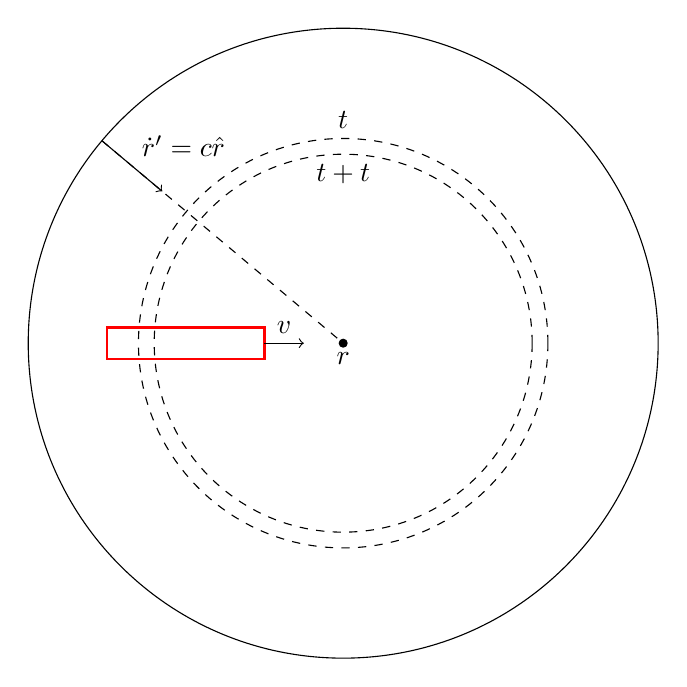
\begin{tikzpicture}
        \pgfmathsetmacro{\boxh}{1.0}
        \pgfmathsetmacro{\boxv}{0.2}
        \pgfmathsetmacro{\R}{4}
        \draw[] (0,0) circle (\R);
        \draw[dashed] (0,0) circle (\R*0.65);
        \draw[dashed] (0,0) circle (\R*0.6);
        \draw[] (0,0+\R*0.65) node[above]{$t$};
        \draw[] (0,0+\R*0.6) node[below]{$t + \dif t$};
        \draw[red, thick] (-2 + \boxh,0 + \boxv) -- (-2 - \boxh,0 + \boxv) -- (-2 - \boxh,0 - \boxv) -- (-2 + \boxh,0 - \boxv) -- cycle;
        \draw[red] (-2, 0) node[]{$\la$};
        \draw[->] (-2 + \boxh, 0) -- node[above]{$\ve v$}(-2 + \boxh + 0.5, 0);
        \draw[fill] (0,0) circle (0.05) node[below]{$\ve r$};
        \draw[dashed] ({-\R*cos(40)}, {\R*sin(40)}) -- (0,0);
        \draw[->] ({-\R*cos(40)}, {\R*sin(40)}) -- node[above right]{$\dot{\ve r}' = c \hat r$} ({-(\R- 1)*cos(40)}, {(\R- 1)*sin(40)});
    \end{tikzpicture}
\end{center}
If the charge is stationary the amount of charge crossed by the ICS in time $\dif t$ would be,
\[ \dif q = \la \dif \rcurs = c \la \dif t \]
But since the charge is moving towards the field point we have instead\footnote{Note that is the sphere were moving inward, the effect would be $1 + v /c$.},
\[ \dif q = \la \br{\dif \rcurs - v \dif t} = \la \br{1 - \f{v}{c}} \dif \rcurs \]
In this case we have,
\[ \f{\la \dif \rcurs}{\rcurs} = \f{\dif q}{\rcurs \br{1 - \f{v}{c}}} \]
Since the potential is due to the charge distribution $\la \br{x', t'}$ we get,
\begin{align*}
    V\br{x,t}
    &= \f{1}{4\pi\ep_0} \int \f{\la \dif \rcurs}{\rcurs} \\
    &= \f{1}{4\pi\ep_0} \int \f{\dif q}{\rcurs \br{1 - \f{v}{c}}} \\
    &= \f{q}{4\pi\ep_0 \rcurs \br{1 - \f{v}{c}}}
\end{align*}
We see that the potential is increased by a factor of $\br{1 - v/c}^{-1}$. This is a \textit{geometric} effect and is independent of the size and/or shape of the charge distribution (despite what this derivation suggests). \\

As the ICS sweeps past the charge it ``sees'' approaching charge for \footnote{See also Feynman's lectures VII, Section 21.5 and Griffiths Section 10.3 p. 451.}. This result can be generalized for a point charge to the \term{Liénard-Wiechert potential},
\[ V\br{\ve r, t} = \f{qc}{4 \pi \ep_0 \ve \rcurs \cdot \br{c \hat \rcurs - \ve v}} \]
and similarly to,
\[ \ve A \br{\ve r, t} = \f{\ve v}{c} V\br{\ve r, t} = \f{\mu_0}{4 \pi}\f{q \ve v}{\ve \rcurs \cdot \br{c \hat \rcurs - \ve v}} \]

\textbf{Griffith Ex. 10.3:} Find the potential of a point charge moving with a constant velocity. Let the course position be,
\[ \ve r' \br{t'} = \ve v t' \]
so that it is at the origin at $t = 0$. The retarded time is (recall $t = t' - \rcurs / c$),
\[ t' = t + \f{\rcurs}{c} \]
Which gives,
\[ \rcurs =c\br{t' - t} = \abs{\ve r - \ve r'} \]
so that we have,
\begin{align*}
c^2 \br{t^2 - 2tt' + t'^2}
&= r^2 +r'^2 - 2 \ve r\cdot \ve r' \\
&= r^2 + v^2 t'^2- 2 t' \ve r \cdot \ve v \\
0 &= \br{v^2 - c^2} t'^2 + \br{2 c^2 t - 2 \ve r \cdot \ve v} t' + \br{r^2 - c^2 t^2}
\end{align*}
Solving the quadratic for $t'$,
\[ t' = \f{\br{c^2 t - \ve r \cdot \ve v} \pm \sqrt{\br{c^2 t - \ve r \cdot \ve v}^2 - \br{v^2 - c^2}\br{r^2 - c^2 t^2}}}{-v^2 + c^2}\]
What sign is physically appropriate? If we have $v = 0$,
\[ t' = \f{\br{c^2 t} \pm \sqrt{\br{c^2 t}^2 - \br{c^2}\br{r^2 - c^2 t^2}}}{c^2} = t\pm \f{r}{c}\]
Physically, the upper ($+$) solution corresponds to an incorrect expression for the retarded time, namely $t' = t + \rcurs / c$. This corresponds to retrocausation and thus should be discarded on the basis of causality. We take the lower sign solution ($-$). We can write the discriminant,
\[ \sqrt{\br{c^2 t - \ve r \cdot \ve v}^2 - \br{v^2 - c^2}\br{r^2 - c^2 t^2}} = \br{c^2 t - \ve r \cdot \ve v} - \br{c^2 - v^2} t' \]
From,
\[ \hat \rcurs = \f{\ve r - \ve r'}{\abs{\ve r' - \ve r'}}= \f{\ve r - \ve v t}{c\br{t - t'}} \]
And consider,
\begin{align*}
c\rcurs \br{1 - \hat \rcurs \cdot \f{\ve v}{c}}
&= c^2 \br{t - t'} \br{1 - \f{\ve v}{c} \cdot \f{\br{\ve r - \ve v t}}{c \br{t - t'}}} \\
&= c^2 \br{t - t'} -  \ve v \cdot \ve r - v^2 t' \\
&= \br{c^2 t - \ve r \cdot \ve v} - \br{c^2 - v^2 }t'
\end{align*}
And finally,
\[ V\br{\ve r, t}= \f{c}{4 \pi \ep_0} \f{q}{\sqrt{\br{c^2 t - \ve r \cdot \ve v}^2 + \br{c^2 - v^2}\br{r^2 - c^2 t^2}}} \]
And the vector potential is simply,
\[ \ve A \br{\ve r, t} = \f{\ve v V}{c} \]
\textbf{Griffith Ex. 10.3:} The fields of a moving point charge are,
\[ \ve E \br{\ve r, t} = \f{q}{4 \pi \ep_0} \f{\rcurs}{\br{\ve \rcurs \cdot \ve u}^3} \bc{\br{c^2 - v^2} \ve u + \ve \rcurs \times \br{\ve u \times \ve a}} \]
Where $\ve u$ is shorthand,
\[ \ve u = c \hat \rcurs - \ve v \]
And $\ve a$ is the acceleration,
\[ \ve a = \dot{\ve v} \]
The magnetic field can be obtained via,
\[ \ve B\br{\ve r, t} = \f{\hat \rcurs}{c} \times \ve E \]

\section{Radiation}

We have the the \term{Jefimenko} equations,
\[ \ve E \br{\ve r, t} = \f{1}{4 \pi\ep_0} \int \dif \tau' \br{\f{\rho \hat \rcurs}{\rcurs^2} + \f{\dot \rho \hat \rcurs}{c \rcurs}- \f{\ve J}{c^2 \rcurs}}  \]
\[ \ve B \br{\ve r, t} = \f{\mu_0}{4 \pi} \int \dif \tau' \br{\f{\ve J}{\rcurs^2} + \f{\dot {\ve J}}{c \rcurs}}\times \hat \rcurs \]
So the Poynting vector is $\ve S = \f{1}{\mu_0} \ve E \times \ve B$ and the power is,
\[ P\br{\ve r, t} = \oint \dif \ve a \cdot \ve S = \f{1}{\mu_0} \int \dif \ve a \cdot \ve E\times \ve B \]
When considering radiation, we are only concerned with the far-field affects ($\rcurs \to \inf$) so that only the terms $\sim \f{1}{\rcurs}$ remain (because the areas increases as $\rcurs^2$). This chapter is concerned largely with this \textit{far field limit}. In the limit, energy leaves the sources and does \textit{not} return. \\

\subsection{Electric Dipole}
First, consider the problem of an electric dipole connected by a wire of length $d$.

\begin{center}
    \begin{tikzpicture}
        \coordinate (qp) at (0, 2);
        \coordinate (qm) at (0, -2);
        \coordinate (f) at (4, 2.5);
        \draw[->] (0, 0) -- (5, 0) node[right]{$y$};
        \draw[->] (0, -3) -- (0, 3) node[above]{$z$};
        \draw[|<->|] ([xshift=-1em]qm) -- node[left]{$d$} ([xshift=-1em]qp);
        \draw[fill] (qp) circle (0.05) node[above right]{$q_+$};
        \draw[fill] (qm) circle (0.05) node[below right]{$q_-$};
        \draw[->] (qp) -- node[above]{$\brcurs_+$} (f);
        \draw[->] (qm) -- node[right]{$\brcurs_-$} (f);
        \draw[->] (0,0) -- node[above]{$\ve r$} (f);
        \draw (0,0.75) node[below right]{$\te$} arc (90:32:0.75);
    \end{tikzpicture}
\end{center}

Where the charge is anti-symmetrically distributed and oscillating with frequency $\w$.
\[ q_{\pm}\br{t} = \pm q_0 \cos \br{\w, t} \]
As a result, the electric potential generated by each charge at position $\ve r$ and time $t$ is retarded by the speed of light.
\[ V\br{\ve r, t} = V_+\br{\ve r, t} + V_-\br{\ve r, t} = \f{q_0}{4\pi\ep_0} \bc{\f{\cos\bs{\w\br{t- \rcurs_+/c}}}{\rcurs_+} - \f{\cos\bs{\w\br{t- \rcurs_-/c}}}{\rcurs_-}} \eq \label{eq:potential}\]
Since we are only interested in the contributions to the field at very large distances $r \gg d$, we can approximate the distance between the field and source,
\[ \rcurs_{\pm} = \sqrt{r^2 \mp rd\cos\te + \br{d/2}^2} \simeq r\br{1\mp \f{d}{2r}\cos \te} \qquad \br{d \ll r}\]
Similarly we have,
\[ \f{1}{\rcurs_{\pm}} = \simeq \f{1}{r}\br{1\pm \f{d}{2r}\cos \te} \qquad \br{d \ll r} \eq \label{eq:approx_1}\]
Therefore we have that,
\begin{align*}
\cos\bs{\w\br{t - \rcurs_{\pm}/c}}
&\simeq \cos\bs{\w\br{t - \f{r}{c}\br{1\mp \f{d}{2r}\cos \te}}} \qquad {\text{Substitution}}\\
&= \cos\bs{\w\br{t - \f{r}{c} \pm \f{d}{2c}\cos \te}} \qquad {\text{Rearrangement}}\\
&= \cos\bs{\w\br{t - \f{r}{c}}}\cos\bs{\f{\w d}{2c}\cos \te} \mp \sin\bs{\w\br{t - \f{r}{c}}}\sin\bs{\f{\w d}{2c}\cos \te} \qquad {\text{Trig Identity}}
\end{align*}
For a perfect dipole, we not only have $d \ll r$ but that $d \ll \la = 2 \pi c / \w$. Therefore we can perform small angle approximations for $\f{\w d}{2c}$ terms,
\[ \cos\bs{\w\br{t - \rcurs_{\pm}/c}} \simeq \cos\bs{\w\br{t - \f{r}{c}}} \mp \sin\bs{\w\br{t - \f{r}{c}}}\f{\w d}{2c}\cos \te \eq \label{eq:cos_approx}\]
Combining \cref{eq:approx_1,eq:cos_approx} into \cref{eq:potential} gives,
\[ V\br{r, \te, t} = \f{q_0 d \cos \te}{4\pi \ep_0 r} \bc{- \f{\w}{c} \sin\bs{\w\br{t - r/c}} + \f{1}{r}\cos\bs{\w\br{t - r/c}}} \]
Finally, we may approximate the large distance to wavelength approximation $r \gg \la$ which means that $\f{1}{r} \ll \f{\w}{c}$. Therefore we may neglect the cosine contribution and arrive at,
\[ V\br{r, \te, t} = -\f{q_0 d \cos \te}{4\pi \ep_0 r}\f{\w}{c} \sin\bs{\w\br{t - r/c}} \eq \label{eq:V}\]

Similarly we can calculate the current flowing through the wire of length $d$. The current must accommodate the charge,
\[ \ve I \br{t} = \der{q}{t}\hat z = - q_0 \w \sin \br{\w t} \hat z \eq \label{eq:current} \]
Therefore the vector potential is the integral over the retarded current contributions.
\[ \ve A \br{\ve r, t} = \f{\mu_0}{4 \pi} \int_{-d/2}^{d/2} \f{- q_0 \w \sin\bs{\w\br{t - \rcurs / c}} \hat z}{\rcurs} \dif z \]
Since $d \ll r$, the difference $(+ d/2 \hat z) - (- d/2 \hat z)$ is nearly $\dif z \hat z$. Therefore $\rcurs \simeq r$,
\[ \ve A \br{r, \te, t} \simeq \f{\mu_0}{4 \pi} \f{- q_0 \w \sin\bs{\w\br{t - r / c}} \hat z}{r} \eq\label{eq:A}\]
Simple algebra can be performed to calculate $\ve E, \ve B$ from $V, \ve A$.
\begin{align*}
\vdel V
&= \pder{V}{r} \hat r + \f{1}{r} \pder{V}{\te} \hat \te \\
&= -\f{q_0 d \w}{4 \pi \ep_0 c} \bc{\cos \te \br{- \f{1}{r^2} \sin \w t' - \f{\w}{rc} \cos \w t'} \hat r - \f{\sin \te}{r^2}\sin\w t' \hat \te }\\
&\simeq \f{q_0 d \w^2}{4 \pi \ep_0 c^2} \br{\f{\cos \te}{r}} \cos \w t' \hat r \qquad \la \ll r \eq \label{eq:gradV}
\end{align*}
The time dependence on $\ve A$ is,
\[ \pder{\ve A}{t} = - \f{\mu_0 q_0 d \w^2}{4 \pi r} \cos \w t' \br{\cos \te \hat r - \sin \te \hat \te} \eq\label{eq:tA}\]
\Cref{eq:gradV,eq:tA} fix the electric field,
\[ \ve E = - \vdel V - \pder{\ve A}{t} \simeq \f{\mu_0 q_0 d \w^2}{4 \pi} \br{\f{\sin \te}{r}}\cos \w t'\hat \te \eq \label{eq:E}\]
While $\vdel \times \ve A$ fixes $\ve B$,
\begin{align*}
\vdel \times \ve A
&= \f{1}{r} \bs{\pder{}{r} \br{r A_\te} - \pder{A_r}{\te}}\hat\phi \\
&= \f{1}{r} \pder{}{r} \br{r A \sin \te}\hat\phi \\
&= \f{\mu_0 q_0 d \w}{4 \pi r} \bc{\f{\w}{c} \sin \te \cos \w t' + \f{\sin \te}{r} \sin \w t'}\hat \phi \\
&= \f{\mu_0 q_0 d \w^2}{4 \pi c} \br{\f{\sin \te}{r}} \cos \w t'\hat \phi \qquad \la \ll r
\end{align*}
Therefore,
\[ \ve B = \vdel \times \ve A = \f{\mu_0 q_0 d \w^2}{4 \pi c} \br{\f{\sin \te}{r}} \cos \w t'\hat \phi \eq \label{eq:B} \]
Combining \cref{eq:E} and \cref{eq:B} one can calculate the Poynting vector,
\[ \ve S \br{\ve r, t} = \f{1}{\mu_0} \br{\ve E \times \ve B} = \f{\mu_0}{c} \bc{\f{q_0 d \w^2}{4 \pi}\br{\f{\sin \te}{r}} \cos \w t'}^2 \hat r \]
Therefore the time averaged Poynting vector yields the intensity,
\[ \ba{\ve S} = \br{\f{\mu_0 q_0^2 d^2 \w^4}{32 \pi^2 c}}\f{\sin^2 \te}{r^2} \hat r \eq \label{eq:as_before}\]
Therefore the total power radiating at $r \gg d$ over all directions,
\[ \ba{P} = \intl_{0}^{\pi} \dif \te \intl_{0}^{2 \pi} \dif \phi \ba{\ve S} \cdot \hat r r^2 \sin \te = \f{\mu_0 q_0^2 d^2 \w^4}{12 \pi c} \eq \label{eq:dipole_radiation_power}\]

In summary, we have for electric dipole radiation $p_0 = q_0 d$:
\[ \ve E\br{\ve r, t} =  \f{\mu_0 p_0 \w^2}{4 \pi} \br{\f{\sin \te}{r}}\cos \bc{\w \br{t - r/ c}}\hat \te\]
\[ \ve B\br{\ve r, t} =  \f{\mu_0 p_0 \w^2}{4 \pi c} \br{\f{\sin \te}{r}} \cos \bc{\w \br{t - r/ c}}\hat \phi \]
Using \textbf{three} assumptions:
\[ d \ll \rcurs \qquad d \ll \f{\la}{2\pi} \qquad \rcurs \gg \f{\la}{2 \pi} \]

\subsection{Magnetic Dipole}
The magnetic dipole consists of an loop of radius $b$ carrying current,
\[ I\br{t} = I_0 \cos \br{\w t} \]
The magnetic dipole problem is remarkably very similar to the electric dipole problem. Most of the equations and approximations hold under the following mapping,
\[ d \approx b \qquad I_0 \times \f{2 \pi b}{c} \approx q_0 \]
Which together amount to,
\begin{align*}
    q_0 d c \propto \pi b^2 I_0
\end{align*}
Which relates length and time scales together. The key difference being that the potential is zero because the charge density is constant.
The vector potential is the integral over the retarded current contributions.
\[ \ve A \br{\ve r, t} = \f{\mu_0}{4 \pi} \int \f{I_0 \cos\bs{\w\br{t - \rcurs / c}}}{\rcurs} \dif \ve \ell' \]
Where $\dif \ve \ell' = b \dif \phi' \hat \phi = b \cos \phi' \dif \phi'\hat y - b \sin \phi'\dif \phi' \hat x$. Hence,
\[ \ve A \br{\ve r, t} = \f{b\mu_0}{4 \pi} \int_{0}^{2\pi} \f{I_0 \cos\bs{\w\br{t - \rcurs / c}}}{\rcurs} \bc{\cos \phi'\hat y - \sin \phi' \hat x} \dif \phi' \eq \label{eq:A_magnetic_dipole}\]
Without loss of generality we can place the field point above the $x$-axis such that the field point and loop points be respectively,
\[ \ve r = r \sin \te \hat x + r \cos \te \hat z \qquad \ve b = b \cos \phi' \hat x + b \sin \phi' \hat y \]
Again by cosine law,
\[ \rcurs = \sqrt{r^2 + b^2 - 2 r b \cos \psi_{r,b}} \]
Where $\psi_{r,b}$ is the oblique angle between $\ve b$ and $\ve r$. Hence know that $r b \cos \psi_{r, b} = \ve r \cdot \ve b = rb \sin \te \cos \phi'$. Therefore,
\[ \rcurs = \sqrt{r^2 + b^2 - 2 r b \sin \te \cos \phi'} \]
Analogous to the electric dipole case we make the far field approximation,
\[ b \ll r \]
Therefore,
\[ \rcurs \simeq r\br{1 - \f{b}{r}\sin \te \cos \phi'} \]
And,
\[ \f{1}{\rcurs} \simeq \f{1}{r}\br{1 + \f{b}{r}\sin \te \cos \phi'} \]
Therefore if we make the frequency approximation $b \ll \la \propto \f{c}{\w}$,
\begin{align*}
    \cos \bs{\w\br{t - \rcurs/ c}}
    &\simeq \cos\bs{\w \br{t - \rcurs /c} + \f{wb}{c} \sin \te \cos \phi'} \\
    &= \cos\bs{\w \br{t - \rcurs /c}}\cos\bs{\f{wb}{c} \sin \te \cos \phi'} - \sin\bs{\w \br{t - \rcurs /c}}\sin\bs{\f{wb}{c} \sin \te \cos \phi'} \\
    &\simeq \cos\bs{\w \br{t - \rcurs /c}} - \f{wb}{c}\sin\bs{\w \br{t - \rcurs /c}} \sin \te \cos \phi' \qquad b \ll \f{c}{\w}
\end{align*}
We can now approximately perform the integral of \cref{eq:A_magnetic_dipole},
\[ \ve A\br{\ve r, t} \simeq \f{\mu_0 I_0 b}{4 \pi r} \intl_{0}^{2\pi} \bc{\br{1 + \f{b}{r}\sin \te \cos \phi'} \times \br{\cos \w t' - \f{\w b}{c} \sin \w t' \sin \te \cos \phi'}} \bc{\cos \phi'\hat y - \sin \phi' \hat x} \dif \phi' \]
Only a few terms have non-zero contribution under an integral over $\phi' \in \bs{0, 2\pi}$. Namely those quadratic in $\cos \phi'$. Therefore the $\hat x$ terms do not contribute and $\ve A$ points in the $\hat y$ direction (however this was under the assumption that the field point is above the $x$-axis; in general the $\ve A$ potential would point in the $\hat phi$ direction),
\[ \ve A\br{r, \te, t} \simeq \f{\mu_0 I_0 \pi b^2}{4 \pi}\br{\f{\sin \te}{r}} \bc{\f{1}{r} \cos \w t' - \f{\w}{c} \sin \w t'}\hat\phi \eq \label{eq:A_mag_no_approx}\]
We may again use the third and final approximation that $r \gg \la \propto \f{c}{\w}$ to obtain,
\[ \ve A\br{r, \te, t} \simeq -\f{\mu_0 I_0 \pi b^2 \w}{4 \pi c}\br{\f{\sin \te}{r}} \sin \bc{\w \br{t - r/c}} \hat\phi \eq \label{eq:A_mag}\]
Therefore the electric and magnetic fields can be calculated directly,
\begin{align*}
    \ve E &= - \pder{\ve A}{t} \simeq \f{\mu_0 I_0 \pi b^2 \w^2}{4 \pi c} \br{\f{\sin \te}{r}} \cos \bc{\w \br{t - r/c}}\hat \phi \\
    \ve B &= \vdel \times \ve A \simeq \f{\mu_0 I_0 \pi b^2 \w^2}{4 \pi c^2} \br{\f{\sin \te}{r}} \cos \bc{\w \br{t - r/c}}\hat \te
\end{align*}
Note that $m_0 = \pi I_0 b^2$ is often written instead. From the fields, calculate the Poynting vector,
\[ \ve S \br{\ve r, t} = \f{1}{\mu_0} \br{\ve E \times \ve B} = \f{\mu_0}{c} \bc{\f{I_0 \pi b^2 \w^2}{4 \pi c}\br{\f{\sin \te}{r}} \cos \w t'}^2 \hat r \]
Therefore the time averaged Poynting vector yields the intensity,
\[ \ba{\ve S} = \br{\f{\mu_0 I_0^2 \pi^2 b^4 \w^4}{32 \pi^2 c^3}}\f{\sin^2 \te}{r^2} \hat r \]
Therefore the total power radiating at $r \gg d$ over all directions,
\[ \ba{P} = \intl_{0}^{\pi} \dif \te \intl_{0}^{2 \pi} \dif \phi \ba{\ve S} \cdot \hat r r^2 \sin \te = \f{\mu_0 I_0^2 b^4 \w^4}{12 \pi c^3} \eq \label{eq:mag_dipole_radiation_power}\]

Comparing the power radiated from the electric dipole with the magnetic dipole,
\[ \f{\ba{P}_{m}}{\ba{P}_{e}} = \br{\f{m_0}{p_0c}}^2 \]

\subsection{Radiation from an Arbitrary Source}

Considering the case of a generic, localized blob of charge $\rho\br{\ve r, t}$ we have,
\[ V\br{\ve r, t} = \f{1}{4 \pi \ep_0} \int \dif \tau' \f{\rho\br{\ve r', t'}}{\rcurs} \]
Where $t' = t - \rcurs / c$. Here we make the far-field approximation of $r' \ll r$ and $r' \ll \la / 2 \pi$. It can be shown that under these two approximations,
\[ V\br{\ve r, t} = \f{1}{4 \pi \ep_0} \br{\f{Q}{r} + \f{\hat r \cdot \ve p \br{t'}}{r^2} + \f{\hat r \cdot \dot {\ve p}\br{t'}}{cr}} \Bigg|_{t' = t - \rcurs / c} \]
And similarly,
\[ \ve A\br{\ve r, t} = \f{\mu_0}{4 \pi} \dot {\ve p}\br{t - \rcurs / c}  \]
The electric field is,
\[ \ve E\br{\ve r, t} = \f{\mu_0}{4 \pi r} \bc{\br{\hat r \cdot \ddot{\ve p}}\hat r - \ddot{\ve p}} = - \f{\mu_0}{4 \pi r} \ddot{\ve p}_{\perp}\br{t'} \]
Where $\ddot{\ve p}_{\perp} = \hat r \times \br{\ddot{\ve p} \times \hat r}$ is the component of $\ddot{\ve p}$ perpendicular to $\hat r$.
\[ \ve B\br{\ve r, t} = - \f{\mu_0}{4 \pi r c} \hat r \times \ddot{\ve p} \br{t'}  \]
Notice that $\ve E = - c \hat r \times \ve B$. The Poynting vector is,
\[ \ve S \br{\ve r, t} = \f{\mu_0}{16 \pi^2 c} \br{\f{\ddot p \br{t'} \sin \te }{r}}^2 \hat r\]
Where $\ddot{\ve p} = \ddot p \hat z$. The power radiated out to infinity is,
\[ \ba{P} = \oint \ve S \cdot \dif \ve a = \f{\mu_0}{6 \pi c} \ddot p^2 \br{t'} \]
For $\ddot p = q a$ (where $a$ is the acceleration of a charge $q$),
\[ \ba{P} = \f{\mu_0 q^2 a^2}{6 \pi c} \]
Which is the famous \term{Larmor formula}.

\section{Special Relativity}

\subsection{The Origins of SR}

In 1864, we had Maxwell's equations which when rearranged gave wave equations such as,
\[ \del^2 \ve E = - \mu_0 \ep_0 \pdder{\ve E}{t} \]
With wavespeed $c = 1 / \sqrt{\mu_0 \ep_0}$. However, Maxwell's equations do not obey Galilean relativity; a uniformly moving reference frame traveling at $\ve v$ gives the wavespeed $\ve c + \ve v$. At this time, it was believed that a wave required a mediator for propagation to occur and so the ``ether'' was hypothesized. One would imagine measuring the ether by using earth's motion. Earth's velocity through the ether is,
\[ \f{2 \pi \br{\SI{1}{\AU}}}{\SI{1}{\yr}} \simeq \SI{30}{\kilo\m\per\s} \simeq \SI{e-4}{}\text{c} \]
Michaelson \& Morley set out to measure this and had a null result. There were several pre-special relativity attempts to explain this null result, the most famous by George Fitzgerald and Lorentz who obtained the mathematical form of how Maxwell's equations in different inertial reference frames must transform, but were unable to come up with a physical model.\\

In 1889, Fitzgerald proposed a length contraction to account for this,
\[ \ga = \f{1}{\sqrt{1 - \br{\f{v}{c}}^2}} \]

Shortly after, Einstein came up with SR.\\

\textbf{Postulates:}
\begin{enumerate}
    \item The laws of physics are the same in all inertial reference frames
    \item The speed of light is the same in all inertial reference frames
\end{enumerate}

With these postulates he replaced Galilean transformations with Lorentz transformations.

\newcommand{\sqm}[1]{\begin{bmatrix}#1\end{bmatrix}}
\newcommand{\p}[1]{\texttt{#1}}
\definecolor{lightcolor}{HTML}{CCCC00}
\newcommand{\arcd}[4]{% height, angle1, angle2, label
\draw[<->] (90-#2:#1)
    arc[radius=#1, start angle=90-#2, end angle=90-(#3 + #2)/2]
    node[above] {#4}
    arc[radius=#1, start angle=90-(#3 + #2)/2, end angle=90-#3]
}
\newcommand{\spacetime}[5]{ % maxx maxy ar br
    \begin{center}
    \begin{tikzpicture}[every path/.style={thick}]
        \pgfmathsetmacro{\maxx}{#1};
        \pgfmathsetmacro{\maxt}{#2};
        \pgfmathsetmacro{\ar}{#3};
        \pgfmathsetmacro{\br}{#4};
        \coordinate (x) at (\maxx, 0);
        \coordinate (t) at (0, \maxt);
        \coordinate (o) at (0, 0);
        \draw[gray, dashed] (o) -- ($(x)+(t)$) coordinate (u_r);
        \draw[blue, ->] (o) -- ([rotate=-\br]t) coordinate (t_p) node[above]{$t'$};
        \draw[blue, ->] (o) -- ([rotate=+\br]x) coordinate (x_p) node[right]{$x'$, \p{B}};
        \draw[red, ->]  (o) -- ([rotate=-\ar]t) coordinate (t)   node[above]{$t$};
        \draw[red, ->]  (o) -- ([rotate=+\ar]x) coordinate (x)   node[right]{$x$, \p{A}};
        #5
    \end{tikzpicture}
    \end{center}
}
\newcommand{\spacetimeneg}[5]{ % maxx maxy ar br
    \begin{center}
    \begin{tikzpicture}[every path/.style={thick}]
        \pgfmathsetmacro{\maxx}{#1};
        \pgfmathsetmacro{\maxt}{#2};
        \pgfmathsetmacro{\ar}{#3};
        \pgfmathsetmacro{\br}{#4};
        \coordinate (x) at (\maxx, 0);
        \coordinate (t) at (0, \maxt);
        \coordinate (o) at (0, 0);
        \draw[gray, dashed] ($-1*(x)-1*(t)$) -- ($(x)+(t)$) coordinate (u_r);
        \draw[blue, ->] ([rotate=180-\br]t) coordinate (n_t_p) -- ([rotate=-\br]t) coordinate (t_p) node[above]{$t'$};
        \draw[blue, ->] ([rotate=180+\br]x) coordinate (n_x_p) -- ([rotate=+\br]x) coordinate (x_p) node[right]{$x'$, \p{B}};
        \draw[red, ->]  ([rotate=180-\ar]t) coordinate (n_t)   -- ([rotate=-\ar]t) coordinate (t)   node[above]{$t$};
        \draw[red, ->]  ([rotate=180+\ar]x) coordinate (n_x)   -- ([rotate=+\ar]x) coordinate (x)   node[right]{$x$, \p{A}};
        #5
    \end{tikzpicture}
    \end{center}
}
\subsection{Galileo Diagrams}

Consider next a \term{Galileo diagram} where with two observers $\p A$ and $\p B$ with relative speed $v$ such that $\tan \phi = v/c$ and the event $E$,

\begin{center}
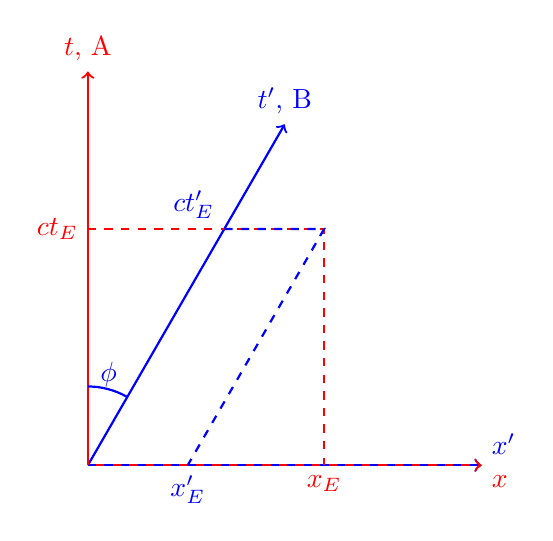
\begin{tikzpicture}[every path/.style={thick}]
    \pgfmathsetmacro{\maxx}{5};
    \pgfmathsetmacro{\maxt}{5};
    \pgfmathsetmacro{\ar}{0};
    \pgfmathsetmacro{\br}{30};
    \pgfmathsetmacro{\Ax}{3};
    \pgfmathsetmacro{\Ay}{3};
    \coordinate (x) at (\maxx, 0);
    \coordinate (t) at (0, \maxt);
    \coordinate (o) at (0, 0);
    \draw[blue, ->] (o) -- ([rotate=-\br]t) node[above]{$t'$, \p{B}};
    \draw[blue, ->, dashed, dash phase=0pt] (o) -- ([rotate=0]x) node[above right]{$x'$};
    \draw[red, ->] (o) -- ([rotate=-\ar]t) node[above]{$t$, \p{A}};
    \draw[red, ->, dashed, dash phase=3pt] (o) -- ([rotate=0]x) node[below right]{$x$};
    \draw[dashed, red] (0, \Ay) node[left]{$ct_{E}$} -- (\Ax, \Ay) -- (\Ax, 0) node[below]{$x_{E}$};
    \draw[dashed, blue] (\Ay*tan{\br}, \Ay) node[above left]{$ct_{E}'$} -- (\Ax, \Ay) -- (\Ax - \Ay*tan{\br}, 0) node[below]{$x_{E}'$};
    \draw[blue] (0, 1) arc (90:90-\br:1) node[above left]{$\phi$};
\end{tikzpicture}
\end{center}

Setting $c = 1$, the coordinates of \p{B} with respect to \p{A} when using a Galilean transformation are,
\[ \sqm{x' \\ t'} = \sqm{1 & - v \\ 0 & 1} \sqm{x \\ t} = \sqm{x - v t \\ t} \]
For the event $E$ in the Galileo diagram, we have the following transformations,
\[ x_E' = x_E - v t_E \qquad t_E = t_E' \]
Notice how the time coordinates of each observer are the same.

However, under a Lorentz transformation, we have a different perspective.

\begin{center}
  \begin{minipage}[b]{0.45\textwidth}
    \spacetime{5}{5}{0}{30}{
        \pgfmathsetmacro{\arch}{2};
        \arcd{1*\arch}{\br}{\ar}{$\al$};
    }
    \begin{center}
    $\p A$'s reference frame.
    \end{center}
  \end{minipage}
  \begin{minipage}[b]{0.45\textwidth}
    \spacetime{5}{5}{-30}{0}{
        \pgfmathsetmacro{\arch}{2};
        \arcd{1*\arch}{\br}{\ar}{$\al$};
    }
    \begin{center}
    $\p B$'s reference frame.
    \end{center}
  \end{minipage}
\end{center}

In Minkowski space, light travels at speed $c$ in all inertial references frames. The light cone doesn't change between reference frames.

\subsection{Simultaneity}

Under Lorentz transformations, simultaneity becomes dependent on the reference frame. Consider two events $1$, $2$ that are synchronized in $\p A$'s frame. In $\p B$'s frame however, these events occur at two different times $t_1' \neq t_2'$. \\

Since \p{B} is moving at speed $v$ to the right relative to \p{A}, the Lorentz transformation is,
\[ \sqm{x' \\ ct'} = \ga\sqm{1 & -v / c \\ -v /c & 1} \sqm{x \\ ct} = \ga \sqm{x - v t \\ -v /c x + c t} \]
Suppose \p{A} measures the ends of the clock simultaneously at $t = 0$. Therefore,
\[ \sqm{x' \\ ct'} = \ga \sqm{x \\- v /c x}  \]
Explicitly,
\begin{align*}
x'_1 &= \ga x_1 \\
x'_2 &= \ga x_2 \\
t'_1 &= -\ga \f{v}{c^2} x_1 \\
t'_2 &= -\ga \f{v}{c^2} x_2
\end{align*}
Which implies the following,
\begin{align*}
\De x_{\p{B}} = \De x' &= \ga \De x = \ga \De x_{\p{A}} \\
\De t_{\p{B}} = \De t' &= -\ga \f{v}{c^2} \De x = -\ga \f{v}{c^2} \De x_{\p{A}}
\end{align*}
Therefore we have discovered \term{length contraction}. In the reference frame of \p{A},
\[ \De x_{\p{B}} = \f{1}{\sqrt{1 - v^2 /c^2}} \De x_{\p{A}} \geq \De x_{\p{A}}\]

\newcommand{\qqx}[2]{
\spacetimeneg{5}{5}{#1}{#2}{
    \draw[dashed, gray] (-\maxx, \maxt) -- (\maxx, - \maxt);

    \pgfmathsetmacro{\dtx}{1/5};
    \pgfmathsetmacro{\ray}{5};

    \coordinate (E) at ($\dtx*(x)$);
    \coordinate (E2) at ($2*\dtx*(x)$);
    \coordinate (Eray) at ($(E) + (\ray, \ray)$);
    \coordinate (Eray2) at ($(E2) + (\ray, \ray)$);
    \coordinate (EonB) at (intersection of n_x_p--x_p and E--Eray);
    \coordinate (EonB2) at (intersection of n_x_p--x_p and E2--Eray2);
    \draw[red, |-|] (E) node[below]{$x_1$} --  (E2) node[below]{$x_2$};

    \draw[lightcolor, ->] (E) -- (EonB);
    \draw[lightcolor, ->] (E2) -- (EonB2);

    \coordinate (EponBx) at ($(E) - (t_p)$);
    \coordinate (EonBx) at (intersection of n_x_p--x_p and E--EponBx);
    \draw[dashed, thin, blue] (E) -- (EonBx) ;
    \coordinate (EponBx2) at ($(E2) - (t_p)$);
    \coordinate (EonBx2) at (intersection of n_x_p--x_p and E2--EponBx2);
    \draw[dashed, thin, blue] (E2) -- (EonBx2) ;
    \draw[blue, |-|] (EonBx) node[above]{$x'_1$} -- (EonBx2) node[above]{$x'_2$};

    \coordinate (EponBt) at ($(E) + (x_p)$);
    \coordinate (EonBt) at (intersection of n_t_p--t_p and E--EponBt);
    \draw[dashed, thin, blue] (E) -- (EonBt) ;
    \coordinate (EponBt2) at ($(E2) + (x_p)$);
    \coordinate (EonBt2) at (intersection of n_t_p--t_p and E2--EponBt2);
    \draw[dashed, thin, blue] (E2) -- (EonBt2) ;
    \draw[blue, |-|] (EonBt) node[left]{$t'_1$} -- (EonBt2) node[left]{$t'_2$};

    \draw[fill] (E) circle[radius=0.05];
    \draw[fill] (E2) circle[radius=0.05];
}
}

\qqx{0}{28}
\begin{center}
$\p A$'s reference frame.
\end{center}
\qqx{-28}{0}
\begin{center}
$\p B$'s reference frame.
\end{center}
\qqx{-14}{14}
\begin{center}
Between $\p A$'s and $\p B$'s reference frame.
\end{center}

\subsection{Proper Time}

Under Lorentz transformations, locality becomes dependent on the reference frame. Consider two events $1$, $2$ that occur at the same place in $\p A$'s frame. In $\p B$'s frame however, these events occur at two different places $x_1' \neq x_2'$. \\

Since \p{B} is moving at speed $v$ to the right relative to \p{A}, the Lorentz transformation is,
\[ \sqm{x' \\ ct'} = \ga\sqm{1 & -v / c \\ -v /c & 1} \sqm{x \\ ct} = \ga \sqm{x - v t \\ - v /c x + c t} \]
The first and second ticks occur on \p{A}'s clock at $x = 0$. Therefore,
\[ \sqm{x' \\ ct'} = \ga \sqm{- v t \\ c t} \]
Explicitly,
\begin{align*}
x'_1 &= -\ga v t_1 \\
x'_2 &= -\ga v t_2 \\
t'_1 &= \ga t_1 \\
t'_2 &= \ga t_2
\end{align*}
Which implies the following,
\begin{align*}
\De x_{\p{B}} = \De x' &= -\ga v \De t = -\ga v \De t_{\p{A}} \\
\De t_{\p{B}} = \De t' &= \ga \De t = \ga \De t_{\p{A}}
\end{align*}
Therefore we have discovered \term{time dilation}. In the reference frame of \p{A},
\[ \De t_{\p{B}} = \f{1}{\sqrt{1 - v^2 /c^2}} \De t_{\p{A}} \geq \De t_{\p{A}}\]
\p{B} could instead measure $\De \tau_{\p{B}}$ where,
\begin{align*}
c^2\De \tau_\p{B}^2
&= c^2 \De t_\p{B}^2 - \De x_\p{B}^2 \\
&= c^2 \br{\ga \De t_{\p{A}}}^2 - \br{-\ga v \De t_{\p{A}}}^2 \\
&= \ga^2 \br{c^2 - v^2}\De t_{\p{A}}^2 \\
&= c^2 \De t_{\p{A}}^2 \\
&= c^2 \De \tau_{\p{A}}^2
\end{align*}
Therefore \term{proper time} is invariant,
\[ \De \tau_{\p{A}} = \De \tau_{\p{B}} \]
\newcommand{\qqt}[2]{
\spacetimeneg{5}{5}{#1}{#2}{
    \draw[dashed, gray] (-\maxx, \maxt) -- (\maxx, - \maxt);
    \pgfmathsetmacro{\dta}{1/5};
    \pgfmathsetmacro{\ray}{5};

    \coordinate (E) at ($\dta*(t)$);
    \coordinate (E2) at ($2*\dta*(t)$);
    \coordinate (Eray) at ($(E) + (\ray, \ray)$);
    \coordinate (Eray2) at ($(E2) + (\ray, \ray)$);
    \coordinate (EonB) at (intersection of n_t_p--t_p and E--Eray);
    \coordinate (EonB2) at (intersection of n_t_p--t_p and E2--Eray2);
    \draw[red, |-|] (E) node[left]{$t_1$} --  (E2) node[left]{$t_2$};

    \draw[lightcolor, ->] (E) -- (EonB);
    \draw[lightcolor, ->] (E2) -- (EonB2);

    \coordinate (EponBx) at ($(E) - (t_p)$);
    \coordinate (EonBx) at (intersection of n_x_p--x_p and E--EponBx);
    \draw[dashed, thin, blue] (E) -- (EonBx) ;
    \coordinate (EponBx2) at ($(E2) - (t_p)$);
    \coordinate (EonBx2) at (intersection of n_x_p--x_p and E2--EponBx2);
    \draw[dashed, thin, blue] (E2) -- (EonBx2) ;
    \draw[blue, |-|] (EonBx) node[below]{$x'_1$} -- (EonBx2) node[above left]{$x'_2$};

    \coordinate (EponBt) at ($(E) + (x_p)$);
    \coordinate (EonBt) at (intersection of n_t_p--t_p and E--EponBt);
    \draw[dashed, thin, blue] (E) -- (EonBt) ;
    \coordinate (EponBt2) at ($(E2) + (x_p)$);
    \coordinate (EonBt2) at (intersection of n_t_p--t_p and E2--EponBt2);
    \draw[dashed, thin, blue] (E2) -- (EonBt2) ;
    \draw[blue, |-|] (EonBt) node[right]{$t'_1$} -- (EonBt2) node[right]{$t'_2$};

    \draw[fill] (E) circle[radius=0.05];
    \draw[fill] (E2) circle[radius=0.05];
}
}
\qqt{0}{28}
\begin{center}
$\p A$'s reference frame.
\end{center}
\qqt{-28}{0}
\begin{center}
$\p B$'s reference frame.
\end{center}
\qqt{-14}{14}
\begin{center}
Between $\p A$'s and $\p B$'s reference frame.
\end{center}

Proper time characterizes the separation between two events: \\

The separation of events within a light-cone are \term{time-like}. For time-like separated events, there exists a reference frame in which the events happen at the \textit{same place}. \\

The separation of events outside a light-cone are \term{space-like}. For space-like separated events, there does not exist a reference frame in which the events happen at the same place.

\subsection{Fitzgerald-Lorentz Transformation}
To derive the Fitzgerald-Lorentz Transformation, we require a linear transformation between two reference frames with a very particular group property. We replace the Galileo transform with,
\[ \sqm{x' \\ ct'} = \sqm{a_{11} & a_{12} \\ a_{21} & a_{22}} \sqm{x \\ ct} \]

Where $\bc{a_{ij}}$ are constants for each transformation. Consider the motion of a point fixed in the prime system. Then we have,
\begin{align*}
x &= a_{11} x' + a_{12} ct' \\
ct &= a_{21} x' + a_{22} ct'
\end{align*}
If we differentiate with respect to $t'$ we obtain,
\begin{align*}
\dif x &= a_{12} c\dif t' \\
c \dif t &= a_{22} c \dif t'
\end{align*}
Therefore,
\[ \f{1}{c} \der{x}{t} = \f{v}{c} = \f{a_{12}}{a_{22}} \]
Where $v$ is the relative speed of the primed coordinate system. \\

Next, consider a pulse of light emitted at the moment the two origins are co-incident. If the light is emitted in the positive direction, the position of the pulse is modeled by $x = ct$ and $x' = ct'$. By the second postulate,
\[ x = ct = a_{11} x' + a_{12} c t' = \br{a_{11} + a_{12}} ct' \]
Likewise,
\[ ct = \br{a_{21} + a_{22}}ct' \]
Therefore,
\[ a_{11} + a_{12} = a_{21} + a_{22} \]
In the negative $x$-direction we have similar constraints for $c \mapsto -c$,
\[ a_{11} - a_{12} = a_{21} - a_{22} \]
We can now eliminate $3$ out of the four unknowns $\bc{a_{11}, a_{12}, a_{21}, a_{22}}$. Therefore,
\[ \sqm{x' \\ ct'} = \ga\sqm{1 & \f{v}{c} \\ \f{v}{c} & 1}\sqm{x \\ ct} \]
Where $\ga$ is the remaining unknown. The inverse of this transformation is,
\[ \bc{\ga\sqm{1 & \f{v}{c} \\  \f{v}{c} & 1}}^{-1} = \f{1}{\ga\br{1 - \br{\f{v}{c}}^2}}\sqm{1 & -\f{v}{c} \\ -\f{v}{c} & 1} \]
However, if \p A had velocity $-v$ then the transformation must be exactly that where $v$ is replaced with $-v$,
\[ \sqm{x' \\ ct'}=\ga\sqm{1 & -\f{v}{c} \\ -\f{v}{c} & 1}\sqm{x \\ ct} \]
Therefore is must be that,
\[ \ga = \f{1}{\ga\br{1 - \f{v^2}{c^2}}} \]
Which when rearranged is known as the \term{Fitzgerald-Lorentz factor},
\[ \ga = \f{1}{\sqrt{1 - \f{v^2}{c^2}}} \]

\subsection{Relative Velocities}

Consider the problem of a Ball throw by $\p B$ with speed $u$ as measured from the frame of $\p A$ moving with speed $v$ (both to the right).

\begin{center}
  \begin{minipage}[b]{0.45\textwidth}
        \spacetime{5}{5}{30}{0}{
            \pgfmathsetmacro{\ballr}{15};
            \pgfmathsetmacro{\arch}{2};
            \draw[green, ->] (o) -- ([rotate=+\ballr]t) node[above]{$t''$};
            \draw[green, ->] (o) -- ([rotate=-\ballr]x) node[right]{$x''$, \p{Ball}};
            \arcd{2*\arch}{\ballr}{\ar}{$\te$};
            \arcd{2*\arch}{\br}{\ballr}{$\te'$};
            \arcd{1*\arch}{\br}{\ar}{$\al$};
        }
    \begin{center}
    $\p A$'s reference frame.
    \end{center}
  \end{minipage}
  \begin{minipage}[b]{0.45\textwidth}
        \spacetime{5}{5}{0}{-30}{
            \pgfmathsetmacro{\ballr}{-15};
            \pgfmathsetmacro{\arch}{2};
            \draw[green, ->] (o) -- ([rotate=-\ballr]t) node[above]{$t''$};
            \draw[green, ->] (o) -- ([rotate=+\ballr]x) node[right]{$x''$, \p{Ball}};
            \arcd{2*\arch}{\ballr}{\ar}{$\te$};
            \arcd{2*\arch}{\br}{\ballr}{$\te'$};
            \arcd{1*\arch}{\br}{\ar}{$\al$};
        }
    \begin{center}
    $\p B$'s reference frame.
    \end{center}
  \end{minipage}
\end{center}

The coordinates of \p{A} with respect to \p{B} when using a Lorentz transformation are,
\[ \sqm{x \\ ct} = \ga\sqm{1 & - v / c \\ - v /c & 1} \sqm{x' \\ ct'} = \ga \sqm{x' - v t' \\ -  v /c x' + c t'} \]
For \p{B} measuring the \p{Ball}, $x' = u' t'$ which means,
\[ \sqm{x \\ ct} = \ga \sqm{u' t' - v t' \\ -  v /c u' t' + c t'} \]
Making the speed of the ball as measured by \p{A},
\[ \f{x}{t} = c \f{x}{ct} = c\f{\ga}{\ga} \f{u' t' - v t'}{-  v /c u' t' + c t'} = \f{u' - v}{1 - vu' /c^2} \eq \label{eq:rel_speed_rel}\]
In the limit that $v, u' \ll c$ we have that $v u' /c^2 \ll 1$. Therefore the denominator of \cref{eq:rel_speed_rel} becomes $1$ thus the equation reduces to the non-relativistic sum of two velocities.\\
In order to add velocities in spacetime is useful to define the \term{rapidity} of a reference frame to be the angle,
\[ \tanh \al = \f{v}{c} \]
In the above figures (as measured from the relevant frame),
\begin{align*}
    \tanh \al &= \f{v}{c} \\
    \tanh \te' &= \f{u'}{c} \\
    \tanh -\te &= \f{x}{c t} = \f{1}{c} \f{u' - v}{1 - vu' /c^2}
\end{align*}
Since $\al = \te + \te'$, then we have that,
\begin{align*}
\tanh \br{-\te}
&= \tanh\br{-\al + \te'} \\
&= \f{-\tanh \al + \tanh \te'}{1 - \tanh \al\tanh \te'} \\
&= \f{-\f{v}{c} + \f{u'}{c}}{1 - \f{v}{c}\f{u'}{c}} \\
&= \f{1}{c}\f{u' - v}{1 - \f{v}{c}\f{u'}{c}}
\end{align*}
\subsection{Relativistic E\& M}
As we have seen previously, proper-time $\tau$ is a Lorentz invariant quantity,
\[ \br{c\tau}^2 = \br{c t}^2 - x^2 \]
We define $4$-vectors in space time for position,
\[ x_{\mu} = \sqm{x_0 \\ x_1 \\ x_2 \\ x_3} = \sqm{ct \\ x \\ y \\ z} \]
And momentum,
\[ p_{\mu} = \sqm{p_0 \\ p_1 \\ p_2 \\ p_3} = \sqm{E/c \\ p_x \\ p_y \\ p_z} \]
These quantities transform neatly under the Fitzgerald-Lorentz transformation $\La_{\mu}^{\nu}$,
\[ x'_{\mu} = \La_{\mu}^{\nu} x_\nu \]
Where $\La_{\mu}^{\nu}$ is the $\br{\nu, \mu}$ component of $\La$,
\[ \La_{\mu}^{\nu} = \sqm{\ga & -\ga v/c & 0 & 0 \\- \ga v/c & \ga & 0 & 0 \\0 & 0 & 1 & 0 \\0 & 0 & 0 & 1 } \]
Similarly, the force acting on a particle is,
\[ F_{\mu} = \der{}{\tau} p_{\mu} \]
The vector and scalar potentials are compactly written,
\[ A_{\mu} = \sqm{A_0 \\ A_1 \\ A_2 \\ A_3} = \sqm{V/c \\ A_x \\ A_y \\ A_z} \]
As well as the source terms,
\[ J_{\mu} = \sqm{J_0 \\ J_1 \\ J_2 \\ J_3} = \sqm{\rho/c \\ J_x \\ J_y \\ J_z} \]
Maxwell's equations are then,
\[ \Box^2 A^{\mu} = \mu_0 J^{\mu} \]
Where the electromagnetic stress tensor is,
\[ F^{\mu\nu} = \pder{}{x_{\mu}} A^{\nu} - \pder{}{x_{\nu}} A^{\mu} = - F^{\nu \mu}\]
\[ F^{\mu\nu} = \sqm{0 & E_x/c & E_y/c & E_z/c \\ -E_x/c & 0 & B_z & -B_y \\ -E_y/c & -B_z & 0 & B_x \\ E_z/c & B_y & -B_x & 0} \]
While the fields transform,
\[ F'^{\mu\nu} = \La_{\al}^{\mu} F^{\al\be} \La_{\be}^{\nu} \]
\end{document}
